\documentclass[12pt, a4paper]{article}

\usepackage[paper=a4paper, left=1.5cm, right=1.5cm, bottom=2cm, 		top=2cm]{geometry}
\usepackage[utf8]{inputenc}
\usepackage[T1]{fontenc}
\usepackage{interfaz}
\usepackage{caratula}
\newcommand{\comment}[1]{}
%\usepackage[spanish]{babel}
%\selectlanguage{spanish} 
\usepackage{algorithm2e} %for psuedo code
\usepackage{amsmath}
\usepackage{amsfonts}
\usepackage{graphicx}
\usepackage{subfig}
\usepackage[colorlinks,citecolor=black,filecolor=black,linkcolor=black,    urlcolor=black]{hyperref}
\setcounter{secnumdepth}{5}
\setcounter{tocdepth}{5}
\SetKwIF{If}{ElseIf}{Else}{si}{entonces}{sin\'o, si}{de lo contrario}{fin si}
\SetKwFor{While}{Mientras}{hacer}{fin ciclo}%
\SetKwFor{For}{Para cada}{hacer}{fin para}%

\SetKwProg{Fn}{función}{}{fin función}%

\titulo{Trabajo Pr\'actico 3}

\materia{Algoritmos y Estructura de Datos III}
\grupo{Grupo 1}
\integrante{Hernandez, Nicolas}{122/13}{nicoh22@hotmail.com}
\integrante{Kapobel, Rodrigo}{695/12}{rok$\_$35@live.com.ar}
\integrante{Rey, Esteban}{657/10}{estebanlucianorey@gmail.com}
\integrante{Tripodi, Guido}{843/10}{guido.tripodi@hotmail.com}


\begin{document}

\maketitle
\tableofcontents
\newpage

\newpage
\section{Explicación del problema}
A mitad de año se realiz\'o un lanzamiento en Argentina de un juego conocido como \textit{Pokemon Go}. Dicho juego fue noticia en varios medios de comunicaci\'on ya que se veia a muchas personas persiguiendo los denominados \textbf{pokemones}.\\

En este problema, ayudaremos a Brian, un muchacho que desea convertirse en maestro Pokem\'on derrotando todos los \textbf{gimnasios} que presenta el juego. Para aclarar, cada gimnasio presenta un conjunto de pokemones que deben ser vencidos mediante batallas entre pokemones para poder tomar control de dicho gimnasio. Cuando se produce una batalla exitosa, el gimnasio se va debilitando, por lo tanto cuando el gimnasio se debilita lo suficiente, el mismo es vencido.\\

Brian eligir\'a su conjunto de pokemones acorde lo cual denominaremos equipo, para  disputar las batallas en cada uno de los gimnasios y as\'i convertirse en \textbf{Maestro Pokem\'on}.

Para poder realizar m\'ultiples batallas y llegar a debilitar lo suficiente a un gimnasio para as\'i, ser vencido, son necesarias las denominadas \textit{pociones}, las cuales sirven para recuperar a los pokemones y librar varias batallas. Dichas pociones se conseguir\'an en lo denominado \textbf{poke paradas}, las cuales al pasar por las mismas otorgar\'an 3 pociones cada una. Y, adem\'as, cada poke parada podr\'a ser utilizada una \'unica vez. 

Brian, tendr\'a una mochila donde guardar\'a las pociones, dicha mochila tendr\'a una capacidad m\'axima para albergar las mismas.

En cada gimnasio, es posible saber, de antemano, cuantas pociones se necesitar\'an para vencerlo.

Dada dichas situaciones, Brian nos solicit\'o su ayuda, la cual consistir\'a en obtener el camino m\'inimo a recorrer para vencer a todos los gimnasios teniendo todas las pociones necesarias para ganar en cada uno de los gimnasios y as\'i convertirse en \textbf{Maestro Pokemon} en la menor cantidad de tiempo posible.
\newpage
\section{Ejercicio 1} 
\subsection{Explicaci\'on de resoluci\'on del problema}
El enunciado presenta el problema de hallar el camino entre 2 puntos que se recorra en el menor tiempo posible, dandonos un escenario en donde los caminos presentan paredes que podemos atravezar rompiendolas, teniendo a la vez, una determinada cantidad de rupturas a poder realizar. La solución buscada será entre todos los caminos posibles desde el origen al destino, el que sea mínimo.

Cada camino esta compuesto de unas unidades "caminables", que las llamaremos baldozas. Ir de una baldoza a otra consume la misma cantidad de tiempo en todos los casos. Por otro lado, hay 
baldozas que demandan romper una pared para ser caminadas, con lo cual el camino que se esta transitando debe gastar 1 unidad de esfuerzo en romperla, factor que no influye en el tiempo del recorrido.

Si caracterizamos cada baldoza con un nodo, y la posibilidad de ir de una baldoza a otra como una arista, entonces podemos modelar el problema con un grafo. Como el factor tiempo es constante en cada traslado entre baldozas, las aristas tendrán todas el mismo peso.

A partir de este grafo, sacar el camino mínimo del nodo origen al destino se puede realizar utilizando el algoritmo de busqueda por anchura, el cual permite saber la distancia (o tiempo) a la que se encuentran de determinado nodo cada uno de los demas. De aplicarlo sobre la estructura propuesta en forma directa, se obtendrían soluciones invalidálidas, ya que es necesario tener en cuenta la restricción de cantidad de paredes para romper. También se puede ver que el algoritmo solo, no considera todos los posidbles caminos válidos hacia el destino, con lo que se pierden soluciones validas, al restringir el uso de cada nodo a 1 solo camino:

  \vspace*{0.3cm} \vspace*{0.3cm}
  \begin{center}
 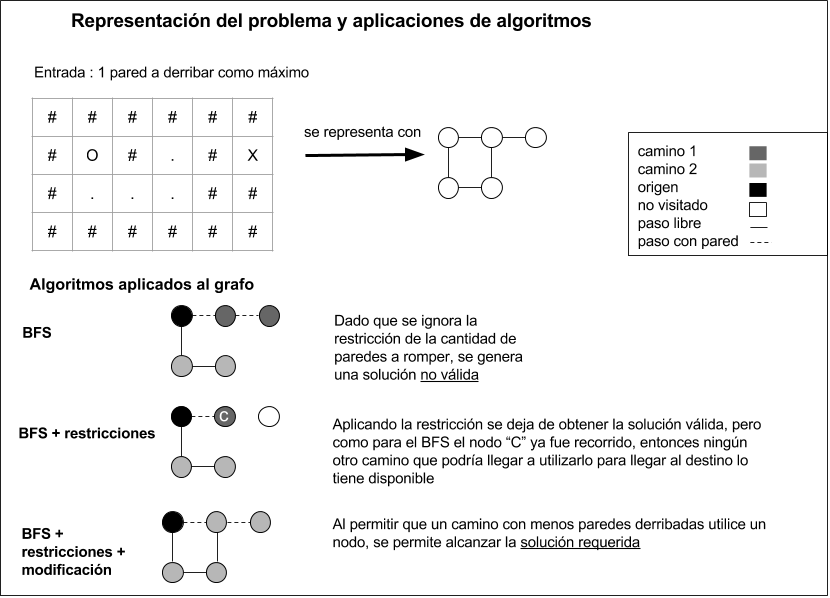
\includegraphics[scale=0.6]{./EJ1/ej1-explicacion.png}
  \end{center}
  \vspace*{0.3cm}

Para poder calcular todos los caminos que pueden llegar efectivamente al destino, en cada nodo se guardará las caracteristicas de tiempo y paredes necesarias para alcanzarlo:
\begin{itemize}
\item Si no ha sido alcanzado, entonces, se guarda el estado en el que se encuentra el nodo desde donde hacemos la visita: si se atravezo una o más paredes para lograrlo, se marca en su estado, al igual que el tiempo insumido en alcanzarlo.
\item Si ya ha sido alcanzado, entonces si la cantidad de paredes rotas hasta llegar hasta él por el camino actual es menor a la cantidad de paredes que fueron rotas anteriormente, entonce se considera que el camino actual es la mejor forma de alcanzar al nuevo nodo, guardando los datos del camino actual en el nodo.
\item En el caso de que alcanzar al nodo previamente visitado, demande el mismo tiempo y esfuerzo que en el camino actual, se desestima el camino actual.
\item Si el nodo a evaluar es el destino, se da por finalizado el algoritmo y se devuelve el estado del camino que lo alcanzó.
\end{itemize}
\subsection{Pseudoc\'odigo}
\begin{algorithm}[H] %or another one check
 \caption{Algoritmo EJ1}
 %     \SetAlgoLined
	encolo nodo origen en una cola de nodos \\
	    \While{$\neg$ cola vacia)}{
	    Nodo actual $\gets$ tope cola \\
	    procesar vecinos\\
	    }
	    
\end{algorithm}


\begin{algorithm}[H] %or another one check
 \caption{procesarNodo(Nodo nod)}
 	Nodo nod es un vecino de actual en el Mapa\\
	
       	   	 \If{$\#$ paredes rotas hasta actual + esPared(nod) < $\#$ paredes rotas hasta actual nod}{
       	   	 para distancia hasta nod $\gets$ distancia hasta actual + 1\\
       	   	 para $\#$ paredes rotas hasta nod $\gets$ $\#$ paredes rotas hasta actual + esPared(nod) 
			\If{nod = nodo destino}	{
				devolver distancia hasta nodo destino y terminar
			}
	   	   	 \If{$\#$ paredes rotas hasta nod $\leq$ Pmax}{
       	   		 encolar nod 
       	   		 }
       	   } 
			
			
\end{algorithm}


\textbf{Aclaraciones de variables y transformaci\'on de entrada}

\begin{itemize}
\item {\bf Variable Mapa}: la matriz $(N \ast M)$ de nodos.
\item {\bf Tipo Nodo}: Dicho tipo, fue creado para contener m\'as informaci\'on de cada nodo, el mismo esta compuesto por posici\'on i, j del nodo en el Mapa, si es pared o no y por \'ultimo la cantidad de paredes destruidas y la distancia recorrida hasta dicho nodo.
\item {\bf cola}: Como la palabra lo indica, en esta cola se ir\'an encolando los nodos.
\end{itemize}  




\subsection{An\'alisis de complejidades}
\vspace*{1em}

Realizando pasos 2-1, cada solución construída tendrá {\bf a lo sumo n-1 pasos}, siendo n la cantidad total de personas en la comitiva.

En el primer paso se analizan $\binom {n}{2}$ parejas posibles a enviar y por cada una de ellas se eligirá de entre 2 personas para ser el farlero.\\

En el segundo paso se tendran $\binom {n-1}{2}$ parejas posibles y 3 faroleros para elegir.\\

Para el (i)-esimo paso se tendrán $\binom {n-(i-1)}{2}$ parejas e i+1 faroleros.\\

Por cada una de las posibilidades de cada paso, se deberan analizar la cantidad total de
posibilidades que haya en el paso subsiguiente, para dar lugar asi al analisis de todas las combinaciones posibles, es decir: siendo que el segundo paso se ejecuta $2 \ast \binom {n}{2}$ veces, el tercero $2 \ast \binom {n}{2} \binom{n-1} {2} \ast 3$, podemos ver que en combinación, todos los pasos demandarían:
\[
\prod_{i=1}^{n-1}\binom {n-(i-1)}{2}*(i+1) = \prod_{i=1}^{n-1}\binom {n-(i-1)}{2} * \prod_{i=0}^{n-1}(i+1)
\]

\[
n!\prod_{i=0}^{n-2}\binom {n-i}{2} = n!\prod_{i=0}^{n-2}\frac{(n-i)(n-(i-1))}{2}
\]

\[
\frac{ n!}{2^{n-2}}.\prod_{i=0}^{n-2}(n-i).\prod_{i=0}^{n-2}(n-(i-1)) = \frac{n!}{2^{n-2}}.n!.\frac{(n+1)!}{2}\leq \frac{n!^{2}.(n+1)!}{2^{n-1}}\in O(n.n!^{3})
\]
\subsection{Experimientos y conclusiones}
\subsubsection[1.5]{Testeo y performance del algoritmo}
\indent Para verificar el correcto funcionamiento de nuestro algoritmo , elaboramos disversos tests,
los cuales ser\'an enunciados a continuaci\'on.\\

\begin{center}
 \textbf{Todos los arqueologos y canibales presentan la misma velocidad}
\end{center}

Este caso se da cuando V${\_i}$ = W${\_j}$ $\forall$ (i,j)  $\gets$ [0..6] \\

 Para este tipo de testeo mostraremos a continuaci\'on un ejemplo del mismo, exponiendo su respectivo resultado. Adem\'as veremos mas adelante, que por el desarrollo de nuestro algoritmo y sus respectivas podas este ser\'a el peor caso en referencia a la perfomance del mismo.\\
 
 Con un:
\begin{flushleft}
	$Cantidad$ $de$ $arqueologos:$ $4 $  \\
	$Cantidad$ $de$ $canibales:$ $2 $  \\
	$Velocidad$ $de$ $arqueologos:$ $10$ $10$ $10$ $10$  \\
	$Velocidad$ $de$ $canibales:$ $10$ $10 $  \\
 \end{flushleft}	
  Obtuvimos el siguiente resultado:
\begin{flushleft}  
  $Velocidad$ $de$ $cruce$ $total: $\\
 \end{flushleft}


 \begin{center}
 \textbf{No hay canibales}
\end{center}

Esta versi\'on se da cuando M = 0. 

Para este tipo de testeo mostraremos a continuaci\'on un ejemplo del mismo, exponiendo su respectivo resultado.\\

 Con un:
 \begin{flushleft}
  	$Cantidad$ $de$ $arqueologos:$ $5 $  \\
	$Cantidad$ $de$ $canibales:$ $0 $  \\
	$Velocidad$ $de$ $arqueologos:$ $15$ $10$ $5$ $2$ $20$  \\
	$Velocidad$ $de$ $canibales: $  \\
\end{flushleft}
  Obtuvimos el siguiente resultado:
  \begin{flushleft}
$Velocidad$ $de$ $cruce$ $total: $\\
\end{flushleft}
\begin{center}
 \textbf{Todos los arqueologos y canibales presentan velocidades distintas}
\end{center}

Este caso se da cuando V${\_i}$ $\neq$ W${\_j}$ $\forall$ (i,j)  $\gets$ [0..6] 

Aqu\'i veremos, un ejemplo del conjunto de test de este tipo, exponiendo su respectivo resultado.\\

 Con un:
 \begin{flushleft} 
  	$Cantidad$ $de$ $arqueologos: 3 $  \\
	$Cantidad$ $de$ $canibales: 3 $  \\
	$Velocidad$ $de$ $arqueologos:$ $2$ $4$ $6 $  \\
	$Velocidad$ $de$ $canibales:$ $1$ $3$ $5 $  \\
\end{flushleft}
  Obtuvimos el siguiente resultado:
   \begin{flushleft}   
$Velocidad$ $de$ $cruce$ $total: $\\
\end{flushleft}

\begin{center}
 \textbf{Hay un canibal cada dos arqueologos}
\end{center}

Este tipo de caso se cumple cuando N = 2 $\ast$ M

Un ejemplo que simboliza el conjunto de test de este tipo es el siguiente:\\

 Con un:
 \begin{flushleft} 
  	$Cantidad$ $de$ $arqueologos:$ $4 $  \\
	$Cantidad$ $de$ $canibales:$ $2$ \\ 
	$Velocidad$ $de$ $arqueologos:$ $3$ $6$ $9$ $12$\\
	$Velocidad$ $de$ $canibales:$ $1$ $2$  \\
\end{flushleft}
  Obtuvimos el siguiente resultado:
   \begin{flushleft}   
$Velocidad$ $de$ $cruce$ $total: $\\
\end{flushleft}


\begin{center}
 \textbf{Hay mas canibales que arqueologos}
\end{center}

Este tipo de caso se cumple cuando N < M

A continuaci\'on enunciaremos, un ejemplo del conjunto de test de este tipo, exponiendo su respectivo resultado.\\

 Con un:
 \begin{flushleft} 
  	$Cantidad$ $de$ $arqueologos:$ $2 $  \\
	$Cantidad$ $de$ $canibales:$ $3$ \\ 
	$Velocidad$ $de$ $arqueologos:$ $3$ $6$ \\
	$Velocidad$ $de$ $canibales:$ $1$ $2$ $5$  \\
\end{flushleft}
  Obtuvimos el siguiente resultado:
   \begin{flushleft}   
$Velocidad$ $de$ $cruce$ $total:$ \textit{NO HAY SOLUCI\'ON} \\
\end{flushleft}




\newpage
\section{Ejercicio 2} 
\subsection{Explicaci\'on de resoluci\'on del problema}
En esta ocasión se debe encontrar, dada una serie de habitaciones, la forma menos costosa de unirlas, teniendo que derribar determinadas paredes para lograrlo. Dada 2 habitaciones: el muro menos costoso para derribar que las une será la elección a tomar para formar la solución, es decir, se deben elegir todos los muros menos costosos que unen las distintas habitaciones para obtener la solucion buscada.

Un planteo de modelo sobre grafo caracteriza a cada habitación como un conjunto de puntos caminables y cada uno de estos como un nodo adyacente a los puntos de la misma habitacion, el cual posee H componentes conexas, siendo H la cantidad total de habitaciones en el mapa. Lo que se busca entonces es una forma de unir estas componentes de la forma menos costosa. Para ello las unimos a 2 habitaciones separadas por una pared con un eje de peso igual al esfuerzo de derribarla. A las aristas de las componentes les asignamos el peso nulo.

CLAVAR EL DRAWING

Para obtener la solucion, se busca el AGM del grafo planteado mediante el algoritmo de Kruskal; a él se le calcula el peso, el cual representa la respuesta al problema.


\subsection{Pseudoc\'odigo}
\begin{algorithm}[H] %or another one check
\Fn{Balancear()}{
	entero sumaParcial $\gets$ 0 \hfill O(1)\\ 
	arreglo sumasParciales \hfill O(1)\\ 
    \While{sumaParcial $\leq$ P}{ 
    \hfill ciclo: O(log(P))\\
      sumasParciales $\cup$ sumaParcial \hfill O(1)\\
	para sumaParcial asignar sumaParcial + 3$^{i}$ \hfill O(1)\\
     	incrementar i \hfill O(1)\\
     }
	entero indice $\gets$ size(sumasParciales)-1  \hfill O(1) \\
	entero equilibrioActual $\gets$ P \hfill O(1)\\
	entero potenciaActual $\gets$ 0 \hfill O(1)\\ 
	    \While{|equilibrioActual| $>$ 0}{
	    		\hfill ciclo: O(log(P))\\ 
	          \If{sumasParciales[indice-1] $<$ |equilibrioActual| $\leq$ sumasParciales[indice]}{
	          	\hfill guarda: O(1)\\ 
	          
       para potenciaActual asignar sumasParciales[indice] -  sumasParciales[indice-1] \hfill O(1)\\ 
       
       	\eIf{equilibrioActual $<$ 0}{ 
       	   	para equilibrioActual asignar potenciaActual + equilibrioActual \\
                platoDerecho $\cup$ potenciaActual \hfill O(1)\\ 
		}{
			para equilibrioActual asignar equilibrioActual - potenciaActual \\
                platoIzquierdo $\cup$ potenciaActual \hfill O(1)\\ 
      	}
     }
     indice--	\hfill O(1)\\ 
	}
	devolver size(platoDerecho) \hfill O(1)\\   
		devolver size(platoIzquierdo) \hfill O(1)\\     
			devolver invertir(platoDerecho) \hfill O(1)\\      
				devolver invertir(platoIzquierdo) \hfill O(1)\\ 
   } 

\textbf{\hfill total: O(log(P))}\\ 
\end{algorithm}

\subsection{An\'alisis de complejidades}

Nuestro algoritmo como mencionamos anteriormente presenta 3 etapas.\\
La primera de ellas consta en recorrer desde $3^0$ hasta $3^i$ donde este ultimo sea igual a $P$ o en su defecto el inmediato mayor. Por lo tanto mostraremos que recorrer hasta un i donde $3^i$ sea igual o inmediatamente mayor a P es menor o igual a $\sqrt{P}$.\\


Si $i = 0$ $\Rightarrow$ terminamos.\\
Luego sea $3^i \geq P \geq 3^{i-1}$ con $i > 0$. Queremos ver que $i \leq \sqrt{P}$:\\
Se que por definici\'on $P \geq 3^{i-1}$ $\Rightarrow$ $\sqrt{P} \geq \sqrt{3^{i-1}}$\\
Veamos que $\sqrt{3^{i-1}} \geq i \Rightarrow 3^{i-1} \geq {i^2}$. Para $i = 1$ tenemos que $3^{1-1} \geq 1$ siempre. Luego, para $i > 1$ como ${3^{i-1}}$ es creciente y mayor o igual que $i^2$ se cumple siempre esta desigualdad. Por lo tanto queda probado que recorrer hasta un i tal que $3^i \geq P$ se encuentra en el orden de  O($\sqrt{P}$).\\


 Luego, creamos dos enteros \textit{saldoEnBalanza} y \textit{N} y un array \textit{arrayPesasUtilizadas} inicializado vacio, por lo tanto, como son enteros y el array es vacio esto insume O(1), finalizando as\'i la primera etapa.\\
Luego, la segunda etapa y m\'as importante de nuestro algoritmo, consiste en un ciclo donde realizaremos iterativamente la busqueda de las pesas que, sumando sus valores, nos de el valor $P$. Dicho ciclo en el peor de los casos recorrer\'a desde el valor de i que conten\'ia la pesa de mayor valor hasta i = 0, lo cual ser\'a O($\sqrt{P}$) ya que al trabajar con potencias de 3 la cantidad de vueltas del ciclo entraran en el orden de $\sqrt{P}$ como hab\'iamos demostrado anteriormente.\\ 

Dentro de este ciclo, realizamos 6 comparaciones en O(1) las cuales son:

\begin{itemize}
\item si N=0, si N=1, aqu\'i agregamos el valor de la pesa al array y terminamos el ciclo, esto insumir\'a O(1)
 \item si N es menor al valor de \textit{saldoEnBalanza}, estas opcion no finaliza el ciclo,
 agrega la pesa n el array, modifica el valor de saldoEnBalanza por el valor de N y disminuye en 1 a i, luego se chequea aqui mismo si $N < 0$ de ser verdadero se modifica el valor de $estaEnNegativo$ por verdadero o por falso en caso de ser falsa la guarda, lo cual insumir\'a O(1) cada una de las operaciones mencionadas, luego se chequea aqui mismo si $N < 0$ de ser verdadero se modifica el valor de $estaEnNegativo$ por verdadero o por falso en caso de ser falsa la guarda
 \item por ultimo, si $N \geq saldoEnBalanza$ solamente descontamos en uno a i para continuar con el ciclo.
\end{itemize} 
Una vez finalizado esto y por consiguiente la segunda etapa, pasamos a la tercera la cual consiste en guardar en \textit{arrayI} o \textit{arrayD} los valores de los elementos del \textit{arrayPesasUtilizadas} para colocarlos en la balanza del lado derecho o del izquierdo.\\
Para realizar esto recorremos el array \textit{arrayPesasUtilizadas} el cual en el peor de los casos tendr\'a todas las pesas, lo cual como vimoss recorrer la totalidad de elementos del array se encuentra en el orden de O($\sqrt{P}$).\\

Luego de ver esto, dentro del ciclo realizamos operaciones en O(1).\\
Por ultimo, devolvemos los array invirtiendo las posiciones de los elementos lo que insumir\'a en el peor de los caso O($\sqrt{P}$).\\

En conclusi\'on nuestro algoritmo realiza 4 ciclos que demandan en el peor de los casos O($\sqrt{P}$) donde dentro de los mismos se realizan operaciones en O(1), por lo tanto nuestra complejidad final ser\'a
O($\sqrt{P}$).





\subsection{Experimientos y conclusiones}
Nuestro algoritmo chequea en cada paso si existe alg\'un gimnasio capaz de ser vencido y, si existe, busca cual es el m\'as cercano, por lo tanto existir\'an casos en los cuales la soluci\'on obtenida para los mismos sea la \'optima pero para algunos no lo ser\'a.

\subsubsection*{Familias con soluci\'on obtenida igual a la \'optima}

%\begin{enumerate}
%\item No se obtiene soluci\'on por no haber las pokeparadas necesarias para ganar en todos los gimnasios.
%\item No se obtiene soluci\'on ya que la capacidad de la mochila no puede contener las pociones necesarias para vencer a un cierto gimnasio.
%\item Todos los gimnasios sin necesidad de pociones para ser vencidos.
%\item Las pokeparadas y los gimnasios se reciben en orden de la forma en la cual exista una pokeparada puntual para ir a cada gimnasio
%\end{enumerate}

\begin{center}
\textbf{Familia 1 y 2}
\end{center}

Ambas familias devolverán -1 ya que como se explicó anteriomente tanto el greedy como el exacto presentan podas para estos casos sin soluci\'on por lo tanto, su tiempo de ejecuci\'on ser\'a aproximadamente el mismo. \\\\

\begin{figure}[h]
 \centering
  \subfloat[Familia 1: actua poda 1]{
    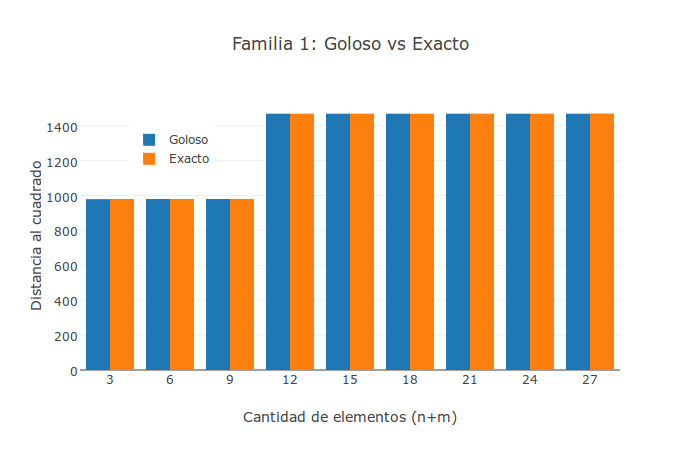
\includegraphics[width=0.45\textwidth]{./EJ2/fam1medicion.png}}
       \label{fig:fam1medicion}
  \subfloat[Familia 2: actua poda 2]{
    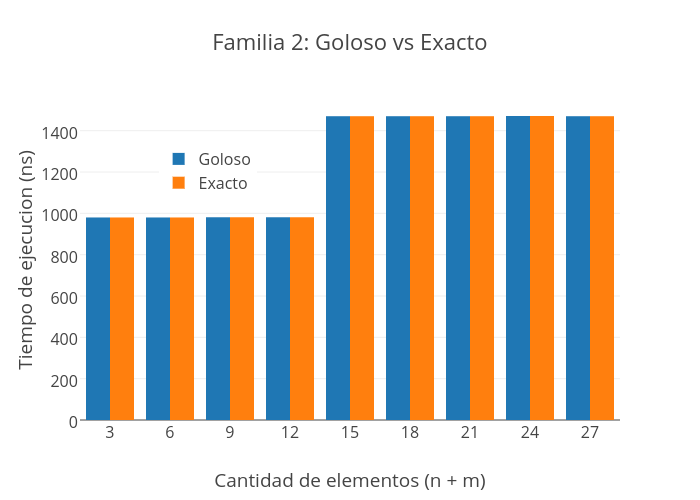
\includegraphics[width=0.45\textwidth]{./EJ2/fam2medicion.png}}
    \label{fig:fam2medicion}
    \end{figure}

Como se observa en los \'ultimos gr\'aficos, las funciones resultantes para cada familia en ambos algoritmos presentan el mismo tiempo por lo comentando sobre las podas realizadas.

\begin{center}
\textbf{Familia 3}
\end{center}

En este caso, como nuestro greedy chequea si hay alg\'un gimnasio a ser vencido con la cantidad de pociones que se tienen en el momento (se inicia con 0), y como todos necesitan 0, recorre los gimnasios sin necesidad de pasar por las pokeparadas, obteniendo la mejor soluci\'on posible.

A continuaci\'on mostraremos el camino obtenido tanto para el algoritmo exacto como el goloso de un caso en el que se trabaja con 8 elementos en total para ejemplificar lo enunciado anteriormente:

   \vspace*{0.3cm} \vspace*{0.3cm}
  \begin{center}
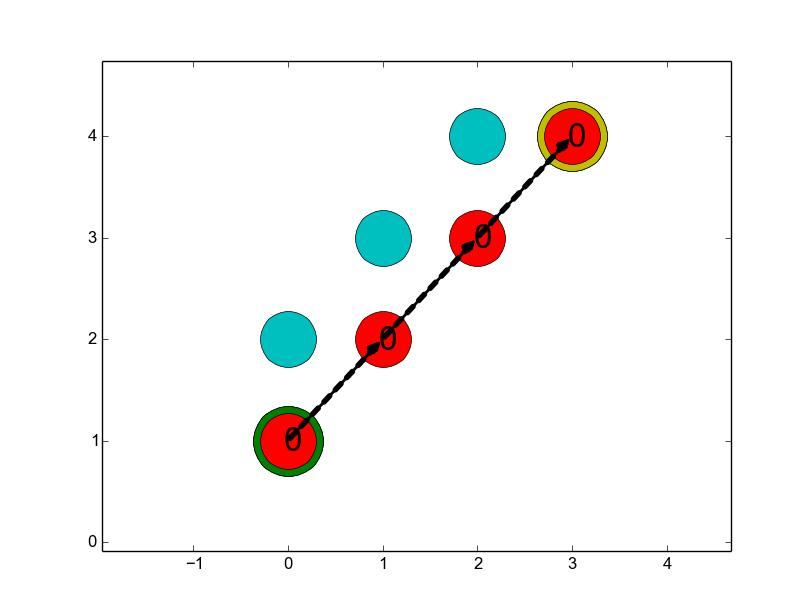
\includegraphics[scale=0.40]{./EJ2/todos0.png}
\\{\textit{Punteado = resultado exacto, contínua = resultado goloso}}
  \end{center}
  \vspace*{0.3cm}

Como se observa en el ejemplo el camino obtenido es exactamente el mismo.

\begin{center}
\textbf{Familia 5}
\end{center}

Se obtendr\'a la soluci\'on \'optima para esta familia ya que se reciben primero pokeparadas para vencer a un gimnasio cerca del mismo y luego m\'as pokeparadas para vencer a otros gimnasios que se encuentren cerca de los mismos. Se mostrar\'a a continuaci\'on un dibujo que ejemplifica lo dicho:

\vspace*{0.3cm} \vspace*{0.3cm}
  \begin{center}
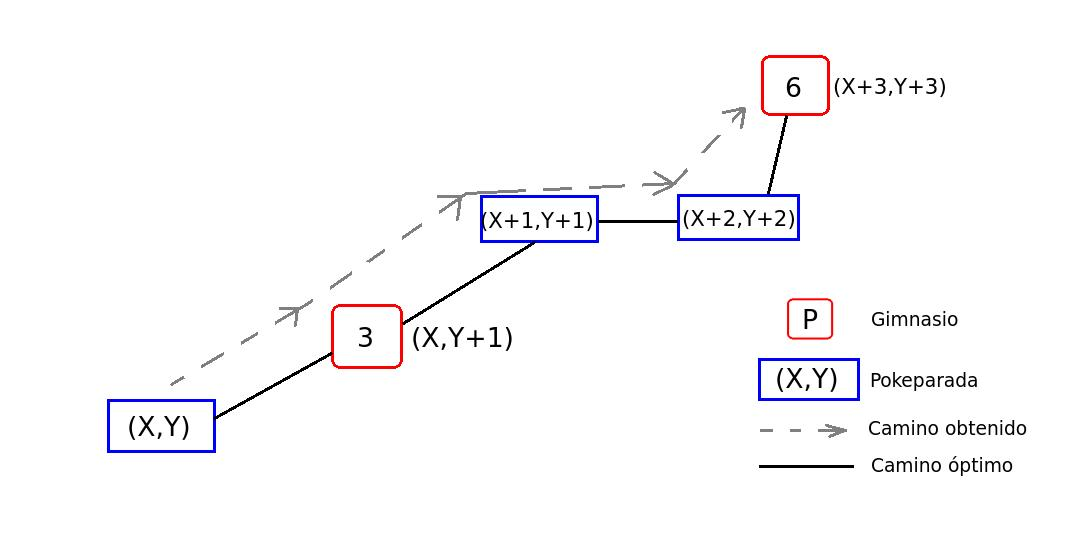
\includegraphics[scale=0.30]{./EJ2/optima.jpeg}
\\{\textit{Punteado = resultado exacto, contínua = resultado goloso}}
  \end{center}
  \vspace*{0.3cm}

\subsubsection*{Familia con soluci\'on no \'optima}

\begin{center}
\textbf{Familia 4}
\end{center}

En este tipo de familia existan gimnasios que no necesiten pociones para ser vencidos y otros que si. Nuestro algoritmo, por cada iteraci\'on chequea si puede elegir un gimnasio que se encuentre a una distancia m\'inima en relaci\'on a los demás, y adem\'as corrobora si posee las pociones necesarias para vencerlo, decide inicialmente ir a vencer a los gimnasios que posean cero poder, lo cual puede no ser \'optimo para el resultado final.

Este es un ejemplo del algoritmo exacto y el goloso con un total de 10 elementos:

\begin{figure} [!ht]
 \centering
  \subfloat[Algoritmo exacto]{
    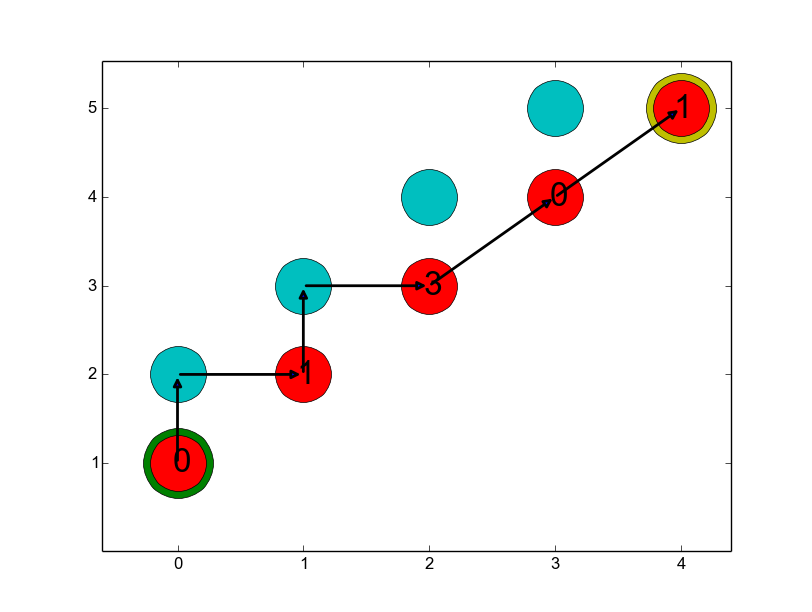
\includegraphics[width=0.45\textwidth]{./EJ2/fam5exacto.png}}
       \label{fig:fam5exacto}
  \subfloat[Algoritmo goloso]{
    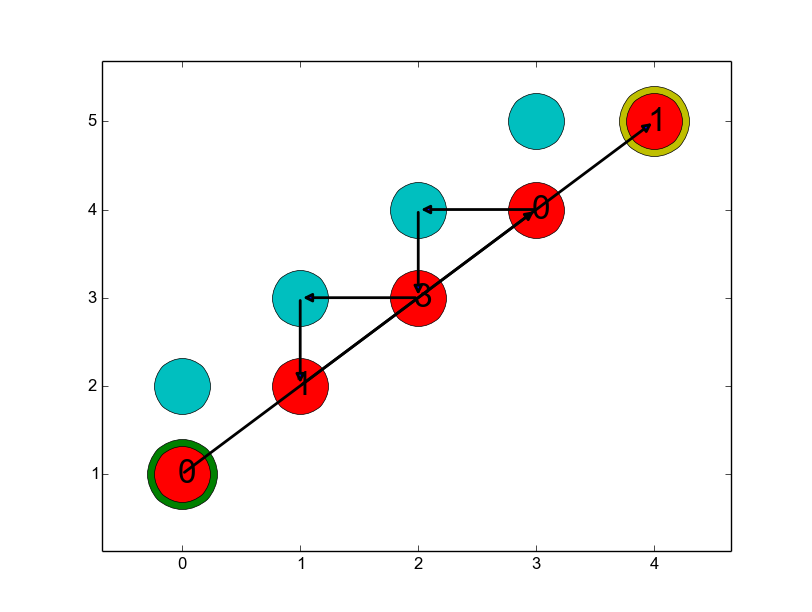
\includegraphics[width=0.45\textwidth]{./EJ2/fam5goloso.png}}
    \label{fig:fam5goloso}
    \end{figure}
    
Con respecto a la diferencia entre la soluciones que se obtienen en relacion a las óptimas elebaramos las siguientes comparaciones:\\\\
 

  \begin{figure} [h]
 \centering
  \subfloat[Comparación de distancias obtenidas]{
    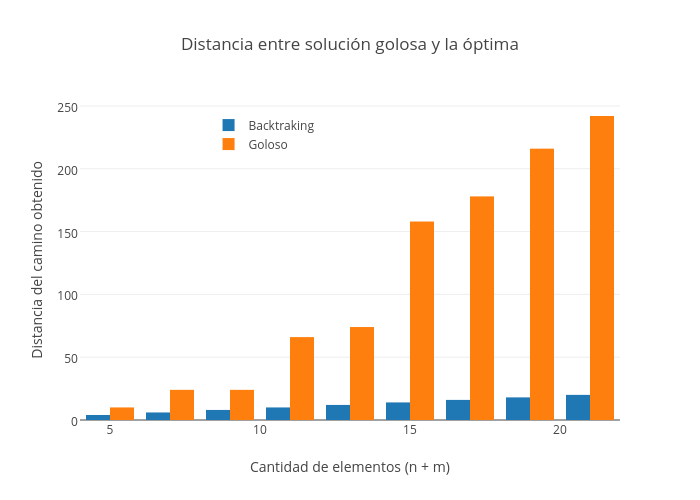
\includegraphics[width=0.5\textwidth]{./EJ2/gym0Dif.png}
    \label{fig:comparativo31}}
  \subfloat[Porcentaje de error relativo del goloso]{
    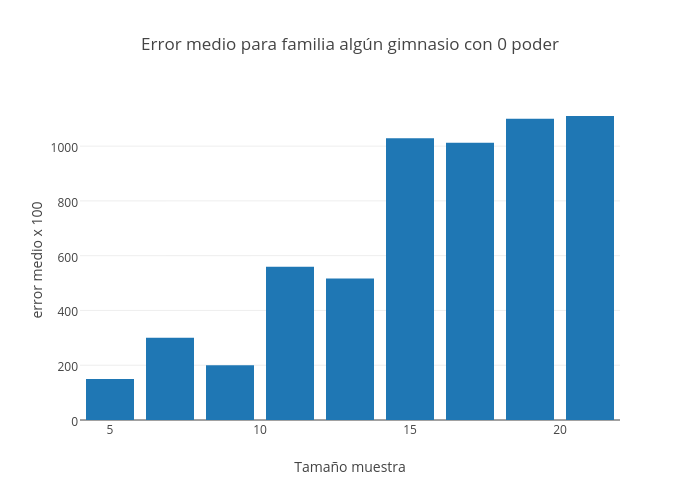
\includegraphics[width=0.5\textwidth]{./EJ2/gym0Error.png}
    \label{fig:comparativo32}}
    \end{figure} 
 
Debido al poder de cómputo utilizado para realizar los tests, solo pudo testearse el algoritmo exacto hasta con 20 elementos teniendo que bajar inclusive hasta 15 elementos para algunas familias, mientras que el goloso puede tomar una mayor cantidad de elementos con tiempos de ejecución considerablemente menores.

\begin{center}
\textbf{Familia 6}
\end{center}

Este estilo de familia presenta a los gimnasios y pokeparadas desordenados en referencia a las posiciones, es decir, para ganar a cierto gimnasio es necesario pasar por una cantidad puntual de pokeparadas las cuales estan de un lado y del otro de dicho gimnasio.
\\\\

  \begin{figure} [h]
 \centering
  \subfloat[Comparación de distancias obtenidas]{
    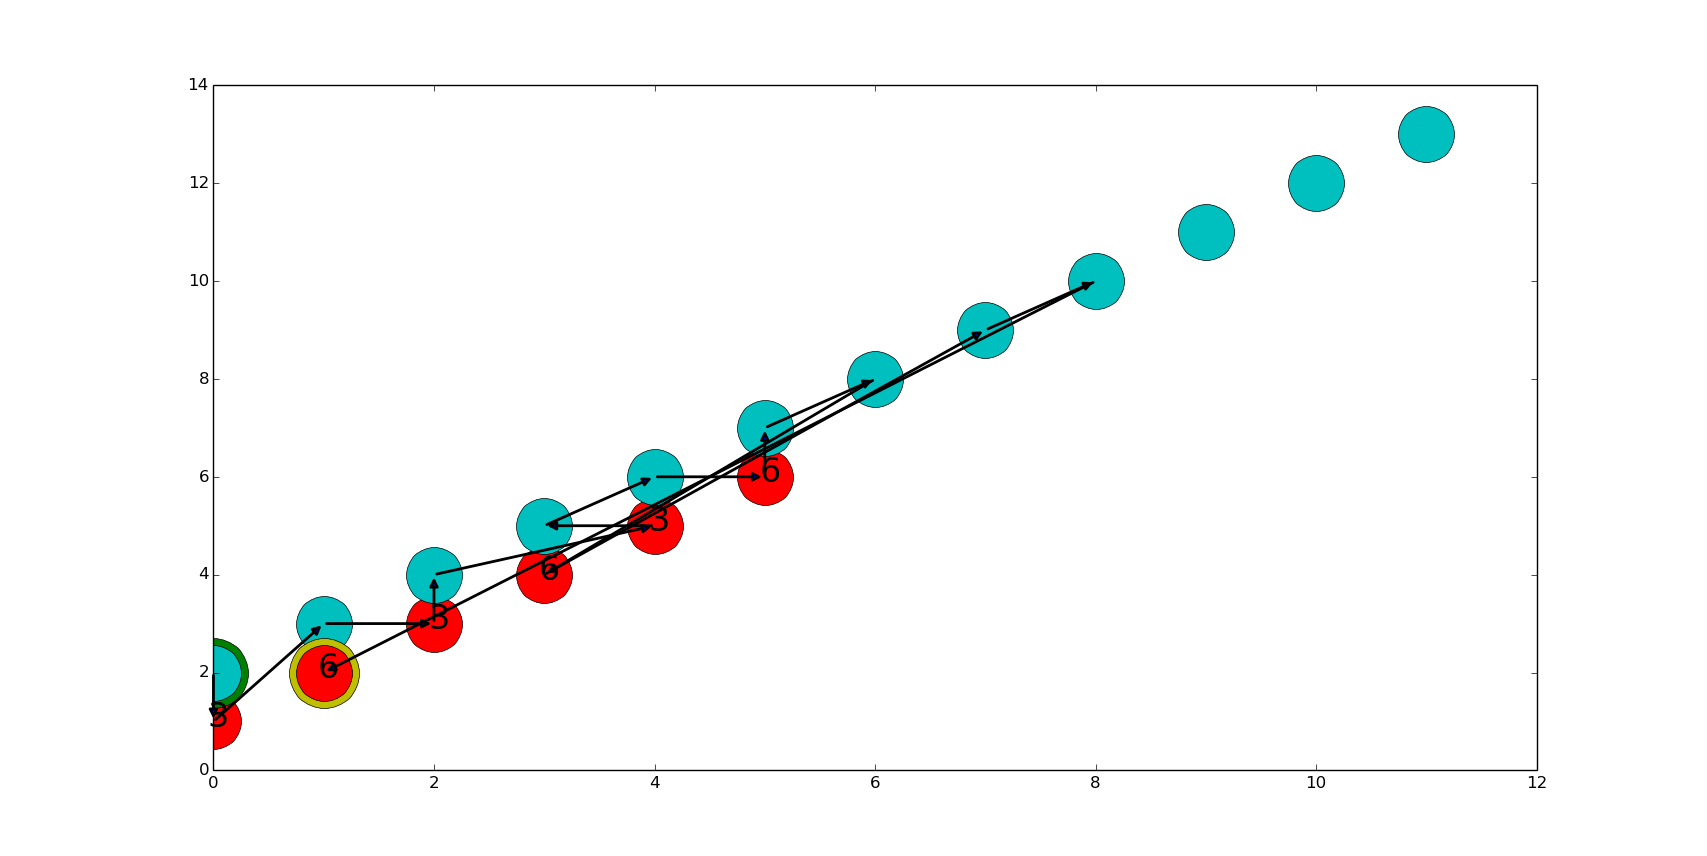
\includegraphics[width=0.50\textwidth]{./EJ2/caminosinorden1.png}
    \label{fig:caminosinorden1}}
  \subfloat[Porcentaje de error relativo del goloso]{
    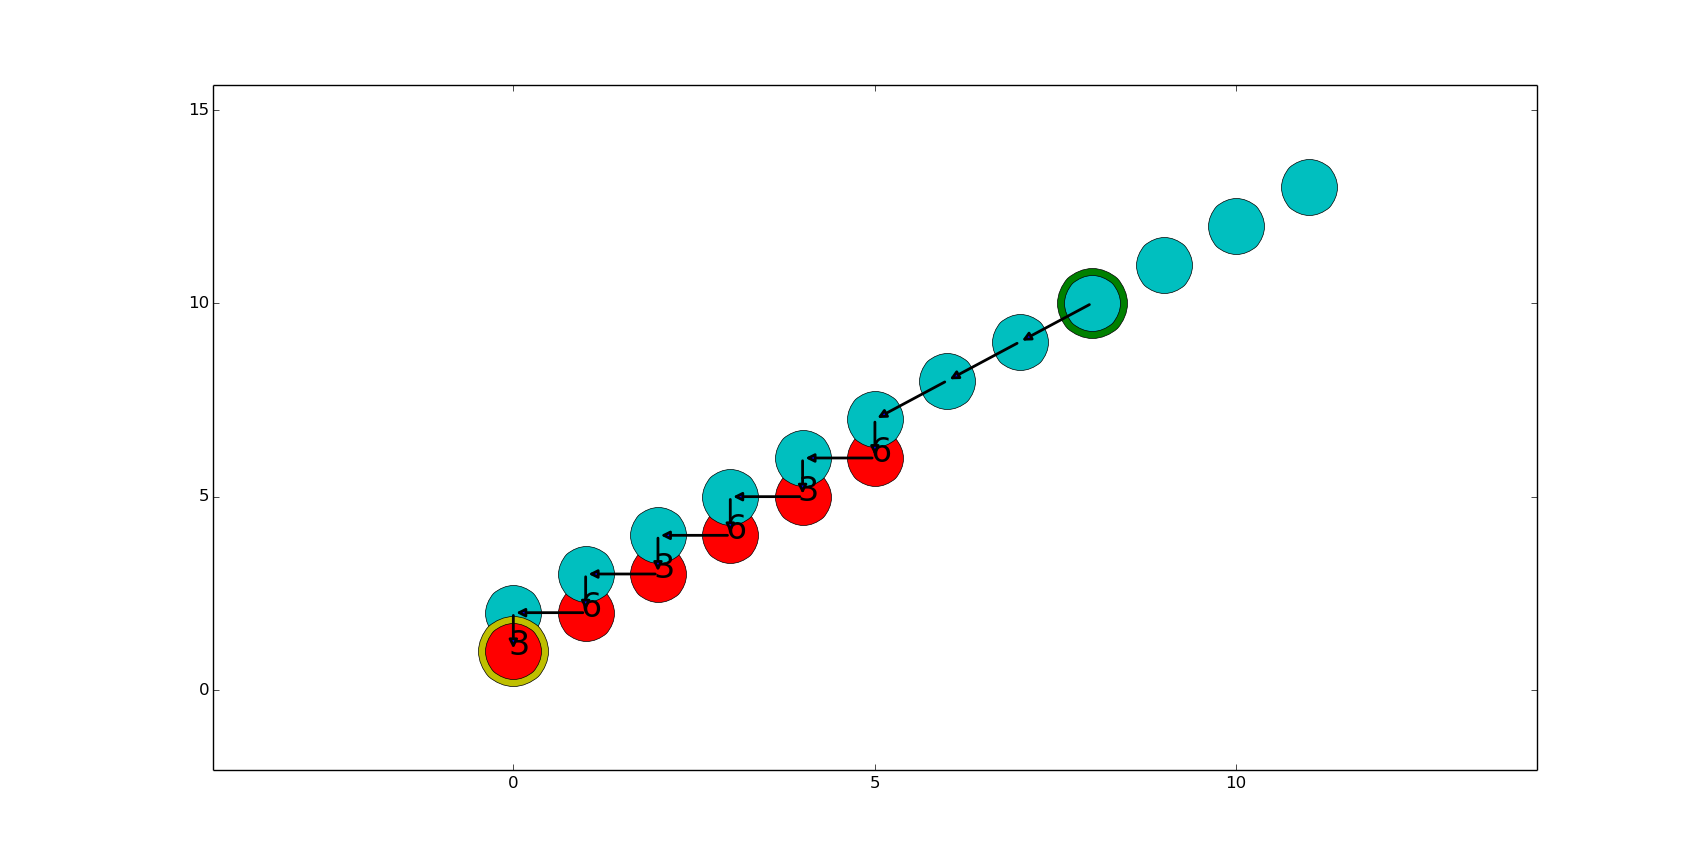
\includegraphics[width=0.50\textwidth]{./EJ2/caminosinorden.png}
    \label{fig:caminosinorden}}
    \end{figure} 

Se puede observar en el ejemplo como nuestro algoritmo goloso va a la primer pokeparada y de ah\'i a vencer al gimnasio m\'as cercano en vez de ir a la pokeparada consecutiva. Esto lo hace hasta vencer a todos los gimnasios.

La diferencia entre soluciones se pueden apreciear en los siguientes gràficos:\\

  \begin{figure} [h]
 \centering
  \subfloat[Comparación de distancias obtenidas]{
    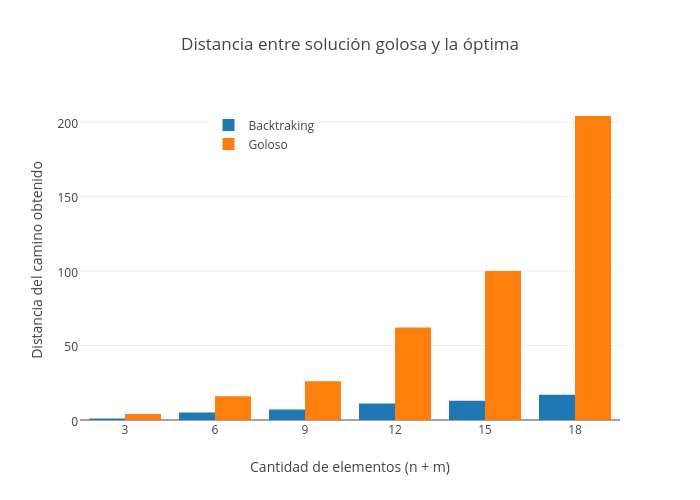
\includegraphics[width=0.50\textwidth]{./EJ2/sinOrdenDif.png}
    \label{fig:comparativo31}}
  \subfloat[Porcentaje de error relativo del goloso]{
    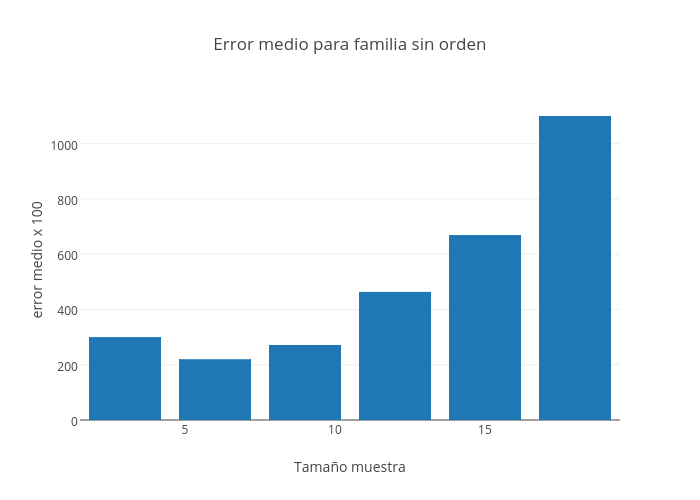
\includegraphics[width=0.50\textwidth]{./EJ2/sinordenError.png}
    \label{fig:comparativo32}}
    \end{figure} 

\begin{center}
\textbf{Familia 7}
\end{center}

El objetivo de esta familia es plantear un caso en donde, de forma controlada, la respuesta del algoritmo goloso nunca fuera la óptima. Para ello, se genera una instancia agrupando los gimnasios y pokeparadas en 2 anillos de radios diferentes. Dado que nuestro algoritmo siempre y cuando pueda vencer a alg\'un gimnasio buscará el m\'inimo en  distancia para vencerlo, para esta familia resultará contraproducente: es preferible adquirir m\'as pociones para luego ir a varios gimnasios juntos, que ganar apenas exista la posibilidad.

\newpage

\vspace*{0.3cm} \vspace*{0.3cm}
\begin{figure} [!ht]
 \centering
  \subfloat[Algoritmo exacto]{
    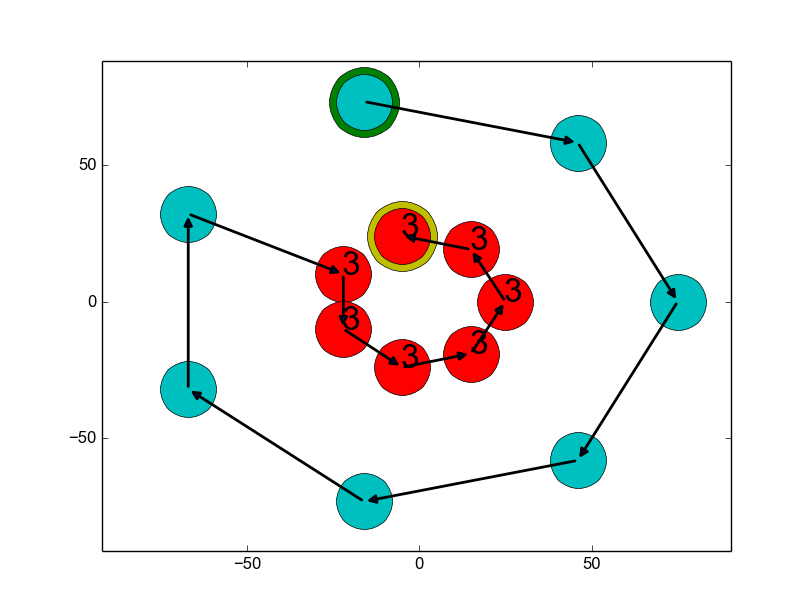
\includegraphics[width=0.45\textwidth]{./EJ2/anilloexacto.png}}
       \label{fig:anilloexacto}
  \subfloat[Algoritmo goloso]{
    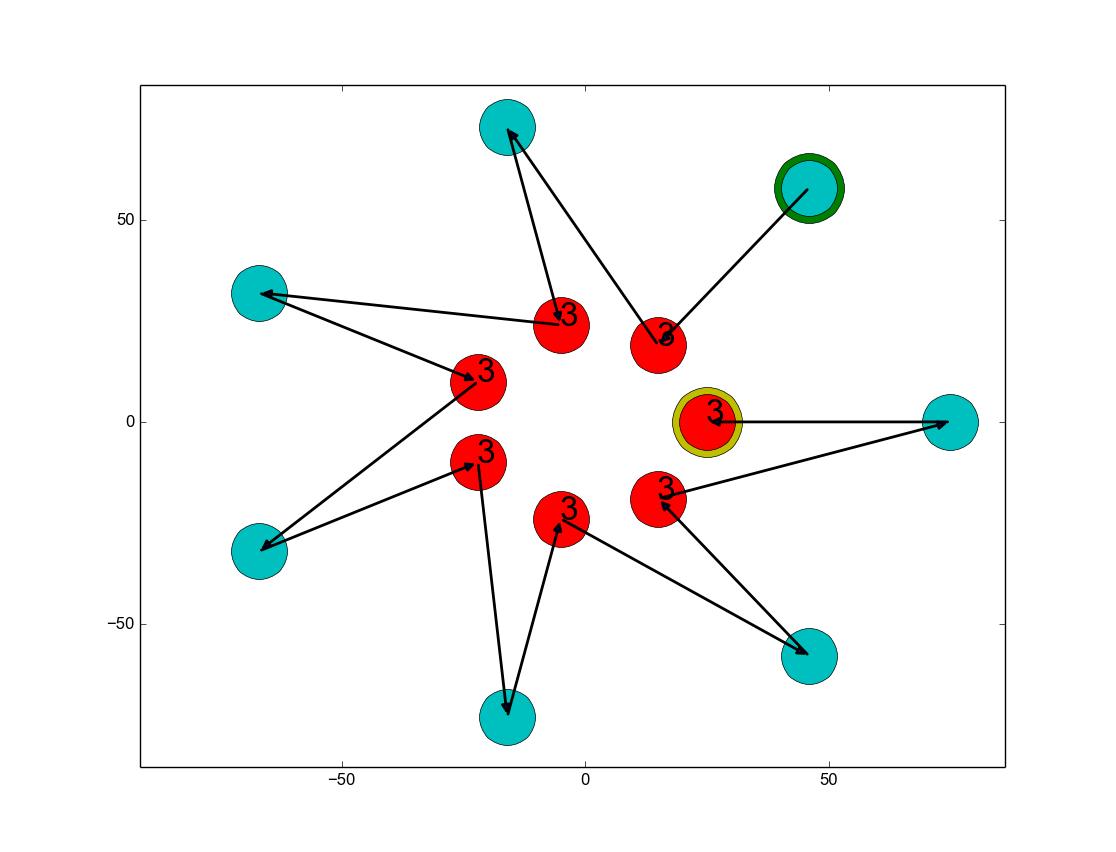
\includegraphics[width=0.45\textwidth]{./EJ2/anillogoloso.png}}
    \label{fig:anillogoloso}
    \end{figure}
\vspace*{0.3cm} \vspace*{0.3cm}

Se puede observar en el \'ultimo gr\'afico como los resultados tienen valores diversos para casos pequeños. En las instancias de mayor tamaño, las solución óptima resulta de recorrer primero todas las pokeparadas y luego los gimnasios, ya que la cantidad de pociones necesarias para vencer a todos los gimnasios es igual a la cantidad total de pociones presentes en el mapa, sumado a que la distancia entre pokeparadas es muy inferior que entre pokeparadas y gimnasios.

Al generarse un camino alternado para el goloso entre gimnasio y pokeparada, se le dan a todos los gimnasios la dificultad igual a la cantidad de pociones que aporta cada pokeparada y se crean la misma cantidad de gimnasios como de pokeparadas. En cuanto a la distribución de los mismos, se buscó una forma de estrella, en la cual cada pokeparada está alineada con 2 gimnasios y una segunda pokeparada. Dadas estas restricciones se observa lo siguiente:

\vspace*{0.3cm} \vspace*{0.3cm}
  \begin{center}
 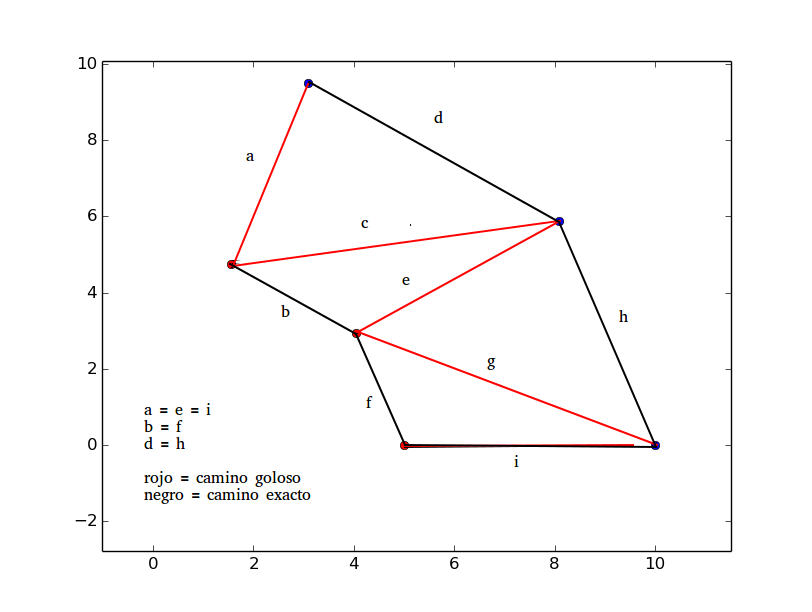
\includegraphics[width=0.75\textwidth]{./EJ2/dibujoorientativo.png}
\\{\textit{Comparación solución golosa vs exacta}}
  \end{center}

El camino goloso realiza un camino de longitud $\sum^{k}_{i=1}a + \sum^{j}_{i=1}c$ y el exacto $\sum^{n-1}_{i=1}b + \sum^{m-1}_{i=1}d + a$. Siendo $k$ el número de aristas como $a$ y $j$ como $c$, se tiene que $k + j = n+m-1$ (aristas en un camino de n+m elementos) y que $k=j+1$. Para que el algoritmo goloso difiera del exacto, se debe cumplir entonces la siguiente desigualdad:
\[
\sum^{k}_{i=1}a + \sum^{j}_{i=1}c \ge \sum^{n-1}_{i=1}b + \sum^{m-1}_{i=1}d + a
\]

La cual equivale a decir:

\[
\sum^{k}_{i=1}a + \sum^{j}_{i=1}c - a \ge (n-1)b + (m-1)d
\]

\[
\sum^{j}_{i=1}a + \sum^{j}_{i=1}c \ge (n-1)b + (m-1)d
\]

\[
j(a + c)\ge (n-1)b + (m-1)d
\]

Siendo que $n=m$ por como se construye la instancia, entonces:


\[
j(a + c) \ge (n-1)(b + d)
\]

Finalmente, como $k = j + 1 \wedge k+j=n+m-1 \leftrightarrow j = n - 1 $, se resolverán distintos caminos siempre y cuando $a +c \ge b + d$. Con lo cual, para generar correctamente las instancias para esta famila, se considero dicha desigualdad.

Podemos ver un ejemplo de la desigualdad de las soluciones presentes en las siguientes instancias corridas con el algoritmo goloso y el backtraking:
 
 
\vspace*{0.3cm} \vspace*{0.3cm}
\begin{figure} [!ht]
 \centering
  \subfloat[Algoritmo exacto]{
 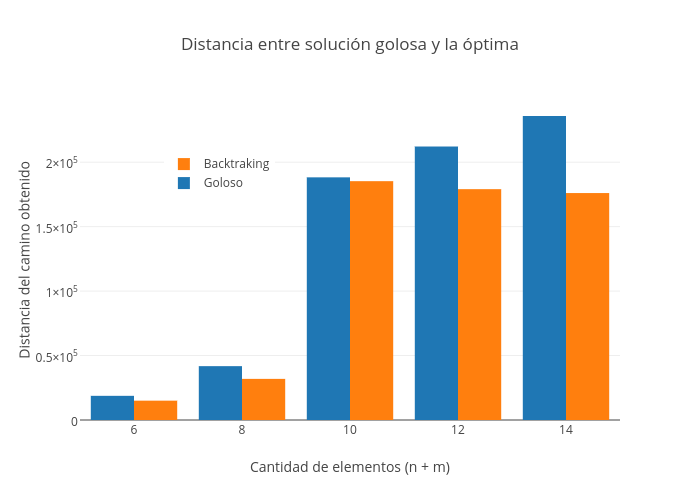
\includegraphics[width=0.5\textwidth]{./EJ2/anillosDif.png}
       \label{fig:anilloexacto}}
  \subfloat[Algoritmo goloso]{
   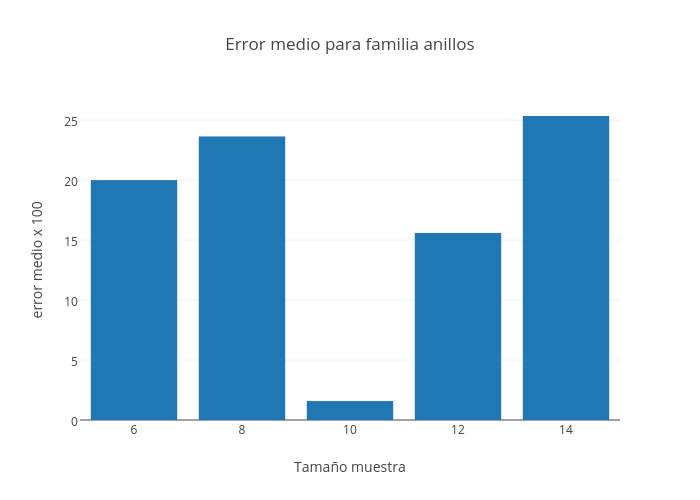
\includegraphics[width=0.5\textwidth]{./EJ2/anillosError.png}
    \label{fig:anillogoloso}}
    \end{figure}

 
Los radios para entradas de hasta 8 elementos son distintos al resto de las instancias. En síntesis se puede ver para los tamaños de 10 a 14 elementos que se mantuvo la distancia recorrida en el algoritmo exacto: esto se debe al carácter del camino, que resulta de recorrer primero una circunferencia, luego dirigirse de forma recta a la circunferencia interior y recorrerla. Al no haber variabilidad en los radios, el tiempo insumido es aproximadamente el mismo. No así para el algoritmo goloso, ya que un incremento en la cantidad de elementos, conyeva un incremento de las idas y vueltas a realizar; aumentando notoriamente la distancia del recorrido.


\subsubsection*{Comparación entre errores de familias}

Teniendo un grupo de familias que provocan soluciones con errores al aplicar el algoritmo goloso, podemos ver lo siguiente entre la Familia 4 y la Familia 6:

\vspace*{0.3cm} \vspace*{0.3cm}
  \begin{center}
 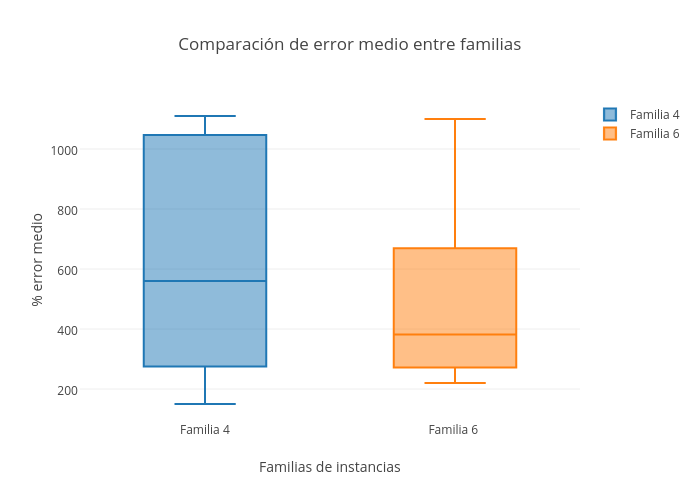
\includegraphics[width=0.75\textwidth]{./EJ2/box.png}
\end{center}

Se evidencia el mejor desempeño del algoritmo sobre la familia 6, provocando un error medio mucho menor que la familia 4 (alrededor de 110\% mejor) y con una dispersión del mismo mucho más baja. 

De forma separada, debido a los rangos que se manejan, se decidió analizar la distribución de la Familia 7. Vale destacar que el error de la misma es muy inferior al de las dos anteriores y posee la menor varianza de todas. Esto se debe al carácter controlado de la misma, y su característica de posicionamiento: 
\vspace*{0.3cm} \vspace*{0.3cm}
  \begin{center}
 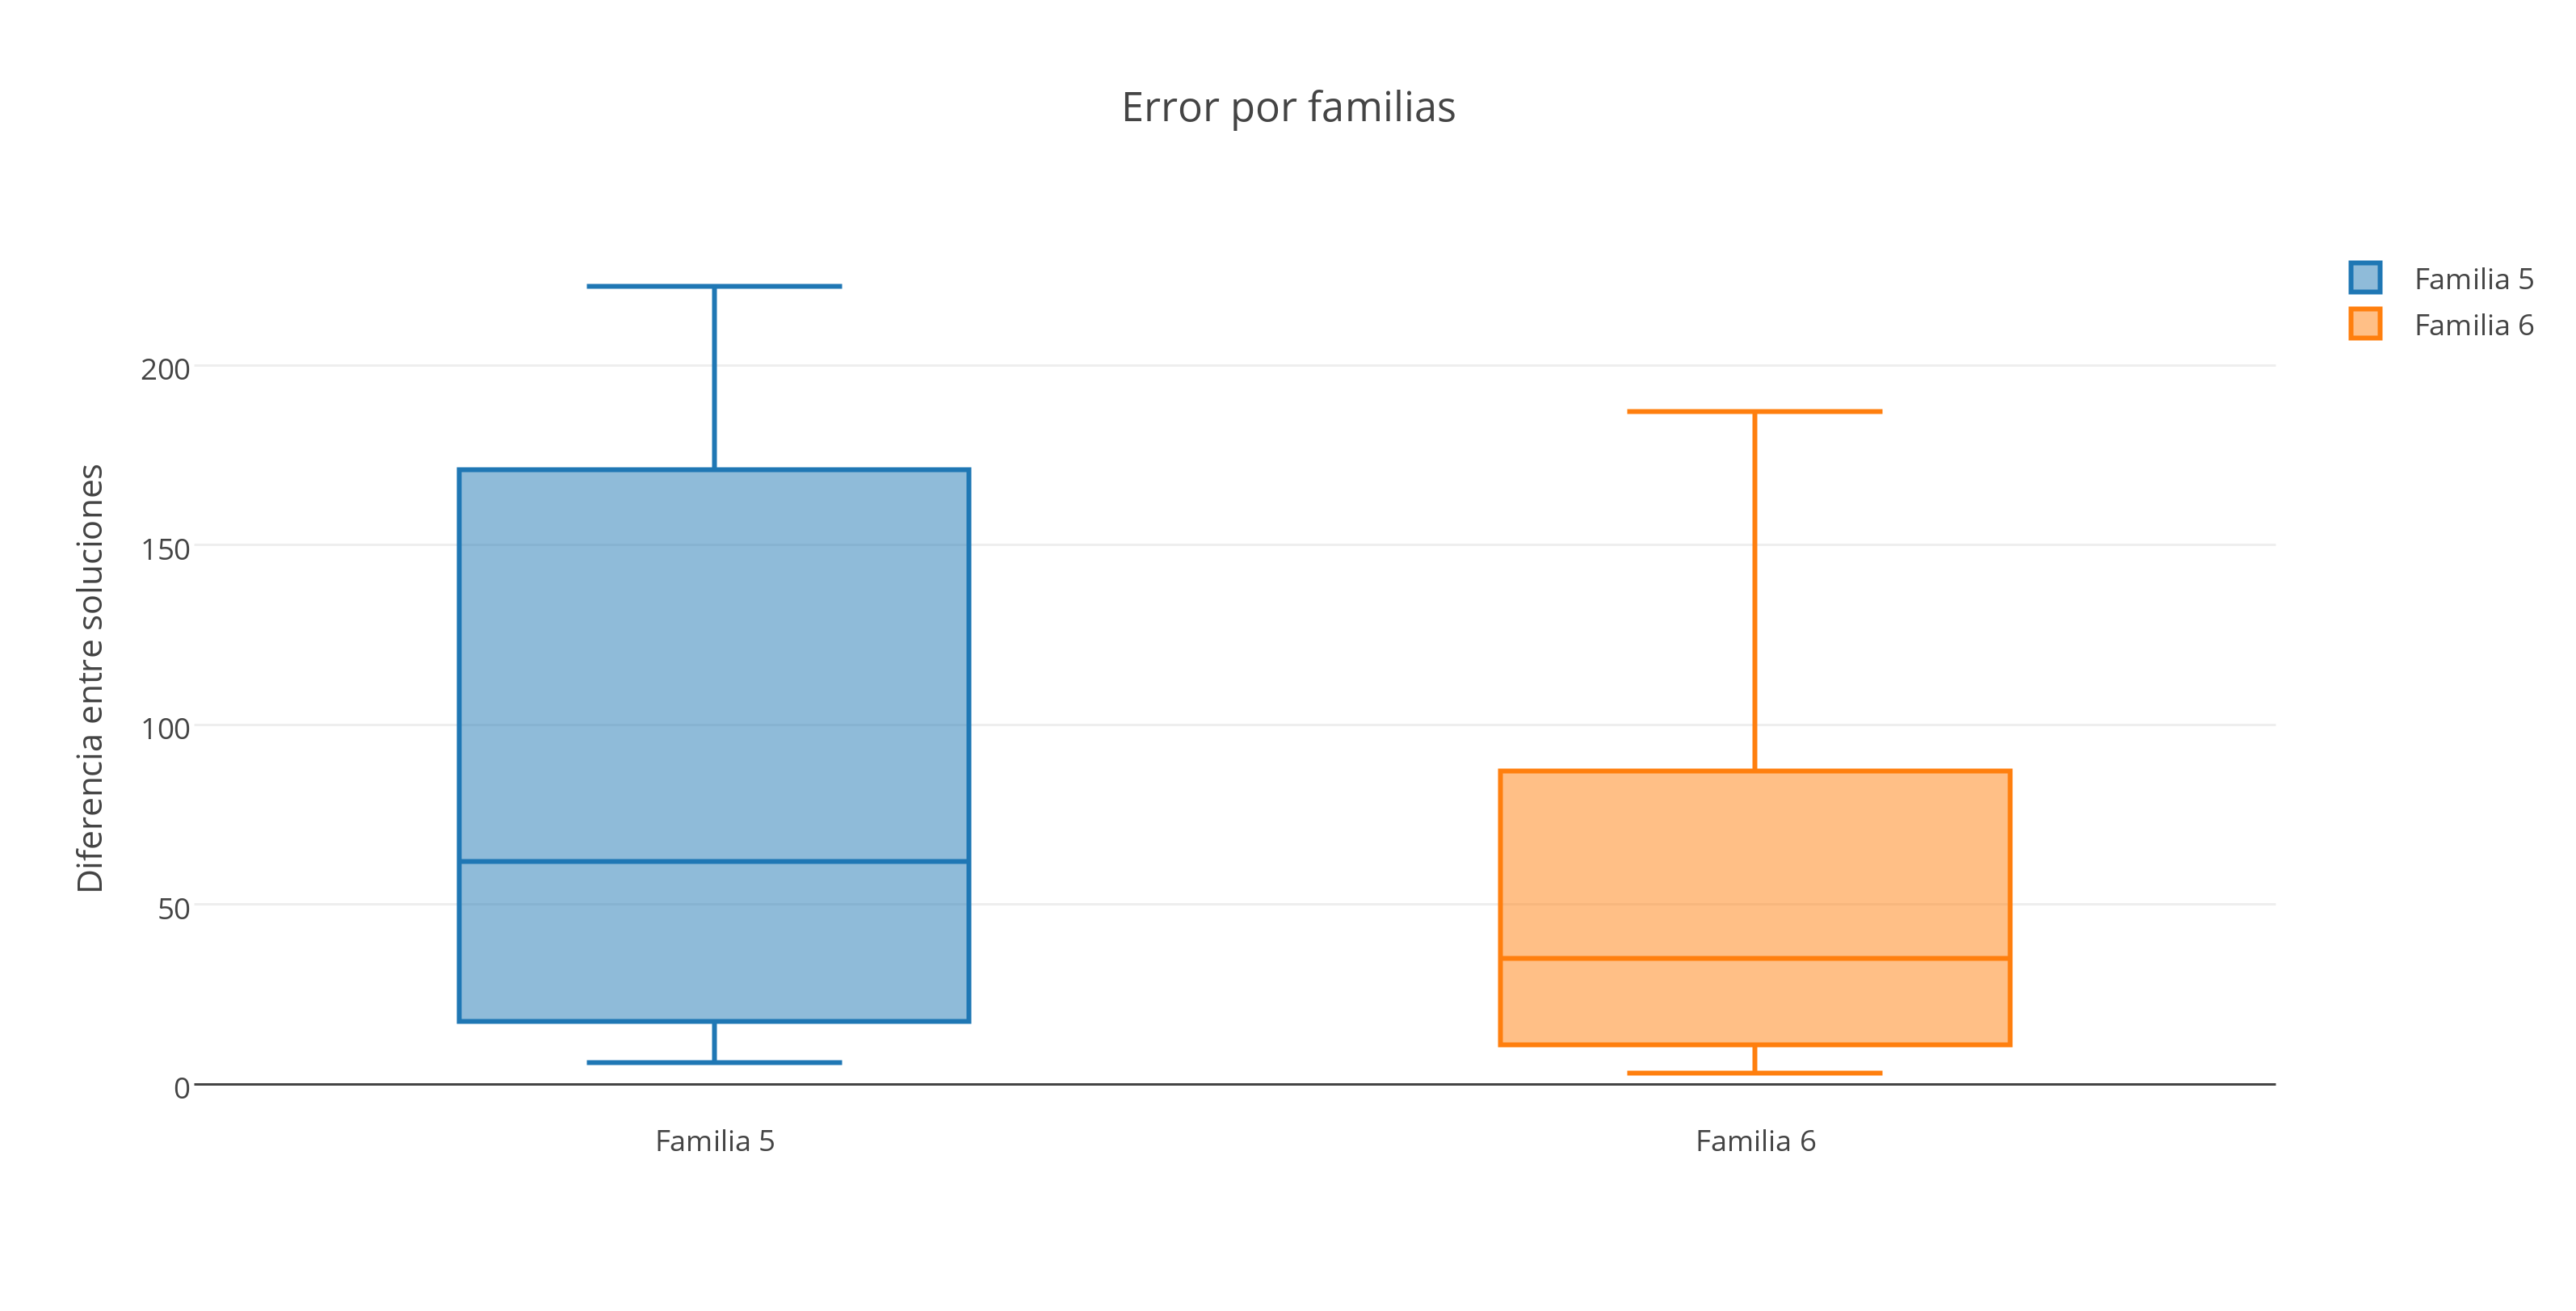
\includegraphics[width=0.75\textwidth]{./EJ2/box1.png}
\end{center}

\subsubsection*{Comparación entre tiempos de familias}

Veremos como se comporta cada familia en funci\'on del tiempo al ir aumentando la cantidad de elementos manteniendo las condiciones para que sigan perteneciendo cada uno a su respectiva familia.

\vspace*{0.3cm} \vspace*{0.3cm}
  \begin{center}
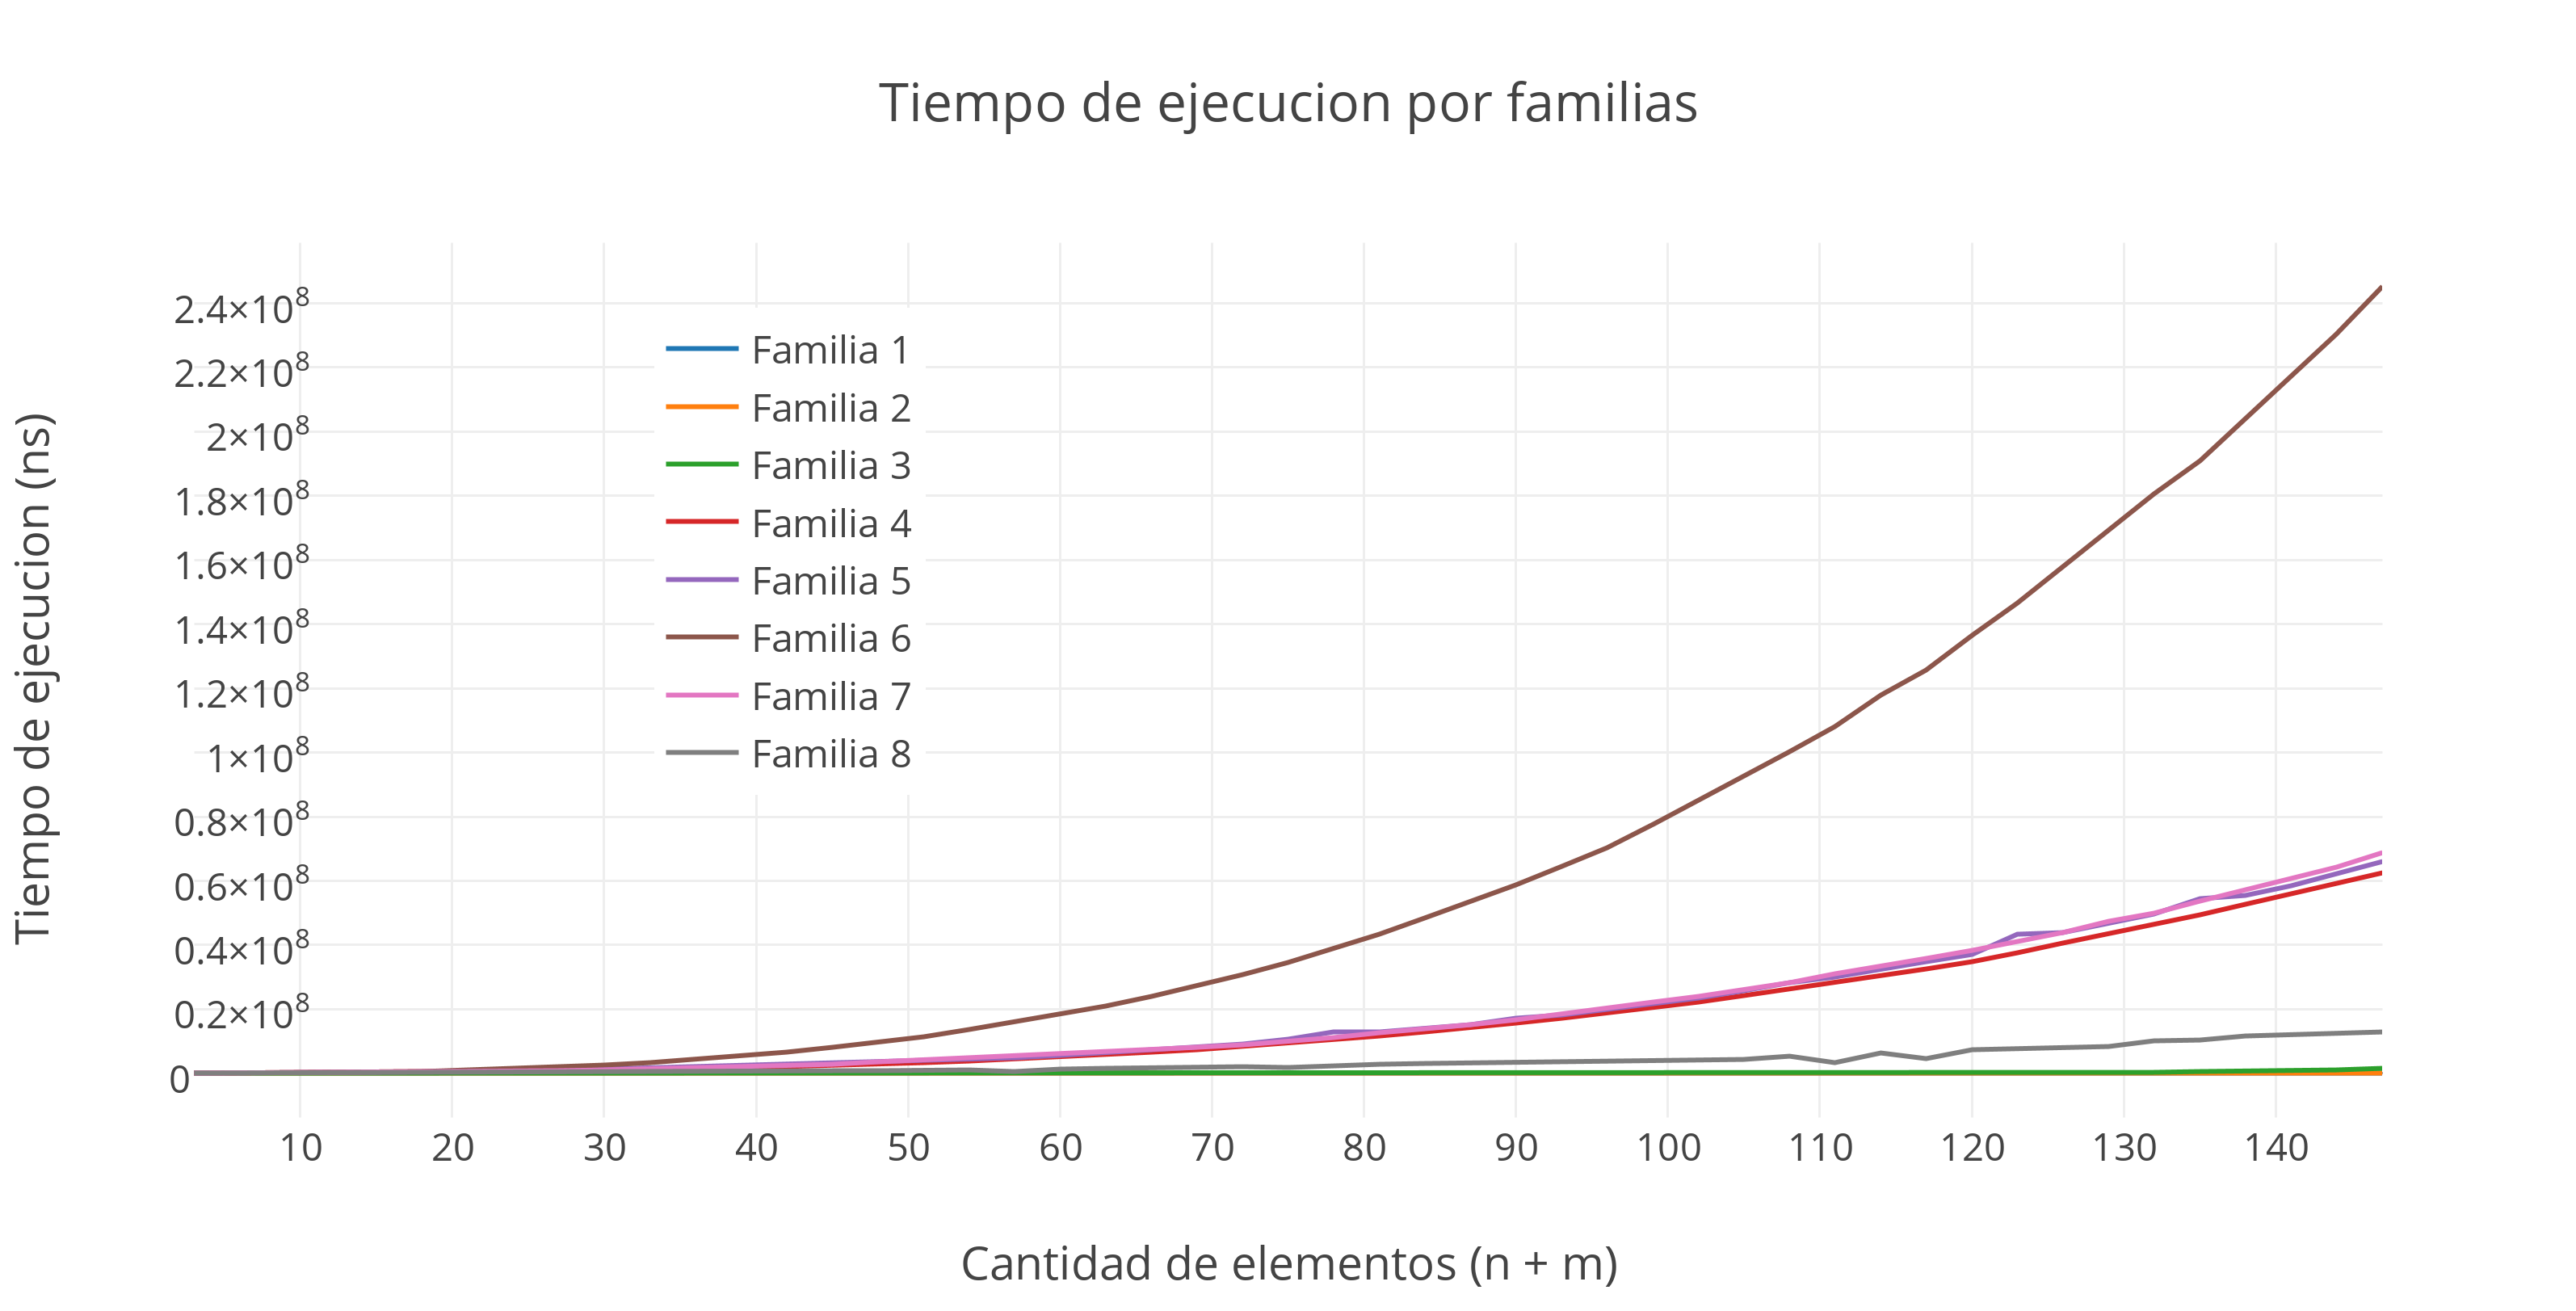
\includegraphics[scale=0.60]{./EJ2/comparativo.png}
\\{\textit{Tiempo de ejecución entre familias}}
  \end{center}
  \vspace*{0.3cm}
  \begin{figure} [!ht]
 \centering
  \subfloat[Detalle sin la familia 6]{
    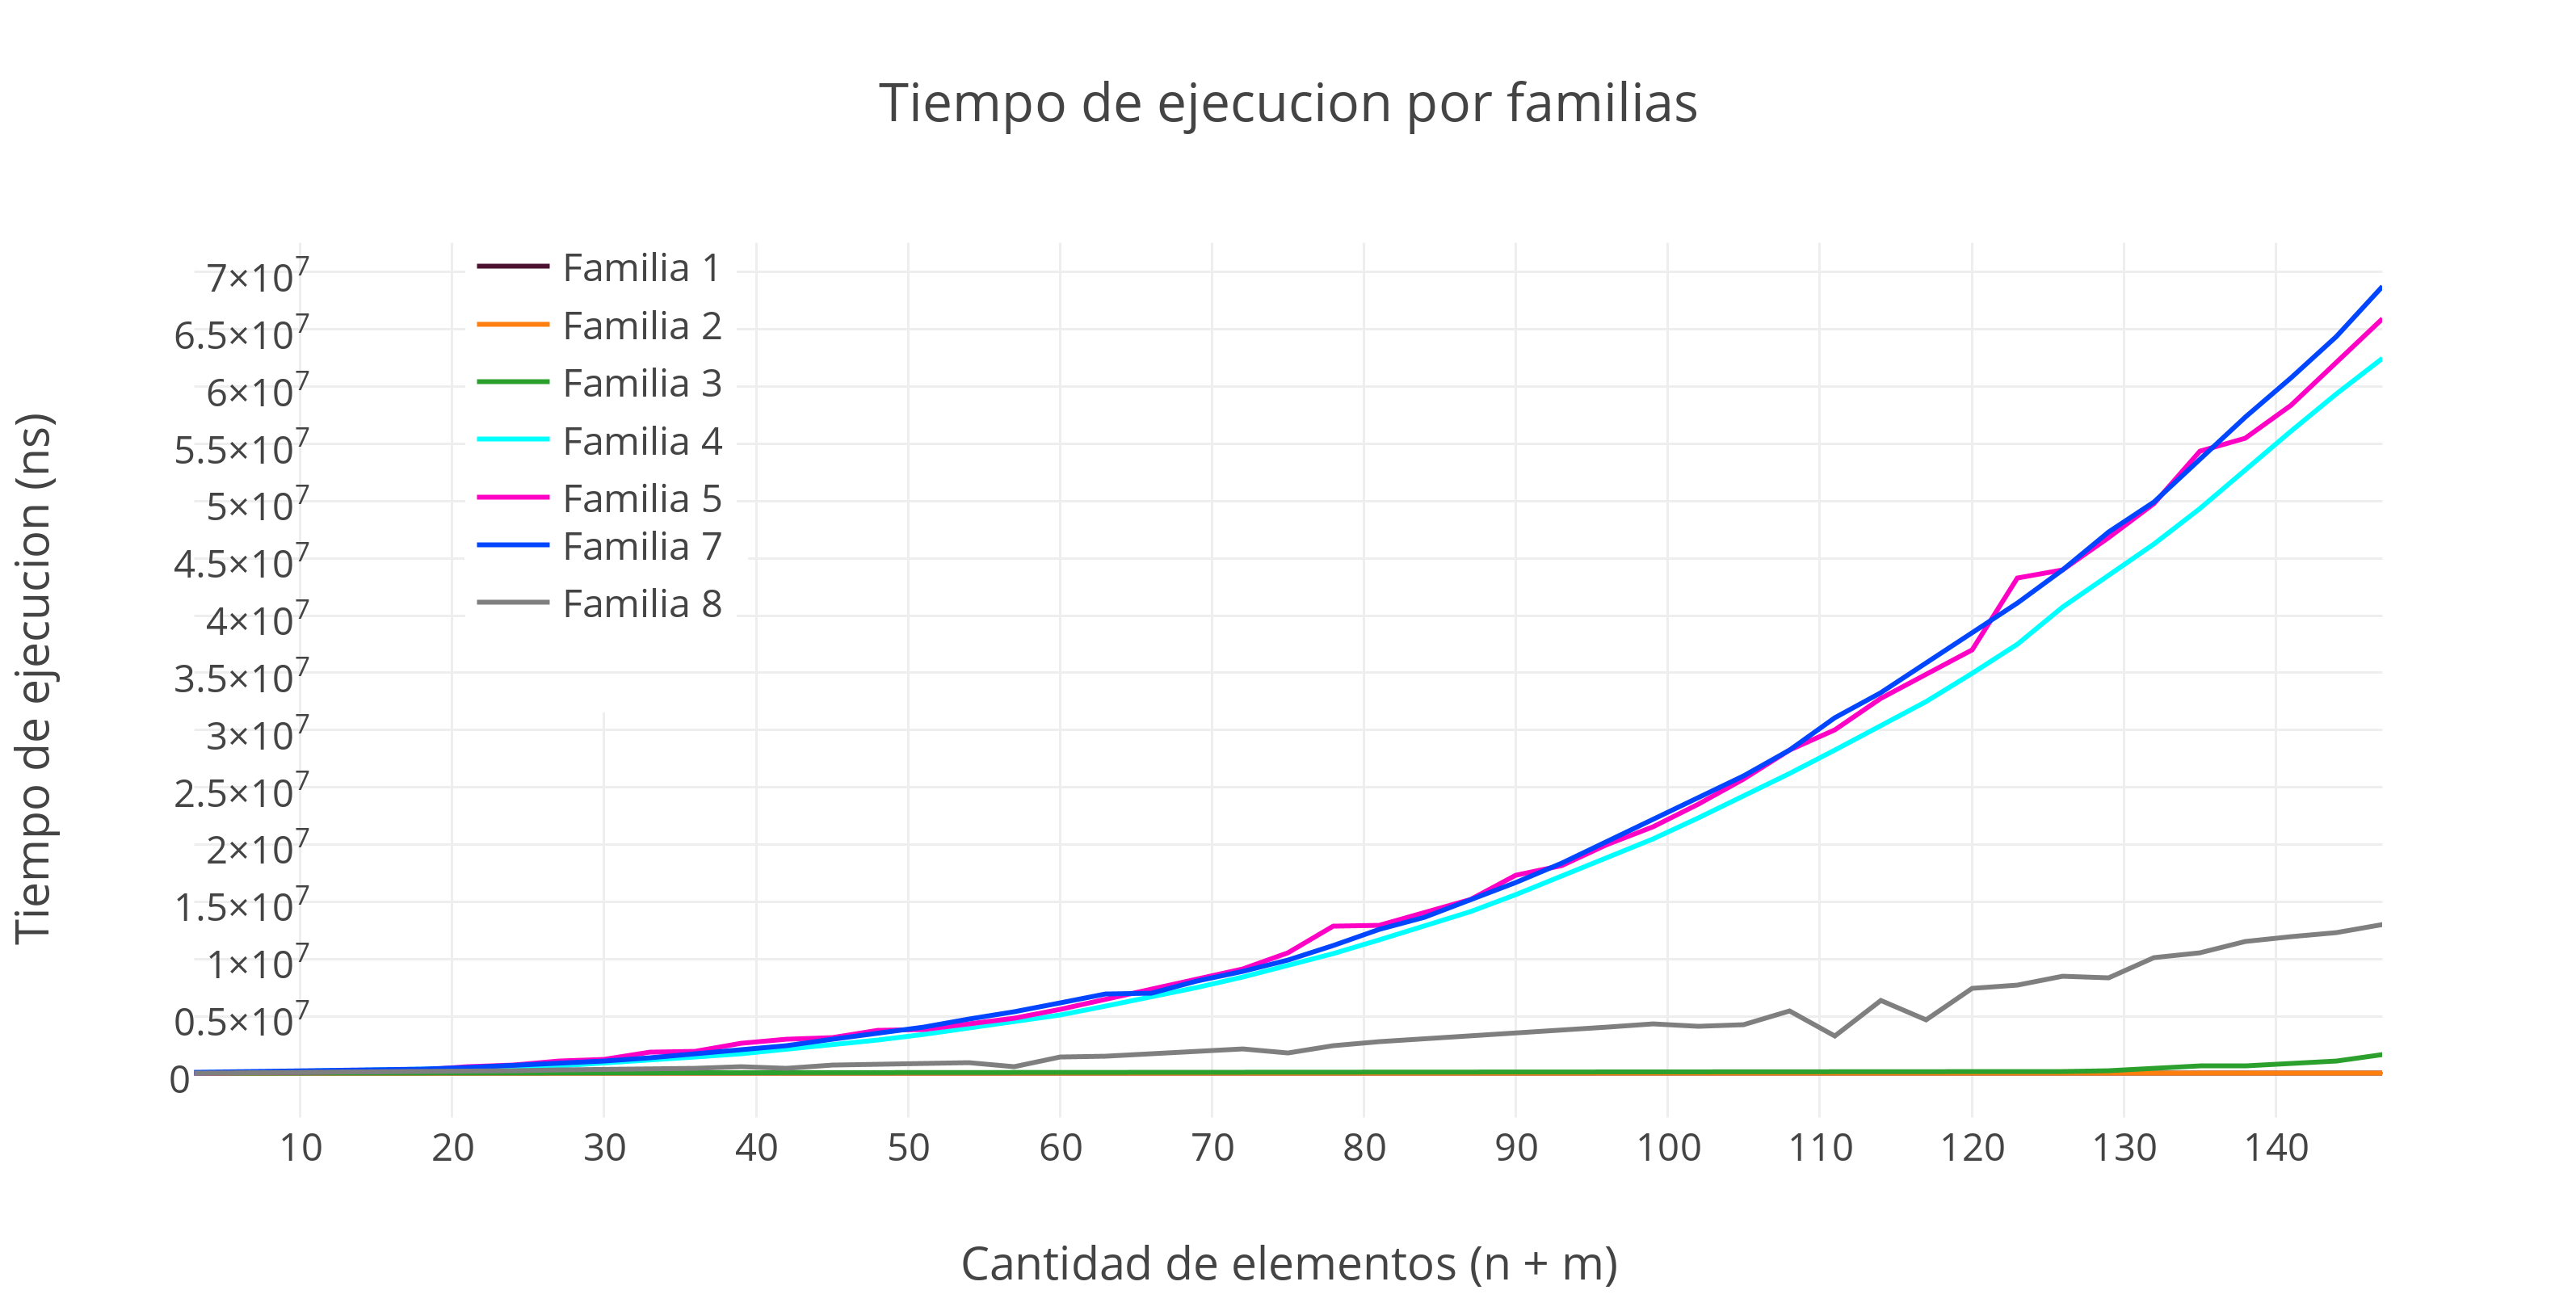
\includegraphics[width=0.45\textwidth]{./EJ2/comparativo1.png}}
    \label{fig:comparativo1}
  \subfloat[Detalle de las familias menos costosas]{
    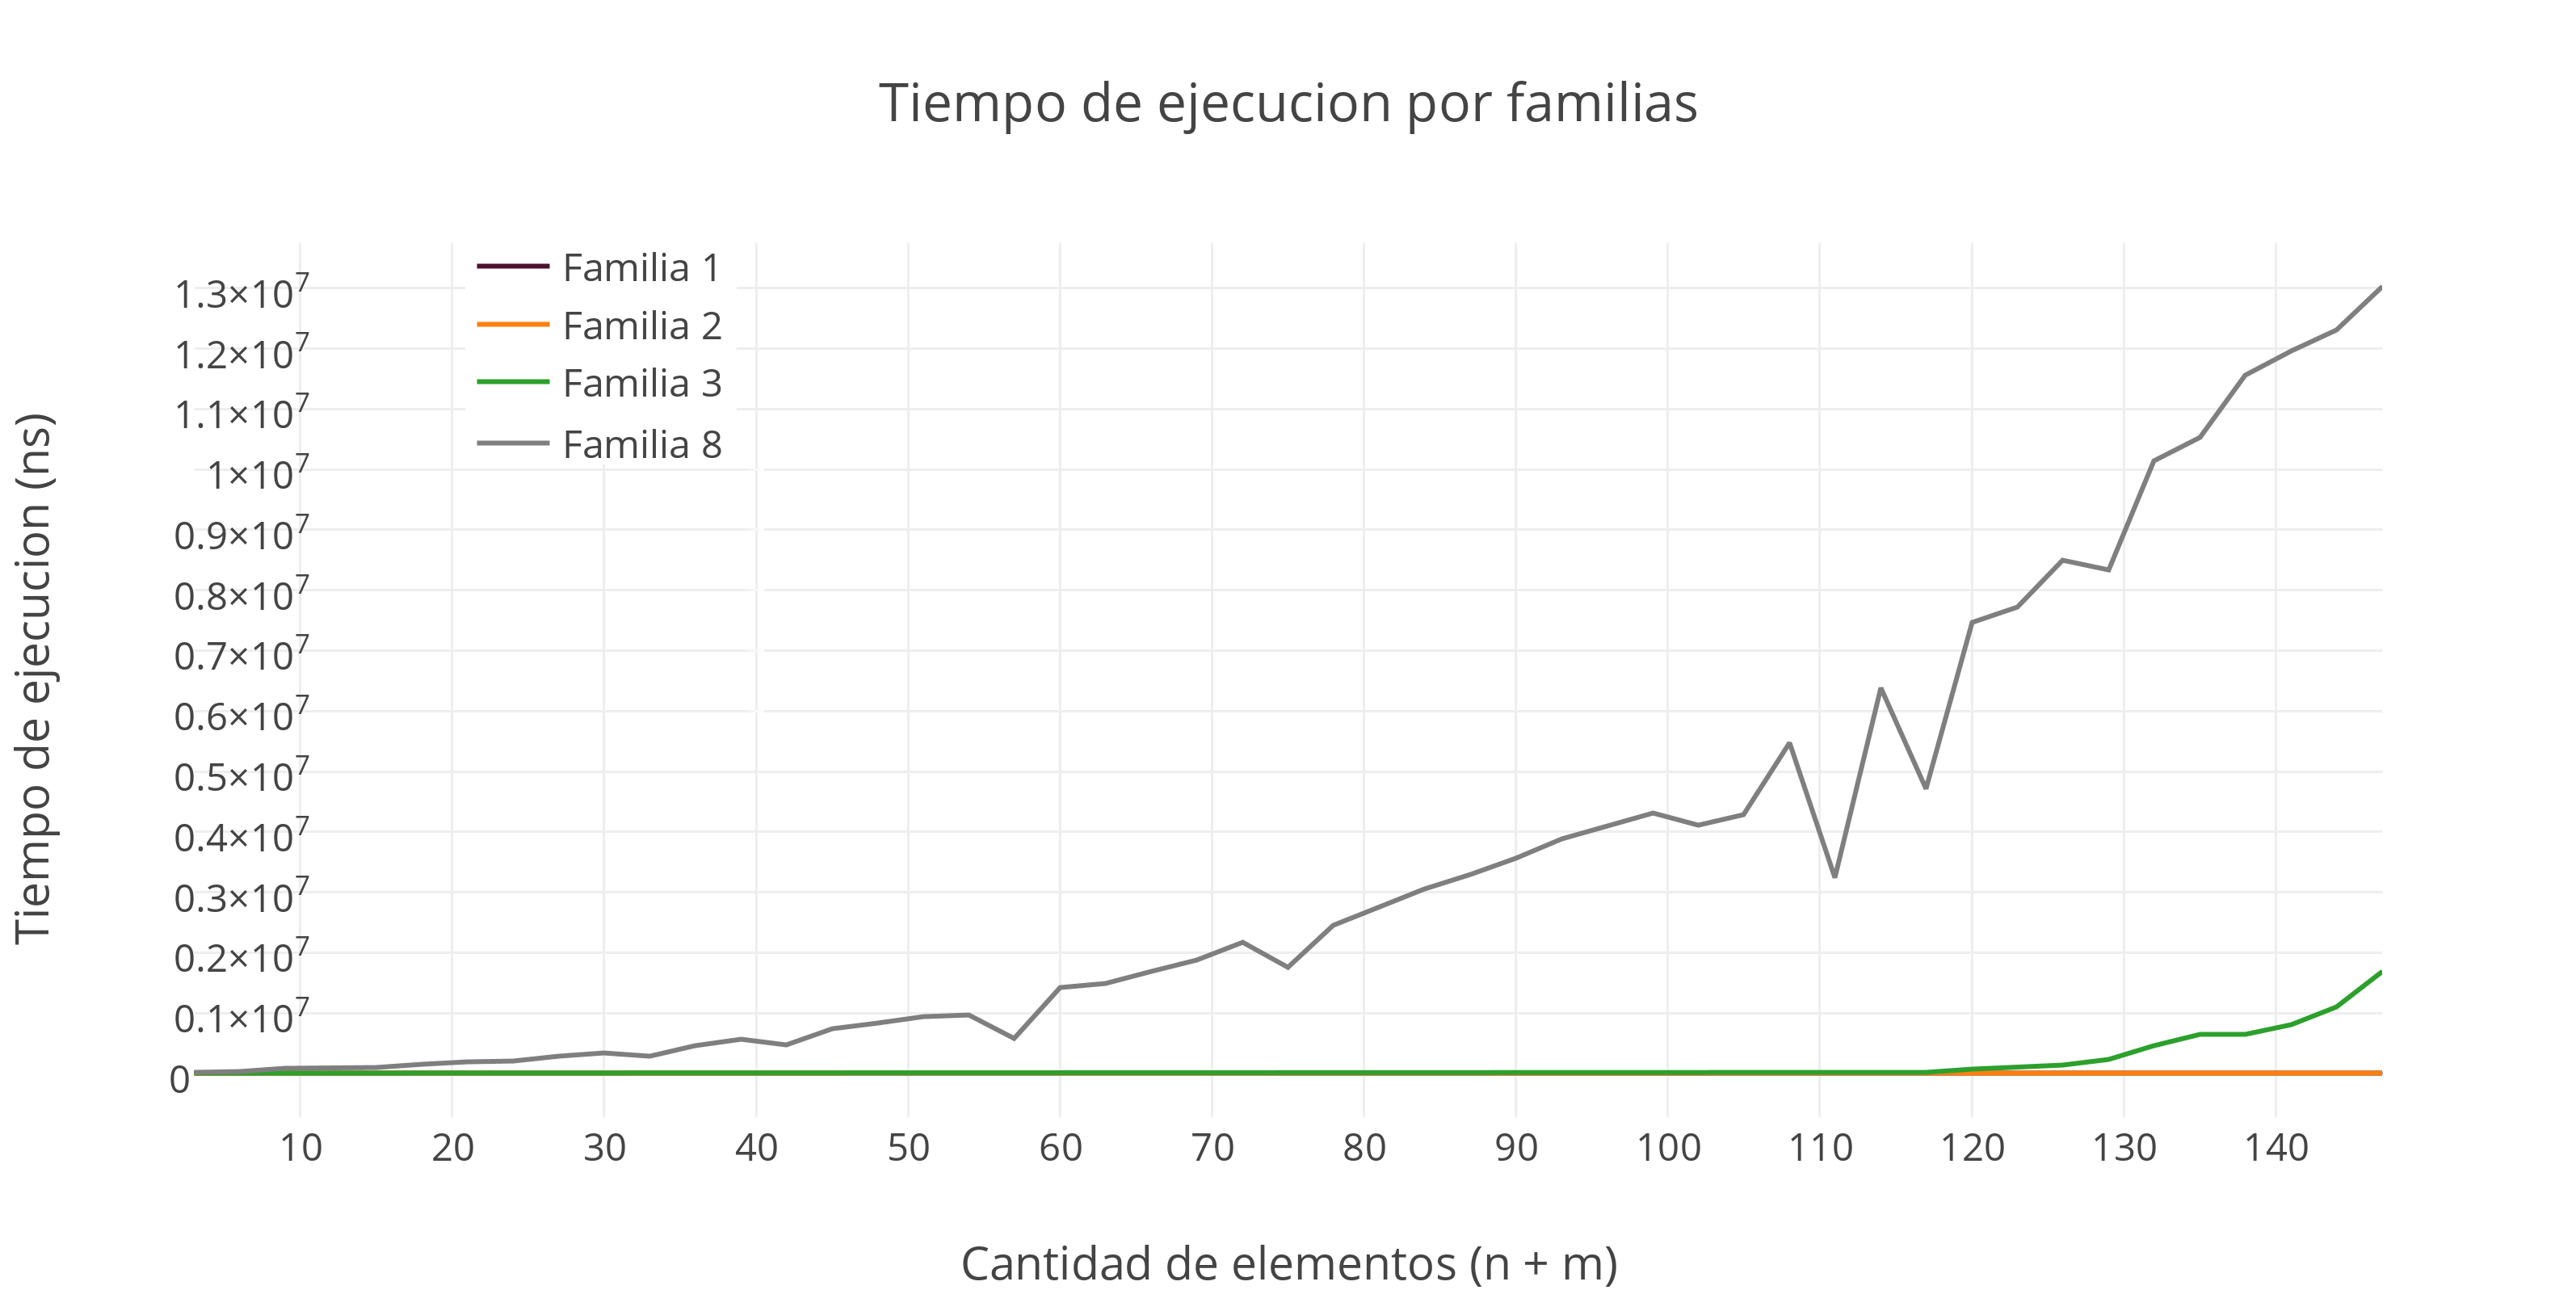
\includegraphics[width=0.45\textwidth]{./EJ2/comparativo2.png}}
    \label{fig:comparativo2}
    \end{figure}

Se puede observar como la familia n\'umero 6 presenta una peor performance en comparaci\'on al resto mientras que tanto la familia 1 como la 2 presentan un tiempo que se torna constante dando una mejor performance en relaci\'on al resto, lo cual se debe a las podas utilizadas para estas familias como mencionamos anteriormente. Mientras que la n\'umero 6 presenta la dificultad en la cual todos los elementos del mapa se encuentran desordenados, por lo tanto nuestro algoritmo tiene que llegar a hacer hasta un doble viaje para poder vencer a un gimnasio, ya que se dan instancias en las cuales los gimnasios de poder menor o igual a 3 se encuentran muy lejos de las pokeparadas en relaci\'on a los gimnasios de poder mayor, los cuales estan "pegados" a las pokeparadas insumiendo as\'i un tiempo mayor de decisi\'on y ejecuci\'on. Como hab\'iamos visto, nuestro algoritmo siempre que puede vencer a un gimnasio va a vencerlo.

Luego, mostraremos como se comporta nuestro algoritmo en base a la complejidad calculada anteriormente:

\vspace*{0.3cm} \vspace*{0.3cm}
  \begin{center}
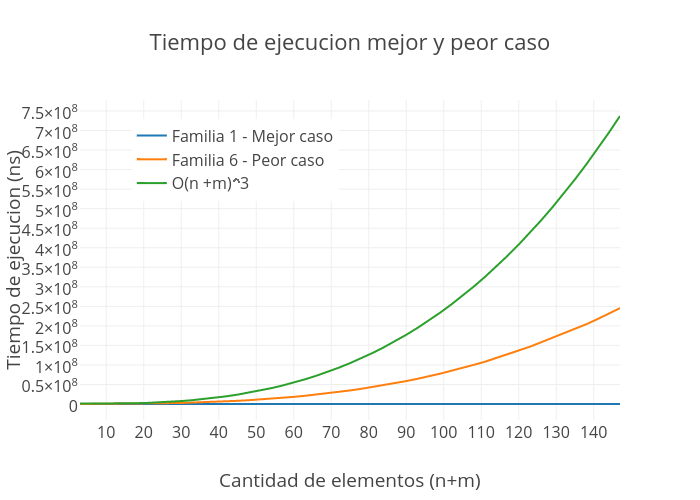
\includegraphics[scale=0.60]{./EJ2/mejorcaso.png}
\\{\textit{Tiempo de ejecución entre familias}}
  \end{center}
  \vspace*{0.3cm}

  
Es posible observar como las funciones resultantes del mejor y peor caso se encuentran por debajo de la cota de complejidad. Dicha complejidad fué calculada utilizando el m\'etodo de cuadrados m\'inimos generando una función que es tomada como cota dentro de nuestro orden de complejidad $(O(n+m)^3)$. 

\subsubsection*{Familias random y Gimnasios por grupos}

Como se comentó previamente en el ejercicio uno, las anteriores familias fueron de utilidad para analizar que sucede con el algoritmo goloso dado cierto tipo de entradas y porque no obtiene solución óptima en algunos casos, además de servir para analizar las podas tanto del algorito exacto como el goloso. Lo que no fué posible con estas familias es analizar que sucede en el promedio de casos con soluciones aleatorias, dado que eran familias totalmente controladas para poder observar particularidades. Por este motivo introducimos aquí dos familias nuevas con el objetivo de analizar casos promedio dentro de conjuntos de un cierto tamaño.\\

La primera es la familia Random, que como el nombre lo indica, todo es absolutamente random en los parámetros de entrada. Con este tipo de instancias podremos observar cual es el desempeño de los algoritmos en promedio.

La segunda familia también tiene parámetros aleatorios, pero organiza gimnasios por cuadrantes o grupos, donde $\forall$ $C_i$ con $i$ $\in$ ${1..4}$, todos los gimnasios en el cuadrante $C_j$ tienen el mismo poder. Otra regla que trató de aplicarse es que el poder de los gimnasios sea diferente para cada cuadrante $C_i$, $C_j$ con $i \neq j$. Esto será posible siempre y cuando no sea posible asignar m\'as de 1 (uno) de poder a los gimnasios, en cuyo caso, puede haber cuadrantes que tienen el mismo poder para sus gimnasios.

Esta familia será como una suerte de mapa por niveles. Veremos de esta manera como se desenvuelve sobre todo el algoritmo goloso para obtener un camino dentro de estas circunstancias.\\

Para el caso del valor de la mochila, con más de 15 elementos solo se analizará tomando el mínimo de mochila posible, y hasta con 15 elementos, podremos comparar contra el exacto que resulta de tomar la peor o la mejor mochila.
La mochila mínima será el valor del gimnasio con más poder más un extra de 3 ya que si el gimnasio más poderoso tiene valor menor a 3 podría generarse un caso sin solución. La mochila más grande será la suma de los poderes de todos los gimnasios. Mochilas con mayor tamaño harán que sobre capacidad.\\

Con respecto a la creación de casos para cada familia se idearon dos rangos iniciales:

\begin{itemize}
\item Rango 1: de 5 a 15 elementos. Por cada instancia de tamaño $n$ se tomaron $n*5$ instancias aleatorias.
\item Rango 2: desde 70 hasta 470 elementos en intervalos de 50 elementos. Por cada instancia de tamaño $n$ se tomó un 50\% del tamaño de la entrada. 
\end{itemize}

La cantidad de intancias dentro de cada tamaño será utilizada para promediar distancias y tiempos. En el caso del Rango 1 podremos calcular el error relativo de la solución del algoritmo goloso contra el exacto.\\

El calculo del error relativo se realiza tomando el promedio de todas las distancias obtenidas por el backtraking y el promedio de todas las distancias de las soluciones del algoritmo goloso para instancias del mismo tamaño. Sean $promedio_{exacto}$ y $promedio_{greedy}$ los valores respectivos, el error relativo se calcula como:

\begin{equation}
Error_{abs} = |promedio_{greedy}-promedio_{exacto}|
\end{equation}
\begin{equation}
Error_{rel} = \frac{Error_{abs}}{promedio_{exacto}} \ast 100
\end{equation}

La idea del Rango 1 era poder calcular hasta con 20 elementos utilizando backtracking, pero debido a los elevados tiempos de resolución se fué achicando el tamaño de las instancias hasta 15 elementos. La cantidad de instancias tomadas por cada tamaño permite obtener promedios más consistentes para que las comparaciones contra el backtracking sean de la mejor calidad posible y puedan aportar información relevante.

Dentro del Rango 2 los intervalos de 50 elementos podrían parecer ser demasiado, pero cuanto más se discretiza más tiempo de espera se necesita para correr todos los algoritmos que se verán en este informe. Como el objetivo principal es observar que sucede a medida que la entrada crece, se priorizó testear casos grandes resignando discretización.
El 50\% como elección en la cantidad de ejemplos tomados en cada tamaño fué suficiente para obtener resultados consistentes y mantener controlados los tiempos de experientación.

\newpage   

\subsubsection*{Repercusi\'on del tamaño de la mochila: hasta 15 elementos (pokeparadas + gimnasios)}

Se realizaron dos experimentas en base a la familia Random y a Gimnasios por grupos para ver como repercute el tamaño enunciado, con la mochila denominada grande y la chica. Luego de dicha experimentación, se desarrollaron los siguientes gr\'aficos en los cuales se puede observar como la heur\'istica golosa no presenta cambios en su soluci\'on al tener una mochila más grande, mientr\'as que el backtraking al tener una mochila con mayor capacidad logra obtener un camino diferente y de menor longitud.\\

\vspace*{0.3cm} \vspace*{0.3cm}
  \begin{center}
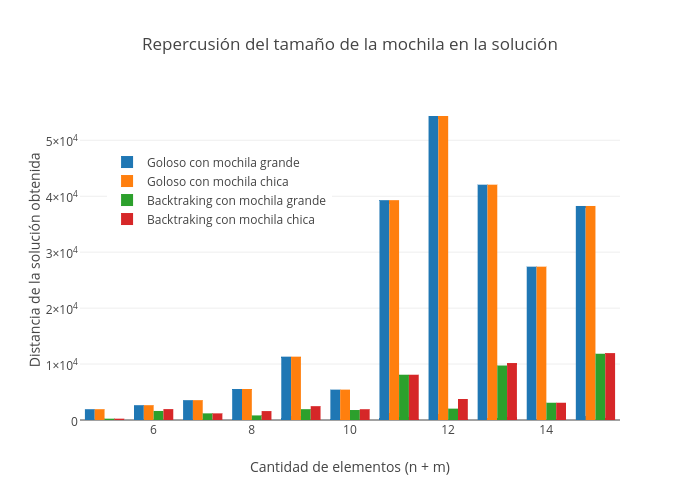
\includegraphics[scale=0.60]{./EJ2/familiaMochila.png}
\\{\textit{Gimnasios por grupos}}
  \end{center}
  \vspace*{0.3cm}
  \begin{figure} [h]
 \centering
  \subfloat[Repercusión en goloso]{
    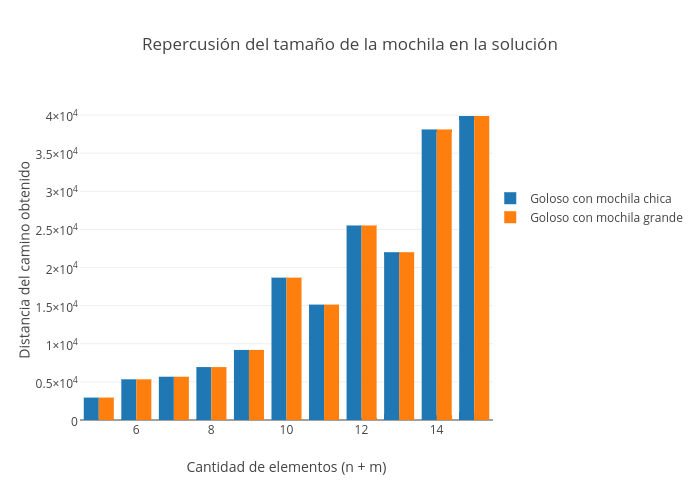
\includegraphics[width=0.45\textwidth]{./EJ2/familiaGoloso.png}}
    \label{fig:comparativo1}
  \subfloat[Repercusión en backtraking]{
    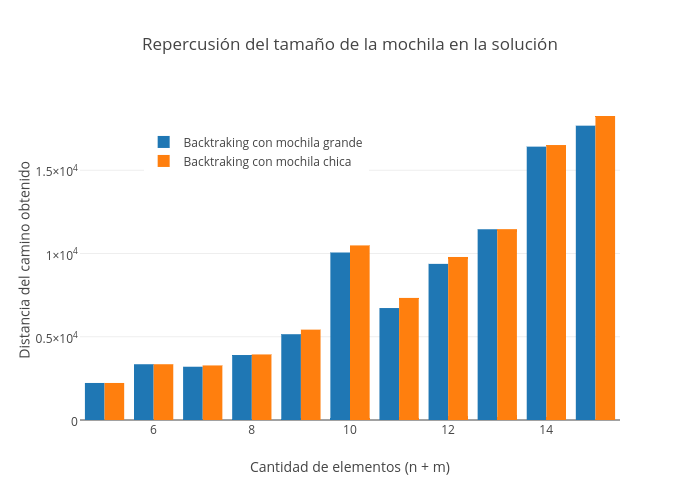
\includegraphics[width=0.45\textwidth]{./EJ2/familiaBack.png}}
    \label{fig:comparativo2}
    \end{figure}
  
\vspace*{0.3cm} \vspace*{0.3cm}
  \begin{center}
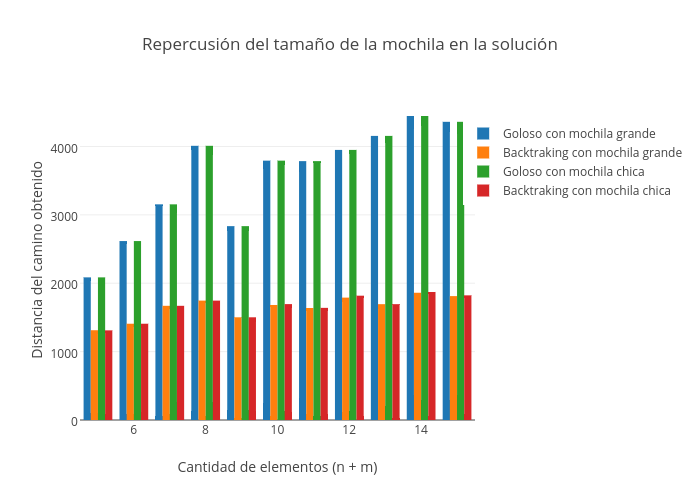
\includegraphics[scale=0.60]{./EJ2/randomMochila.png}
\\{\textit{Random}}
  \end{center}
  \vspace*{0.3cm}
  \begin{figure} [h]
 \centering
  \subfloat[Repercusión en goloso]{
    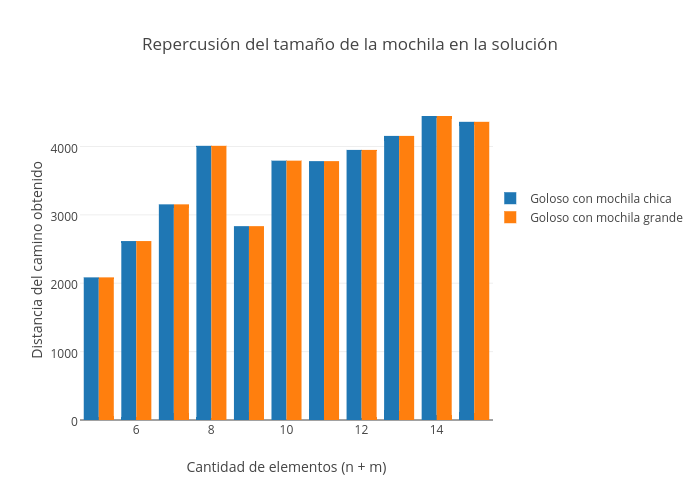
\includegraphics[width=0.45\textwidth]{./EJ2/randomGoloso.png}}
    \label{fig:comparativo1}
  \subfloat[Repercusión en backtraking]{
    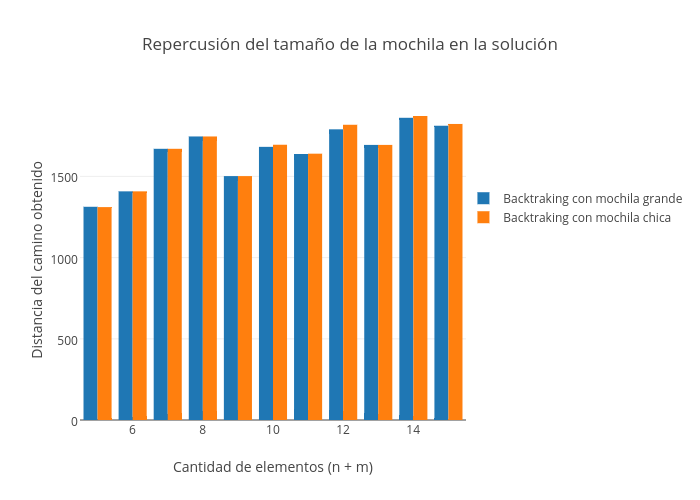
\includegraphics[width=0.45\textwidth]{./EJ2/randomBack.png}}
    \label{fig:comparativo2}
    \end{figure}
   

El motivo principal de que no haya cambios se debe a que siempre que existe la posibilidad de vencer a un gimnasio el algoritmo toma esa decisión. Podemos notar sin embargo, algunas mejorías en cuanto a las mochilas grandes para los resultados del backtracking. Siempre se podrá obtener un resultado exacto mejor si se dispone de más capacidad de carga. Si se dispone de las pokeparadas suficientes, con la mochila más grande posible podríamos primero cargar todas las pokeparadas necesarias y luego ir a vencer a todos los gimnasios. Si los gimnasios están lejos de todas las pokeparadas, esto termina beneficiando a la distancia recorrida ya que no será necesario volver a recargarse. 

\newpage

\subsubsection*{Repercusi\'on del tamaño de la mochila: más de 15 elementos}

Como se mencionó en repetidas oportunidades, al algoritmo goloso no saca partida de la capacidad de la mochila. Como con más de 15 elementos nos fué imposible calcular el backtracking en el ordenador disponible en tiempos razonables (más de 30 minutos para 16 elementos y era necesario correr al menos la mitad del tamaño en ejemplos para obtener promedios), no podremos comparar que sucede al utilizar la peor y mejor mochila contra el resultado exacto.

\subsubsection*{Comparación de bactracking y algoritmo goloso para la familia Random}

\begin{figure} [h]
 \centering
  \subfloat[Comparación solución golosa vs exacta]{
    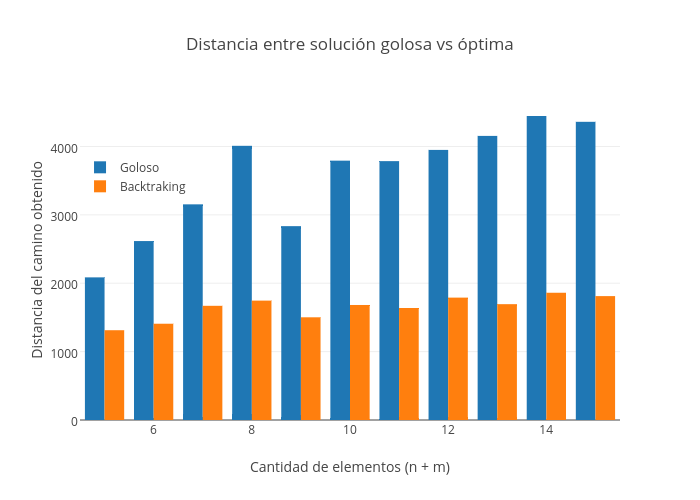
\includegraphics[width=0.45\textwidth]{./EJ2/random.png}}
       \label{fig:randomexacto}
  \subfloat[Error relativo]{
    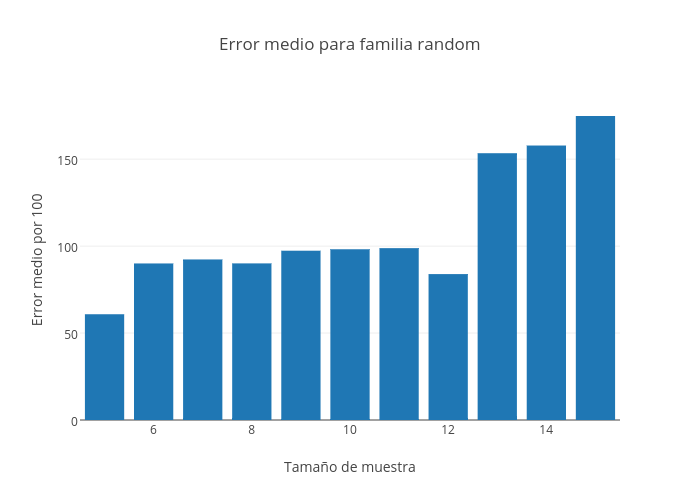
\includegraphics[width=0.45\textwidth]{./EJ2/randomError.png}}
    \label{fig:randomgoloso}
    \end{figure}
    
Según podemos observar en los gráficos, las distancias del algoritmo goloso tienden a crecer mientras que la solución exacta se mantiene. Dado que los tamaños son pequeños y la familia es totalmente aleatoria, es probable que para las instancias generadas suceda que las distancias de las soluciones óptimas varíe poco, pero el algoritmo goloso siempre tiende a empeorar la solución cuanto más grande es la instancia. Esto último se verá mejor luego con tamaños de entrada mayores a 15 elementos.

\subsubsection*{Comparación de bactracking y algoritmo goloso para la familia de Gimnasios por grupos} 

   \begin{figure}[h]
 \centering
  \subfloat[Comparación solución golosa vs exacta]{
    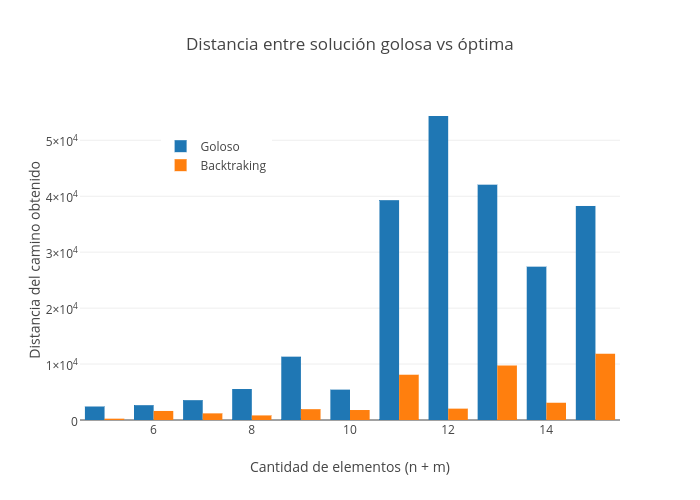
\includegraphics[width=0.45\textwidth]{./EJ2/familia.png}}
       \label{fig:randomexacto}
  \subfloat[Error relativo]{
    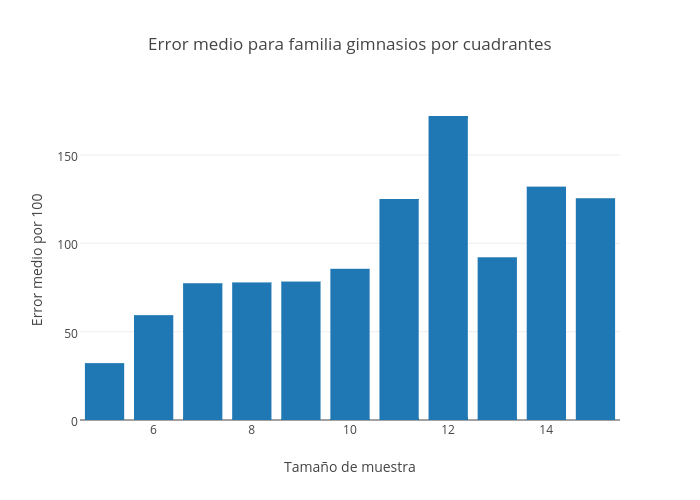
\includegraphics[width=0.45\textwidth]{./EJ2/familiaError.png}}
    \label{fig:randomgoloso}
    \end{figure}

Se observa para esta familia un error considerable cuanto más grande es la instancia, llegando a estar por arriba del 100\% con respecto al resultado exacto para entradas de más de 11 elementos. El motivo lo atribuimos a la caracteristica de grupos que disponen los gimnasios. Es decir, la mayoría de las veces se recorren grandes distancias para vencer a un gimnasio luego de juntar pokeparadas. Esto último podría suceder al menos de dos formas; grupos de gimnasios densos que hacen que haya pocas pokeparadas entre ellos y grupos de gimnasios alejados de pokeparadas. En cualquier caso, se obliga al goloso a recorrer más distancia para obtener el poder suficiente para vencer al proximo gimnasio.\\

En estos experimentos se evidencia lo malo que puede ser la elección golosa. Dado que el metodo goloso está restringido a la evaluación de un conjunto determinado de caminos, es posible que ignore los que minimizan el recorrido total. Esta ignorancia lleva, como en el caso estudiado, a una solución cada vez más alejada de la óptima (alcanzada por el backtraking) en las 15 dimensiones de instancias evaluadas.

%\subsection{Experimientos y conclusiones}
%\subsubsection[2.5]{Test}
%\indent Por medio de los tests dados por la c\'atedra, desarrollamos nuestros tests,
para corroborar que nuestro algoritmo era el indicado.\\

Dichos tests los hemos catalogado y diferenciado en distintos casos, que enunciaremos a continuación:

\begin{center}
 \textbf{Los portales alcanzan para cubrir todo el camino sin necesidad de caminar por los pasillos}
\end{center}
 Para este tipo de testeo mostraremos a continuaci\'on un ejemplo del mismo, exponiendo su respectivo resultado.\\

 \begin{center}
 \textbf{Necesidad de caminar por todo el pasillo para llegar hasta los portales}
\end{center}
 Como ejemplo mostraremos, exponiendo su respectivo resultado, el siguiente testeo.\\



%\subsubsection[2.5]{Performance del algoritmo}
%\indent En los siguientes tests queremos observar que sucede con cada familia de casos al ir variando los parámetros de entrada F, C de manera creciente y lineal y tomando los tiempos de corrida de cada input para poder compararlos.\\
Se comienza, por lo tanto, con una entrada de F*C = N y se la hace crecer en $n$ filas y columnas en cada instancia, por lo tanto cada familia crece linealmente. De manera que no hay desigualdades y todas las familias se miden en instancias de igual tamaño e igual cantidad de paredes.\\

Para obtener dichas instancias se realizaron aproximadamente unas 20 corridas con el mismo input y se tom\'o el promedio de esas 20 corridas en cada instancia para obtener un valor m\'as cercano a la media.\\ 

\textit{---> 20 corridas ? no fueron mas?!!! PREGUNTA SERIA: LOS PARAMETROS AUMETAN LINEALMENTE EN LOS TESTS? ESO ES RE IMPORTANTE SI QUEREMOS ALGO CON UNA MEJOR FORMA}\\

Se pueden observar en el  gráfico 2.1, cinco funciones, que representan el tiempo de ejecuci\'on de las familias de casos mencionadas en el apartado anterior:\\

\begin{enumerate}
\item No existe arbol que conecte todas las salas
\item Existe un camino que conecta todas las salas de esfuerzo 0
\item El AGM es todo el grafo
\item Sin ejes
\item Camino por las salas random
\end{enumerate}

\vspace*{0.3cm} \vspace*{0.3cm}
  \begin{center}
 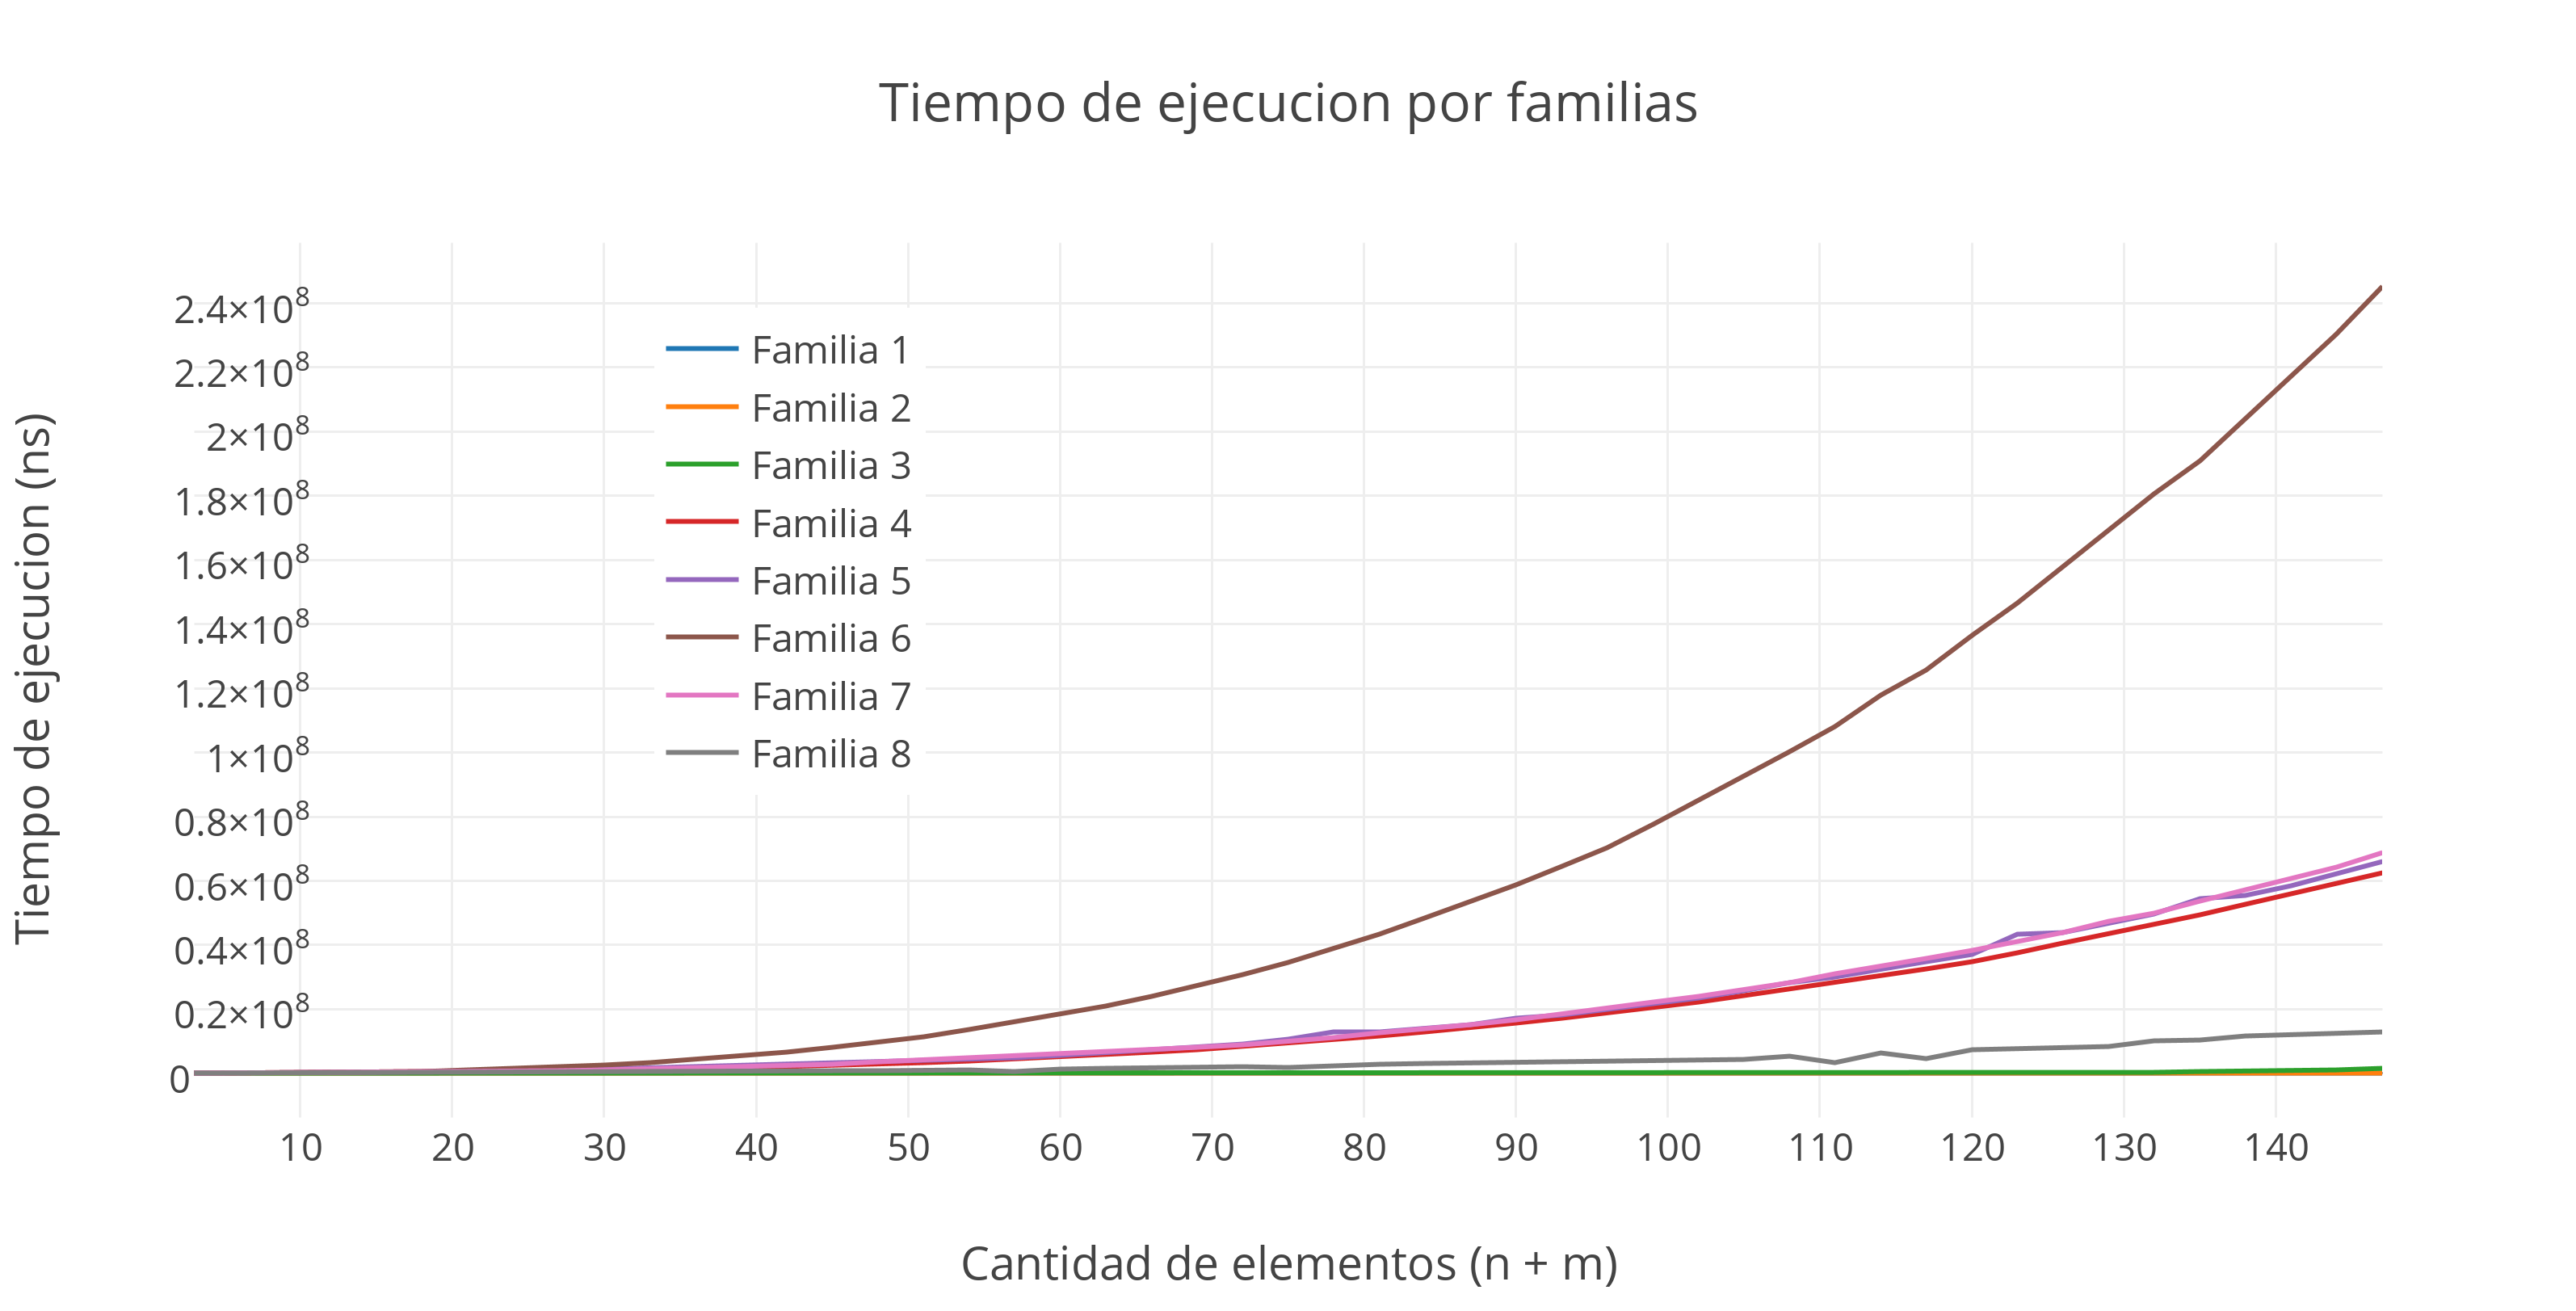
\includegraphics[scale=0.65]{./EJ2/comparativo.png}
 {$Gr$\'a$fico$ \ 2.1 - $Comparativo$}
  \end{center}
  \vspace*{0.3cm}
 
\textit{---> VER GRAFICO: REHACER. OJO LAS ETIQUETAS DEL GRAFICO, LA COMPLEJIDAD NO IRIA}\\

Como se observa en el gr\'afico la funci\'on representativa de la familia 4, presenta una mejor performance en relaci\'on a las otras. Esto se debe a que nuestro algoritmo al intentar chequear las aristas, observa que no hay ninguna y finaliza su ejecuci\'on insumiendo en tiempo unicamente la creaci\'on del grafo (nodos aislados)

Habiendo chequeado dichas instancias, llegamos a la conclusi\'on que la familia de casos que presenta una mejor performance para nuestro algoritmo
es la número 4 "\textbf{No existe arbol que conecte todas las salas}" dado que el grafo que se obtiene de transformar el laberinto recibido como par\'ametro no presenta ninguna arista.\\

Un grafo representativo de esta familia ser\'ia el siguiente:

\vspace*{0.3cm} \vspace*{0.3cm}
  \begin{center}
 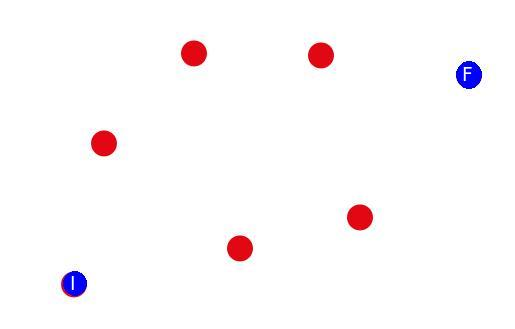
\includegraphics[scale=0.5]{./EJ2/grafoSinEjes.jpeg}
 \\{$Grafo$ \ 2.1 - $Mejor$ $Caso$}
  \end{center}
  \vspace*{0.3cm}

Verificando el peor caso en el gráfico 2.1, llegamos a la conclusi\'on que la familia de casos que hace que el algoritmo tenga más tiempo de computo ser\'a la familia 2 "\textbf{Existe un camino que conecta todas las salas de esfuerzo 0}" dado que el grafo que se obtiene de transformar el laberinto de entrada es aquel que presenta un ciclo por cada habitaci\'on posible, dandonos el siguiente grafo una vez transformado:\\

\vspace*{0.3cm} \vspace*{0.3cm}
  \begin{center}
 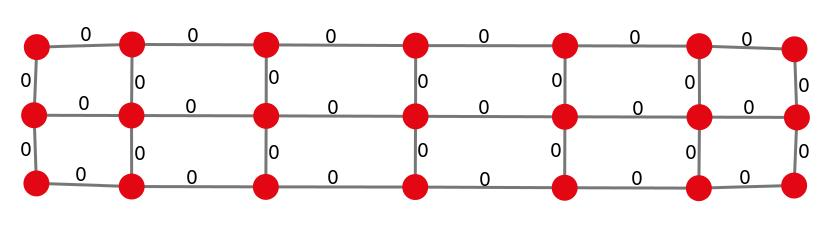
\includegraphics[scale=0.5]{./EJ2/ej2grafosinpared.jpeg}
 \\{$Grafo$ \ 2.2 - $Peor$ $Caso$}
  \end{center}
  \vspace*{0.3cm}
  
\textit{---> habria que explicar un poco que pasa en los otros casos!!!}\\
  
Veamos en detalle como se comportan el mejor y peor caso con respecto a la complejidad teorica calculada.\\

\vspace*{0.3cm} \vspace*{0.3cm}
  \begin{center}
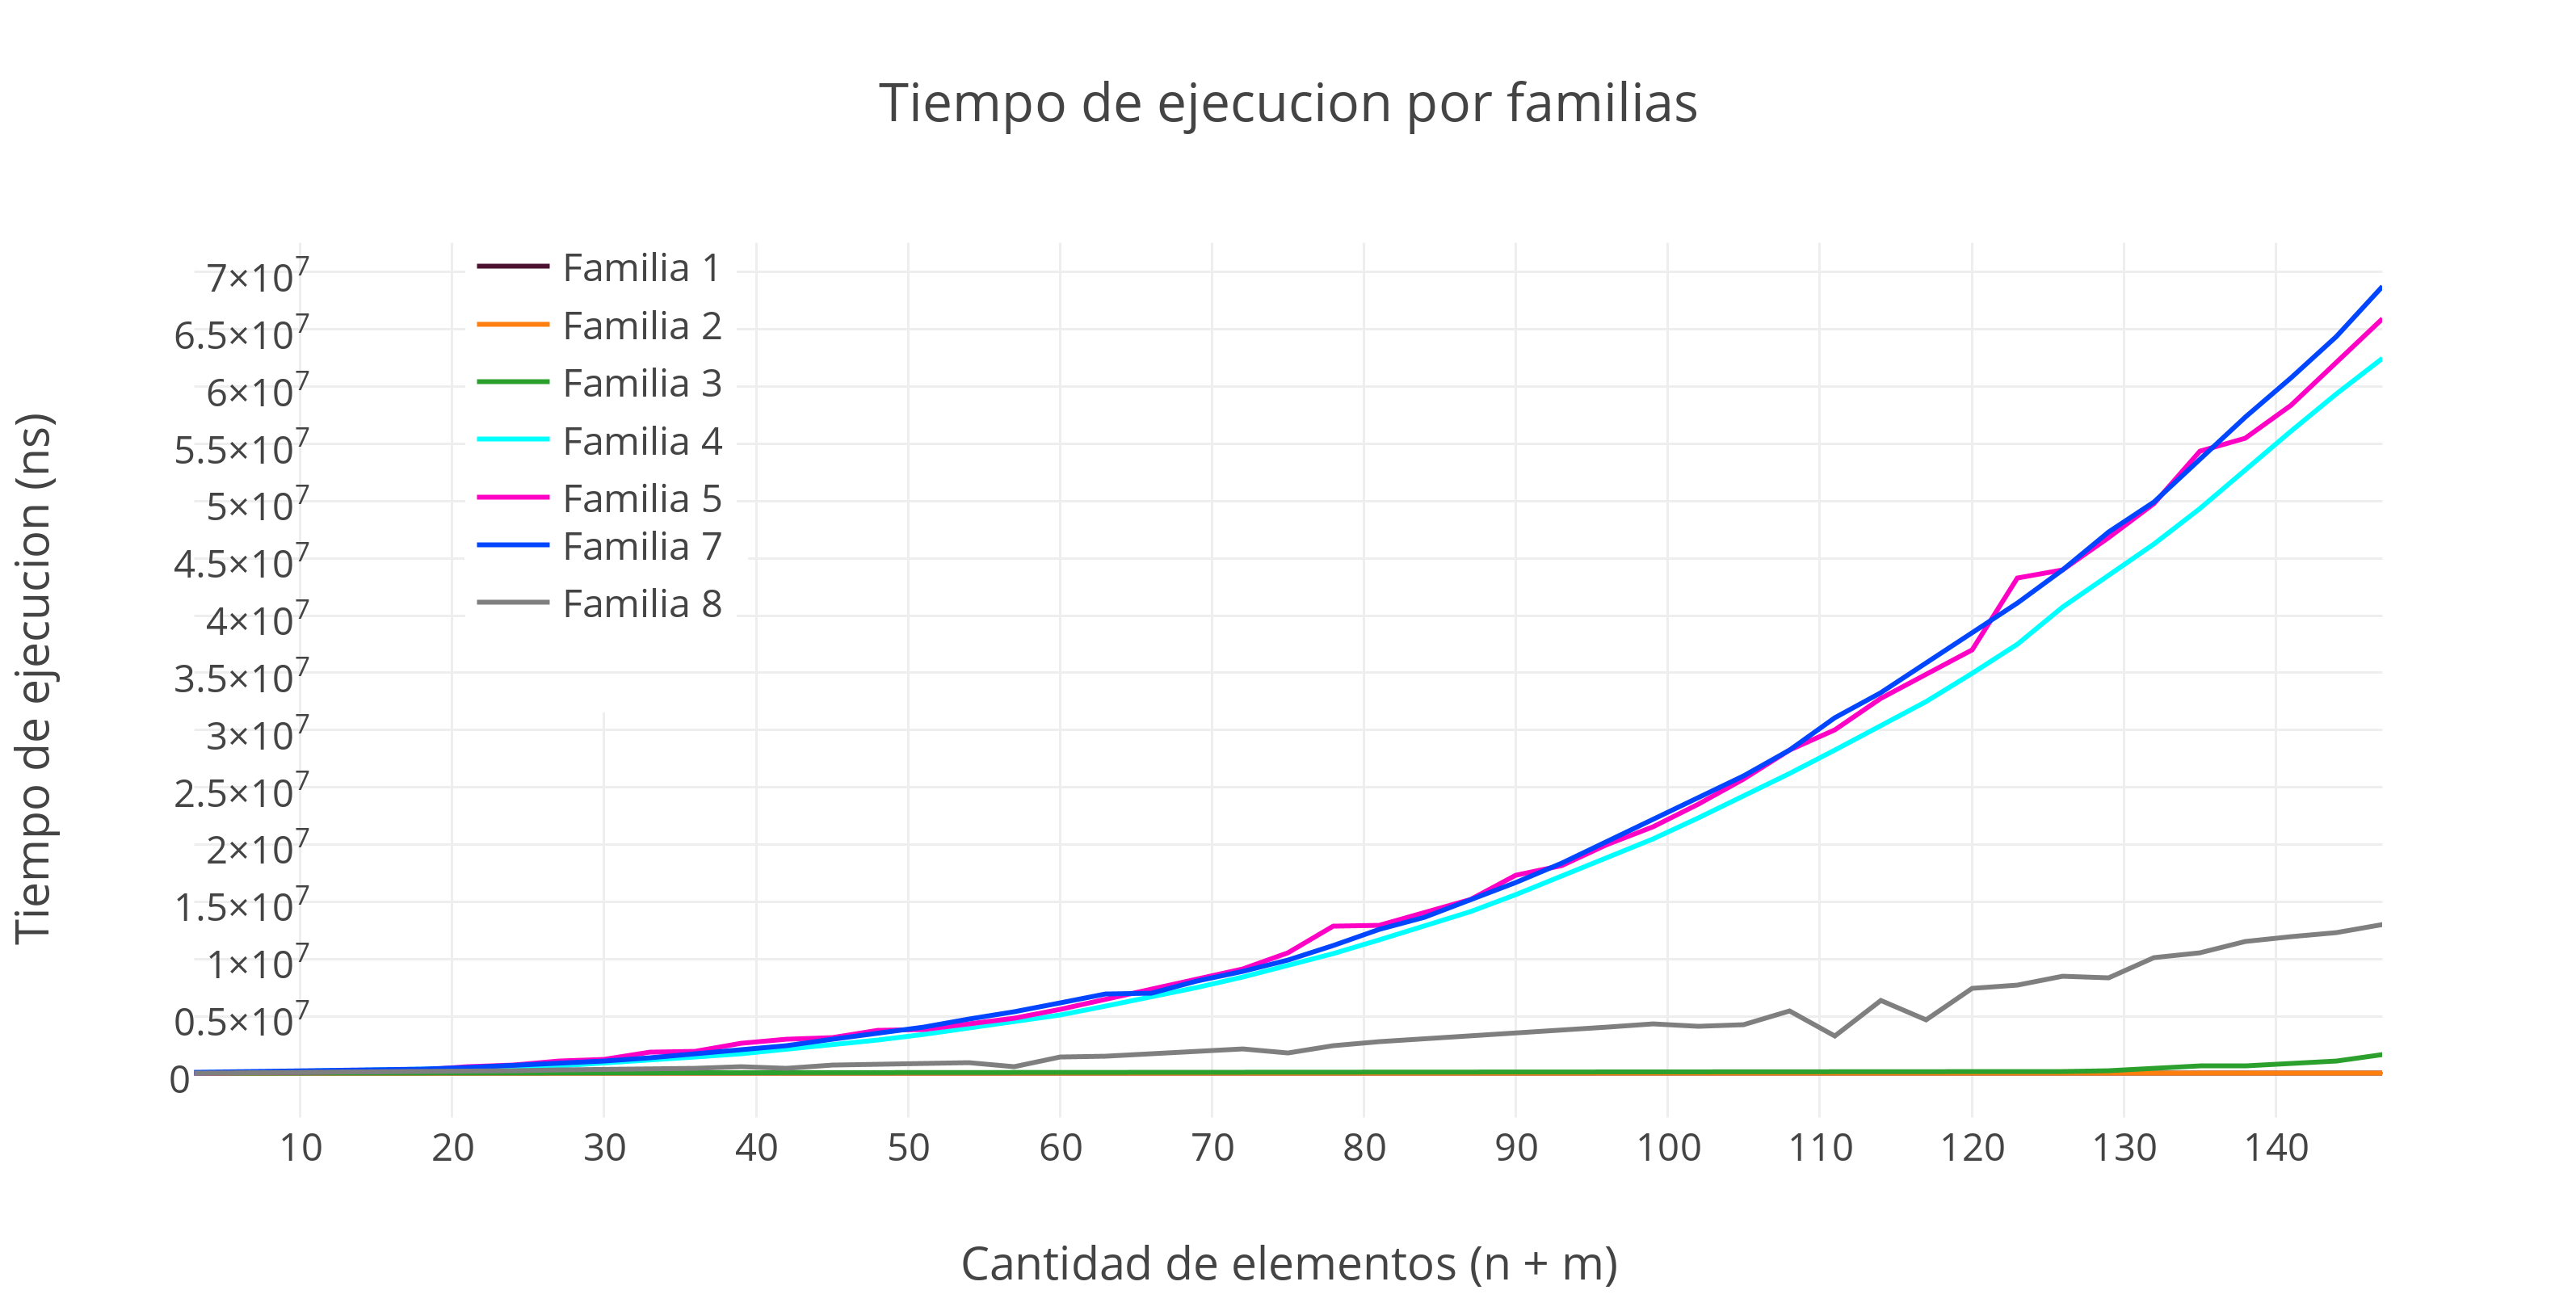
\includegraphics[scale=0.65]{./EJ2/comparativo1.png}
 {$Gr$\'a$fico$ \ 2.5 - $Comparativo$}
  \end{center}
  \vspace*{0.3cm}
  
\textit{---> VER GRAFICO: ESTE NO ES EL COMPARATIVO DE MEJOR Y PEOR. OJO LAS ETIQUETAS DEL GRAFICO, LA COMPLEJIDAD LA FITEAMOS}\\  
  
Podemos ver en este gr\'afico comparativo como las familias est\'an acotadas por la funci\'on de la complejidad te\'orica calculada.\\

\textit{---> Cuando retestiemos, vamos a fitear esto con nuestra complejidad, que no se como es, luego tenemos que hacer alguna conclusion. Deberia ser algo cuadratica.}\\
  
Luego de dichos experimentos y casos probados, se puede concluir que a pesar de tener ciclos en todas las salas y donde dichos ciclos presenten aristas con pesos iguales lo que genera al algoritmo la posibilidad de crear varias ramas posibles de soluci\'on los tiempos se mantienen dentro de la complejidad propuesta.\\


\newpage
\section{Ejercicio 3} 
\subsection{Explicaci\'on de resoluci\'on del problema}
%La soluci\'on planteada utiliza la t\'ecnica algor\'itmica de \textit{backtracking}. La idea es %recorrer todas las configuraciones posibles manteniendo la mejor soluci\'on encontrada hasta el momento. 

%Inicialmente, ordenaremos en base al peso y el valor de todos los objetos.\\
%Luego de realizar esto iremos agregando en las mochilas los objetos de mayor valor teniendo en cuenta el peso de los mismos con la mochila, en caso de que al agregar un objeto la suma de los pesos de los objetos que se encuentran en la mochila diera igual o mayor al peso m\'aximo de la mochila, se quitar\'a el objeto ultimo y se probar\'a con otro objeto de menor peso.\\
%As\'i realizaremos todas las posibles permutaciones de objetos en la mochila.\\
%Una vez que obtuvimos todas las permutaciones posibles nos quedaremos con la m\'axima, de esta manera tendr\'iamos en las mochilas una cantidad \'ptima de objetos con el mayor valor posible y un peso acorde a lo soportado por las mochilas.\\


%Las solucion planteada se basa en una generalización del problema de la mochila extendida a las 3 mochilas indicadas en la cota dada por la consigna.\\
\subsubsection*{Obteniendo el valor máximo}
 El problema de la mochila analiza, para cada objeto, el máximo valor que se puede obtener para cada capacidad posible de la mochila.Si llamamos K a la capacidad de la mochila, se evaluara introducir   el elemento suponiendo capacidad $k_{i}$ para i = 1, 2,..., hasta K. En cada evaluación se decide entre no meter el elemento, con lo cual el valor máximo de la mochila que tenga la capacidad $k_{i}$ será el calculado con algun elemento anterior (o cero en el caso de que sea el primero en ser evaluado); o meter el elemento, con lo cual, al valor del elemento se le suma el valor de la mochila de capacidad K - $k_{i}$ que sea máxima. De esta forma, se genera un subproblema que respeta el principio de optimalidad, con lo cual se puede aplicar programación dinámica para solucionar el problema. \\
 
  Extendiendonos a 2 mochilas, al evaluar la $k_{i}$ posibilidad de la primer mochila (con capacidad $K_{a}$), se debe tener en cuenta que tambien está la posibilidad de utilizar la segunda mochila (con capacidad $K_{b}$). Esto nos muestra que por cada elemento debemos calcular $K_{a} \times K_{b}$ combinaciones de capacidades. Sin contar el primer elemento, el resto calculara sus combinaciones en base a las del elemento que le precedió en la evaluación, siguiendo la idea del algoritmo original de una mochila. Para obtener el valor final, se buscará en la matriz resultante de evaluar el último elemento, a la combinación de capacidades entre ambas mochilas que resulte máxima.\\
  
  Con la misma lógica podemos ver que para 3 mochilas donde se tienen capacidades  $K_{a}$,$K_{b}$ y $K_{c}$, cada elemento disponible evaluará $K_{a} \times K_{b} \times K_{c}$ posibilidades. En este caso se buscará la solución en la matriz tridimensionál de posibilidades obtenidas del último elemento evaluado.

\subsubsection*{Recuperando los elementos utilizados}

Siendo que la consigna pide los objetos involucrados en la solución, es necesaria una forma de, a partir de los valores máximos obtenidos, deducir los elementos que fueron usados y el lugar donde fueron colocados para lograr el resultado.\\

Analizando la última matriz del caso de 2 mochilas (sin perder generalización para 3 mochilas), podemos notar que por cada objeto que iteramos para intentar encontrarle un lugar en las mochilas, deja el valor previo, de cada combinacion de capacidades, sin tocar cuando el objeto no es utilizado. Al ser utilizado, se cambia el valor por el nuevo máximo alcanzado. De utilizar 1 matriz solamente, y actualizarla por cada objeto, se perderá la posibilidad de saber si se usó o no a cada uno, ya que no se tendrá un "paso anterior" por haber sido reescrito en cada paso subsiguiente. \\

Para recuperar estos estados, se resuelve guardar la matriz involucrada en el calculo de cada elemento.
\subsection{Pseudoc\'odigo}
\begin{algorithm}[H] %or another one check
 \Fn{swap()}{
 %     \SetAlgoLined
   $S_o$ es la solución que brinda el algoritmo goloso \\
  	n es cantidad de nodos de $S_o$ \\
  	$S_{actual}$ $\leftarrow$ $S_o$ \hfill O(n)\\
  	entero costoAnterior $\leftarrow$ calcularCosto($S_o$) \hfill O(1)\\
  	$S_{final}$ $\leftarrow$ $S_o$ \hfill O(n)\\
	\For{i de 1 a n}{ 
		\hfill ciclo: O(n)\\	
		\For{j de 1 a n}{ 
		\hfill ciclo: O(n)\\	
			 $intercambiar$ $posiciones$ i con j en $S_{actual}$ \hfill O(1)\\
			 optimizarS($S_{actual}$) \hfill O(n)\\
			 entero costoActual $\leftarrow$ calcularCosto($S_{actual}$) \hfill O(n)\\
			 \If{costoActual $<>$ -1 $\wedge$ costoActual < costoAnterior}{
			 	costoAnterior $\leftarrow$ costoActual \hfill O(1)\\
			 	$S_{final}$ $\leftarrow$ $S_{actual}$ \hfill O(n)\\
			 }
			 $intercambiar$ $posiciones$ i con j en $S_{actual}$ \hfill O(1)\\	 		
		}	
	}
	
	devolver $S_{final}$ \\	
	
	\hfill complejidad total: O($n^3$)\\			
}
\end{algorithm}

\begin{algorithm}[H] %or another one check
 \Fn{2opt()}{
 %     \SetAlgoLined
   $S_o$ es la solución que brinda el algoritmo goloso \\
  	n es cantidad de nodos de $S_o$ \\
  	$S_{actual}$ $\leftarrow$ $S_o$ \hfill O(n)\\
  	entero costoAnterior $\leftarrow$ calcularCosto($S_o$) \hfill O(1)\\
  	$S_{final}$ = $S_o$ \hfill O(n)\\
	\For{i de 1 a n}{
	\hfill ciclo: O(n)\\
		\For{j de i+1 a n}{
		\hfill ciclo: O(n)\\
			 $invertir$ $rango$ de i a j en $S_{actual}$ \hfill O(n)\\
			 optimizarS($S_{actual}$) \hfill O(n)\\
			 entero costoActual $\leftarrow$ calcularCosto($S_{actual}$) \hfill O(n)\\
			 \If{costoActual $<>$ -1 $\wedge$ costoActual < costoAnterior}{
			 	costoAnterior $\leftarrow$ costoActual \hfill O(1)\\
			 	$S_{final}$ $\leftarrow$ $S_{actual}$ \hfill O(n)\\
			 }
			 $invertir$ $rango$ de i a j en $S_{actual}$ \hfill O(n)\\
		}	
	}	
	
	devolver $S_{final}$ \\	
	
	\hfill complejidad total: O($n^3$)\\	
}
\end{algorithm}

\begin{algorithm}[H] %or another one check
 \Fn{3opt()}{
 %     \SetAlgoLined
   $S_o$ es la solución que brinda el algoritmo goloso \\
  	n es cantidad de nodos de $S_o$ \\
  	$S_{actual}$ $\leftarrow$ $S_o$ \hfill O(n)\\
  	entero costoAnterior $\leftarrow$ calcularCosto($S_o$) \hfill O(1)\\
  	$S_{final}$ = $S_o$ \hfill O(n)\\
	\For{i de 1 a n-3}{
	\hfill ciclo: O(n)\\
		\For{j de i+1 a n-2}{
		\hfill ciclo: O(n)\\
				\For{k de j+2 a n}{
				\hfill ciclo: O(n)\\
				
			 caso 1:\\
			 $invertir$ $rango$ de i a j en $S_{actual}$ \hfill O(n)\\
			 $invertir$ $rango$ de j+1 a k en $S_{actual}$ \hfill O(n)\\
			 optimizarS($S_{actual}$) \hfill O(n)\\
			 entero costoActual $\leftarrow$ calcularCosto($S_{actual}$) \hfill O(n)\\
			 \If{costoActual $<>$ -1 $\wedge$ costoActual < costoAnterior}{
			 	costoAnterior $\leftarrow$ costoActual \hfill O(1)\\
			 	$S_{final}$ = $S_{actual}$ \hfill O(n)\\
			 }
			 $invertir$ $rango$ de j+1 a k en $S_{actual}$	\hfill O(n)\\	 
			 $invertir$ $rango$ de i a j en $S_{actual}$ \hfill O(n)\\
			 
			 
			 caso 2: \\
			$intercambiar$ $rango$ de i a j con el de j+1 a k en $S_{actual}$ \hfill O(n)\\
			 optimizarS($S_{actual}$) \hfill O(n)\\
			 entero costoActual $\leftarrow$ calcularCosto($S_{actual}$) \hfill O(n)\\
			 \If{costoActual $<>$ -1 $\wedge$ costoActual < costoAnterior}{
			 	costoAnterior $\leftarrow$ costoActual \hfill O(1)\\
			 	$S_{final}$ = $S_{actual}$ \hfill O(n)\\
			 }
			 $intercambiar$ $rango$ de i a j con el de j+1 a k en $S_{actual}$ \hfill O(n)\\
			 
			 
			 caso 3:\\
			 es igual al caso 2 pero además invirtiendo el rango i a j \hfill O(4*n)\\
			 
			 
			 caso 4: \\
			 es igual al caso 2 pero además invirtiendo el rango j+1 a k \hfill O(4*n)\\
			}
		}	
	}		

	devolver $S_{final}$ \\

	\hfill complejidad total: O($n^4$)\\
}

\end{algorithm}

\begin{algorithm}[H]

\Fn{optimizarS($S_o$)}{
	\While{back($S_o$).tipo = $pokeparada$}{
		pop\_back($S_o$)\\
	}
}

\end{algorithm}

\begin{algorithm}[H]

\Fn{calcularCosto(camino)}{
	entero costo = 0 \hfill O(1) \\
	entero capacidadParcial = 0 \hfill O(1) \\
	
	\For{i desde 2 hasta |camino|}{
	\hfill ciclo: O(n) \\
		\If{pasoPosible(camino[i], capacidadParcial)}{
			\hfill guarda: O(1) \\
			$<entero, entero>$ pOrigen \\
			$<entero, entero>$ pDestino \\
			
			entero origen $\leftarrow$ camino[i-1]  \hfill O(1) \\
			entero destino $\leftarrow$ camino[i] \hfill O(1) \\
			
			bool destinoEsPP $\leftarrow$ false \hfill O(1) \\
			
			\If{origen $<$ cantGyms}{
				pOrigen $\leftarrow$ gimnasiosArr[origen].coord \hfill O(1) \\
			}\Else {
				pOrigen $\leftarrow$ pokeParadasArr[origen-cantGyms] \hfill O(1) \\
			}
			
			\If{destino $<$ cantGyms}{
				pDestino $\leftarrow$ gimnasiosArr[destino].coord \hfill O(1) \\
			}\Else {
				pDestino $\leftarrow$ pokeParadasArr[destino-cantGyms] \hfill O(1) \\
				destinoEsPP $\leftarrow$ true \hfill O(1) \\
			}
		
		    costo $\leftarrow$ costo + distanciaEuclidea(pOrigen, pDestino) \hfill O(1) \\
			
			\If{destinoEsPP}{
				capacidadParcial += 3 \hfill O(1) \\
				\If{capacidadParcial $>$ capMochila}{
					capacidadParcial $\leftarrow$ capMochila \hfill O(1) \\
				}
			}\Else {
				capacidadParcial $\leftarrow$ capacidadParcial - gimnasiosArr[destino].poder \hfill O(1) \\
			}	
					
		}\Else{
			devolver -1 \\
		}
	}
	
	devolver costo \\
	
	\hfill complejidad total: O(n) \\
}

\end{algorithm}
	
\begin{algorithm}[H]

\Fn{pasoPosible(entero destino, entero capacidadParcial}{

	entero poderGym $\leftarrow$ 0 \hfill O(1) \\

	\If {destino $<$ cantGyms}{
		poderGym $\leftarrow$ gimnasiosArr[destino].poder \hfill O(1) \\
	}
	
	\If {poderGym = 0 $\vee$ capacidadParcial $>$ poderGym}{
		devolver true \hfill O(1) \\
	}
	
	devolver false \\
	
	\hfill complejidad total: O(1) \\
}

\end{algorithm}

\begin{itemize}
\item n = cantidad de nodos del mapa (pokeparadas y gimnasios) que conforman la solución $S_o$
\item Un indice en un camino es un número entre 1 y n donde los primeros m indices, con m < n, es la cantidad de gimnasios (cantGyms) y los restantes n-m indices,  pokeparadas. Luego hay un arreglo de gimnasios para los primeros m indices y uno de pokeparadas para los últimos n-m indices.
\item Gimnasio = < <entero x, entero y>, entero poder>
\item PokeParada = <entero x, entero y>
\item gimnasiosArr es un arreglo de Gimnasio
\item pokeParadasArr es un arreglo de PokeParada
\end{itemize}

Podemos ver que todos los algoritmos iteran sobre la solución $S_o$, que en el peor caso puede contener todos los nodos del mapa. 

Las operaciones $invertir$ $rango$ o $intercambiar$ $rango$ en el peor caso serán realizadas sobre los $n$ nodos de $S_o$.

La operación costo es O(n) ya que requiere recorrer $S_o$ hasta la última posición observando si un movimiento es válido. Recordemos que la validez de un movimiento se observa cuando se avanza hacia un gimnasio. Este movimiento será válido si y solo si se puede vencer al gimnasio. Esto último es un chequeo que puede realizarse en tiempo constante.  

Luego, realizar busquedas locales con las vecindades planteadas es, en el peor caso, de complejidad polinómica. 



\subsection{Experimientos y conclusiones}
\subsubsection[2.5]{Test y performance de los algorítmos}
Como mencionamos, nos interesa saber que heuristica de búsqueda local se adapta mejor a cada tipo de entrada estudiada con el algoritmo del ejercicio 2. Para esto, las enunciaremos nuevamente:

\begin{enumerate}
\item No se obtiene soluci\'on por no haber las pokeparadas necesarias para ganar en todos los gimnasios.
\item No se obtiene soluci\'on ya que la capacidad de la mochila no puede contener las pociones necesarias para vencer a un cierto gimnasio.
\item Todos los gimnasios sin necesidad de pociones para ser vencidos.
\item Las pokeparadas y los gimnasios se reciben en orden de la forma en la cual exista una pokeparada puntual para ir a cada gimnasio
\end{enumerate}

Veremos para cada una de las familias enunciadas, cual de las búsquedas locales nos provee una solución mejor a la solución provista por el algoritmo $greedy$. O en caso de no proveer ninguna solución, trataremos de dar respuesta a los motivos.

Para cada búsqueda local, se tomará una media alfa podada con $\alpha$ = 0.5 de manera de podar un 25\% de los datos a cada lado. De esta forma no habrá outliers en las muestras consideradas. 
La cantidad de mediciones para tomar la media será de 30. Además se tomará la varianza muestral usando la media calculada y las mediciones que queden luego de aplicar la media.\\

\subsubsection*{Familia 1}

\vspace*{0.3cm} \vspace*{0.3cm}
  \begin{center}
 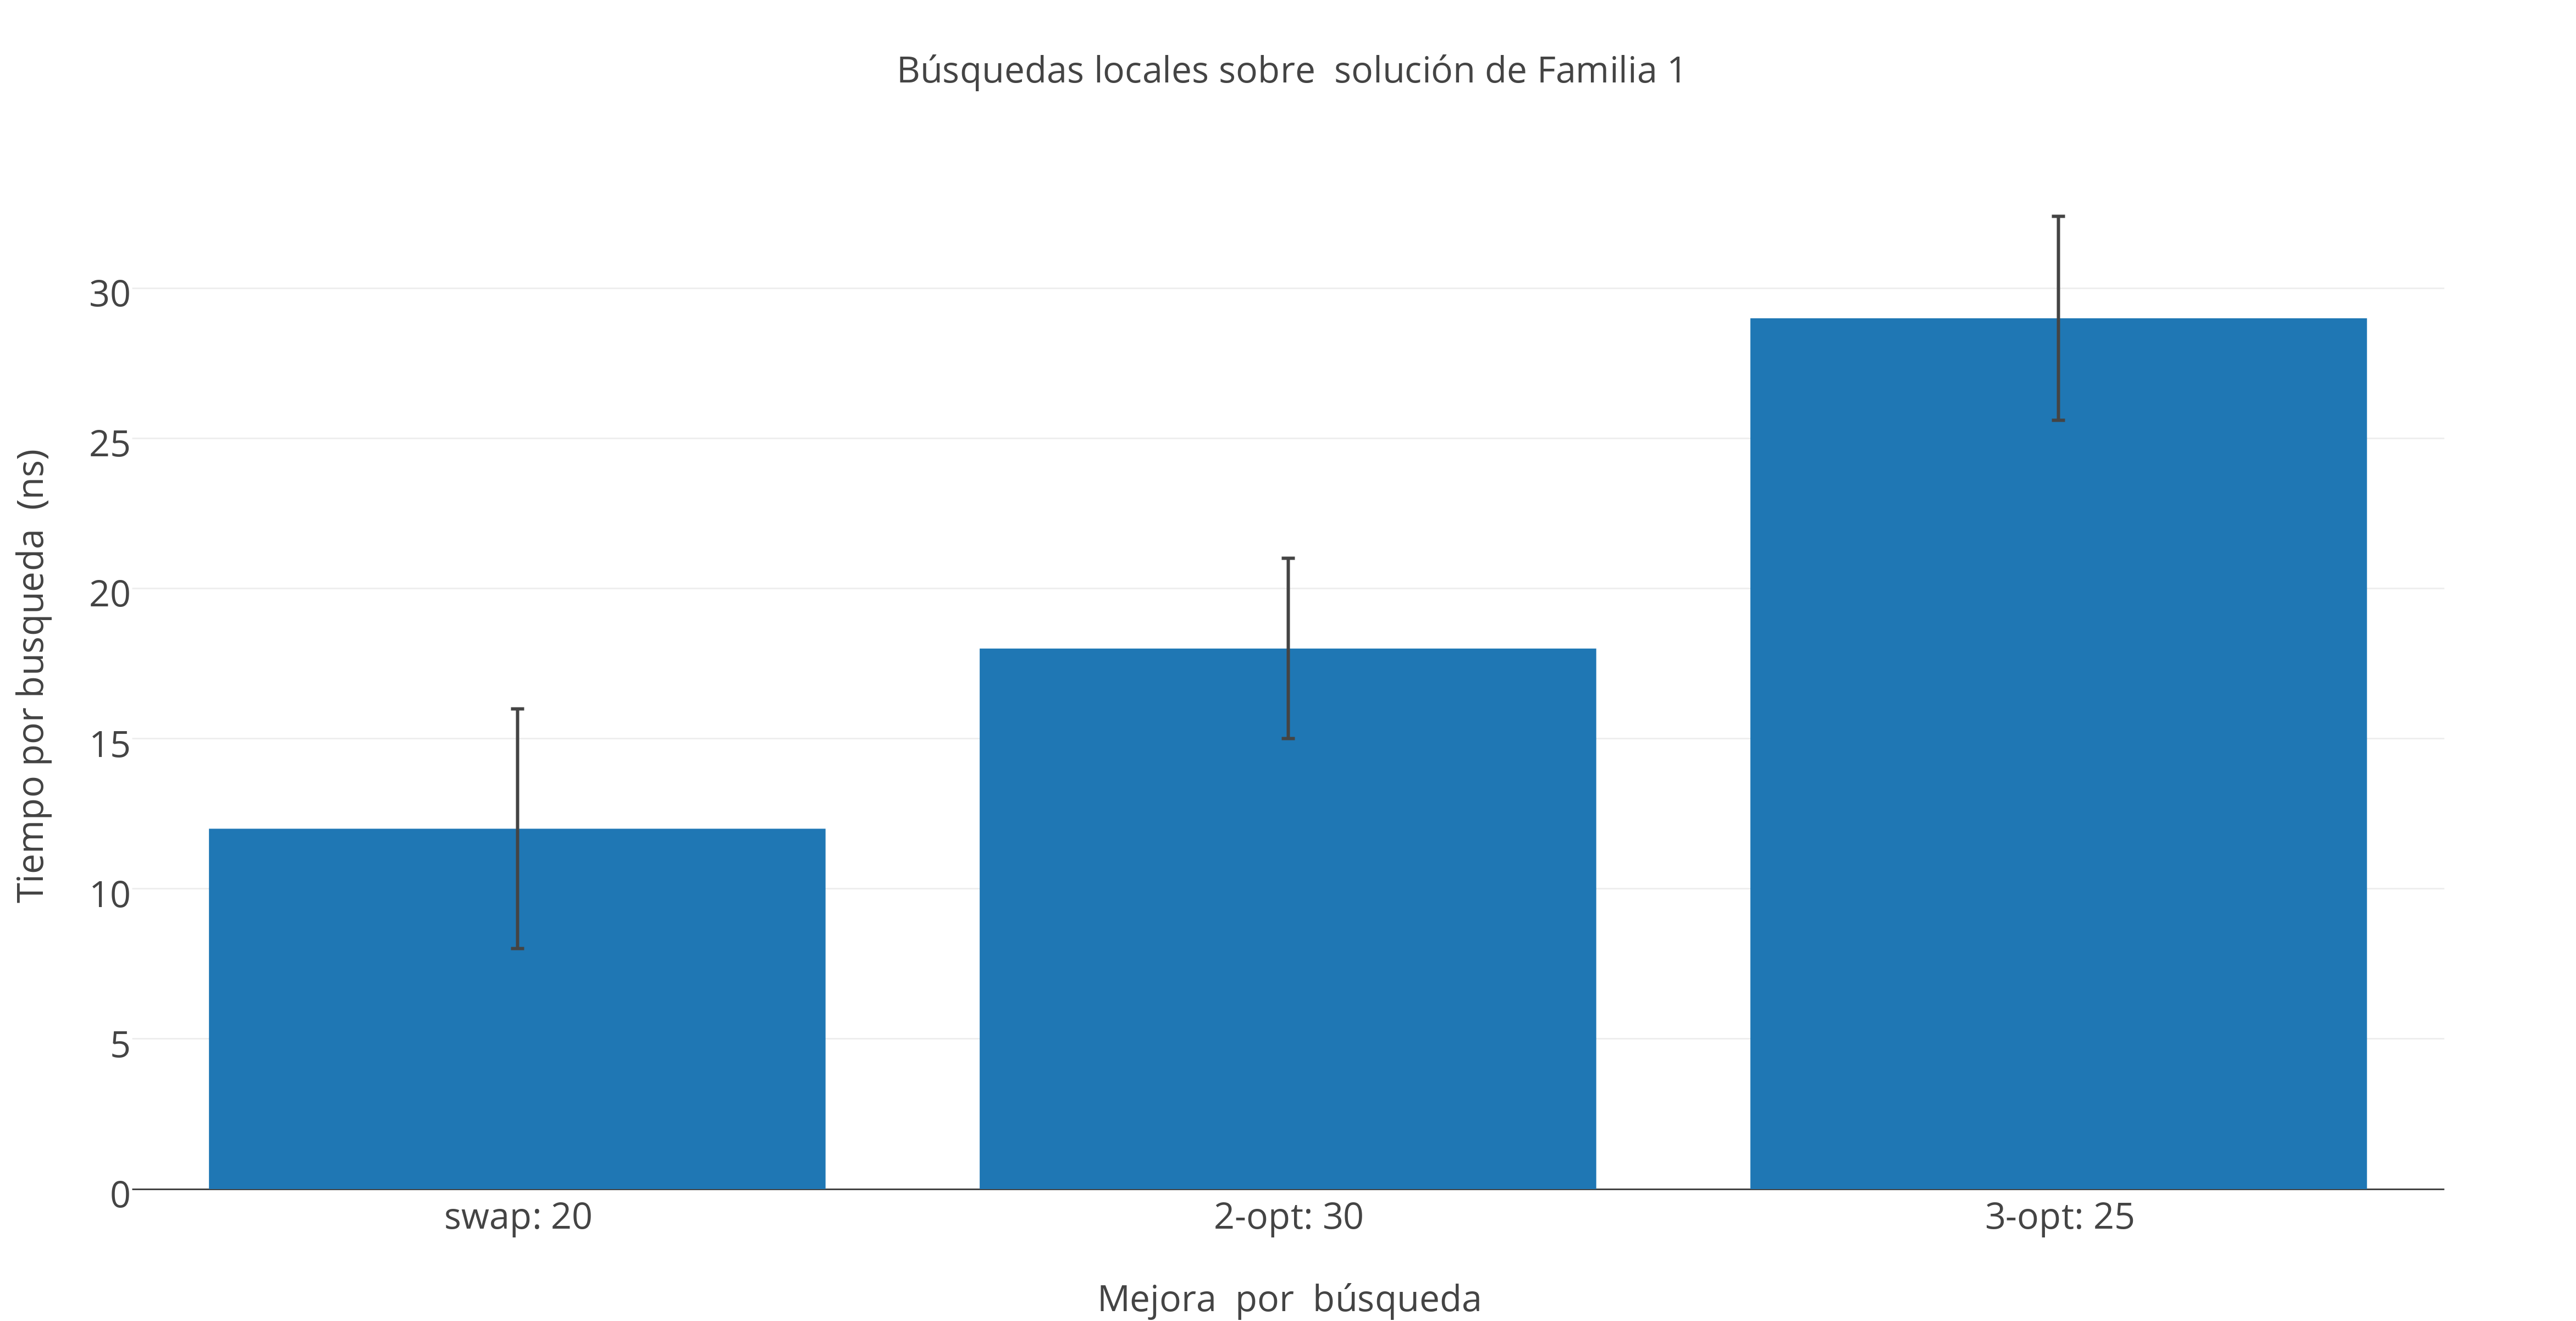
\includegraphics[scale=0.5]{./EJ3/local_search_familia.png}
 {            \textit{Gráfico \ 3.1 - Búsquedas locales sobre Familia 1}}
  \end{center}
  \vspace*{0.3cm}

\subsubsection*{Familia 2}

\vspace*{0.3cm} \vspace*{0.3cm}
  \begin{center}
 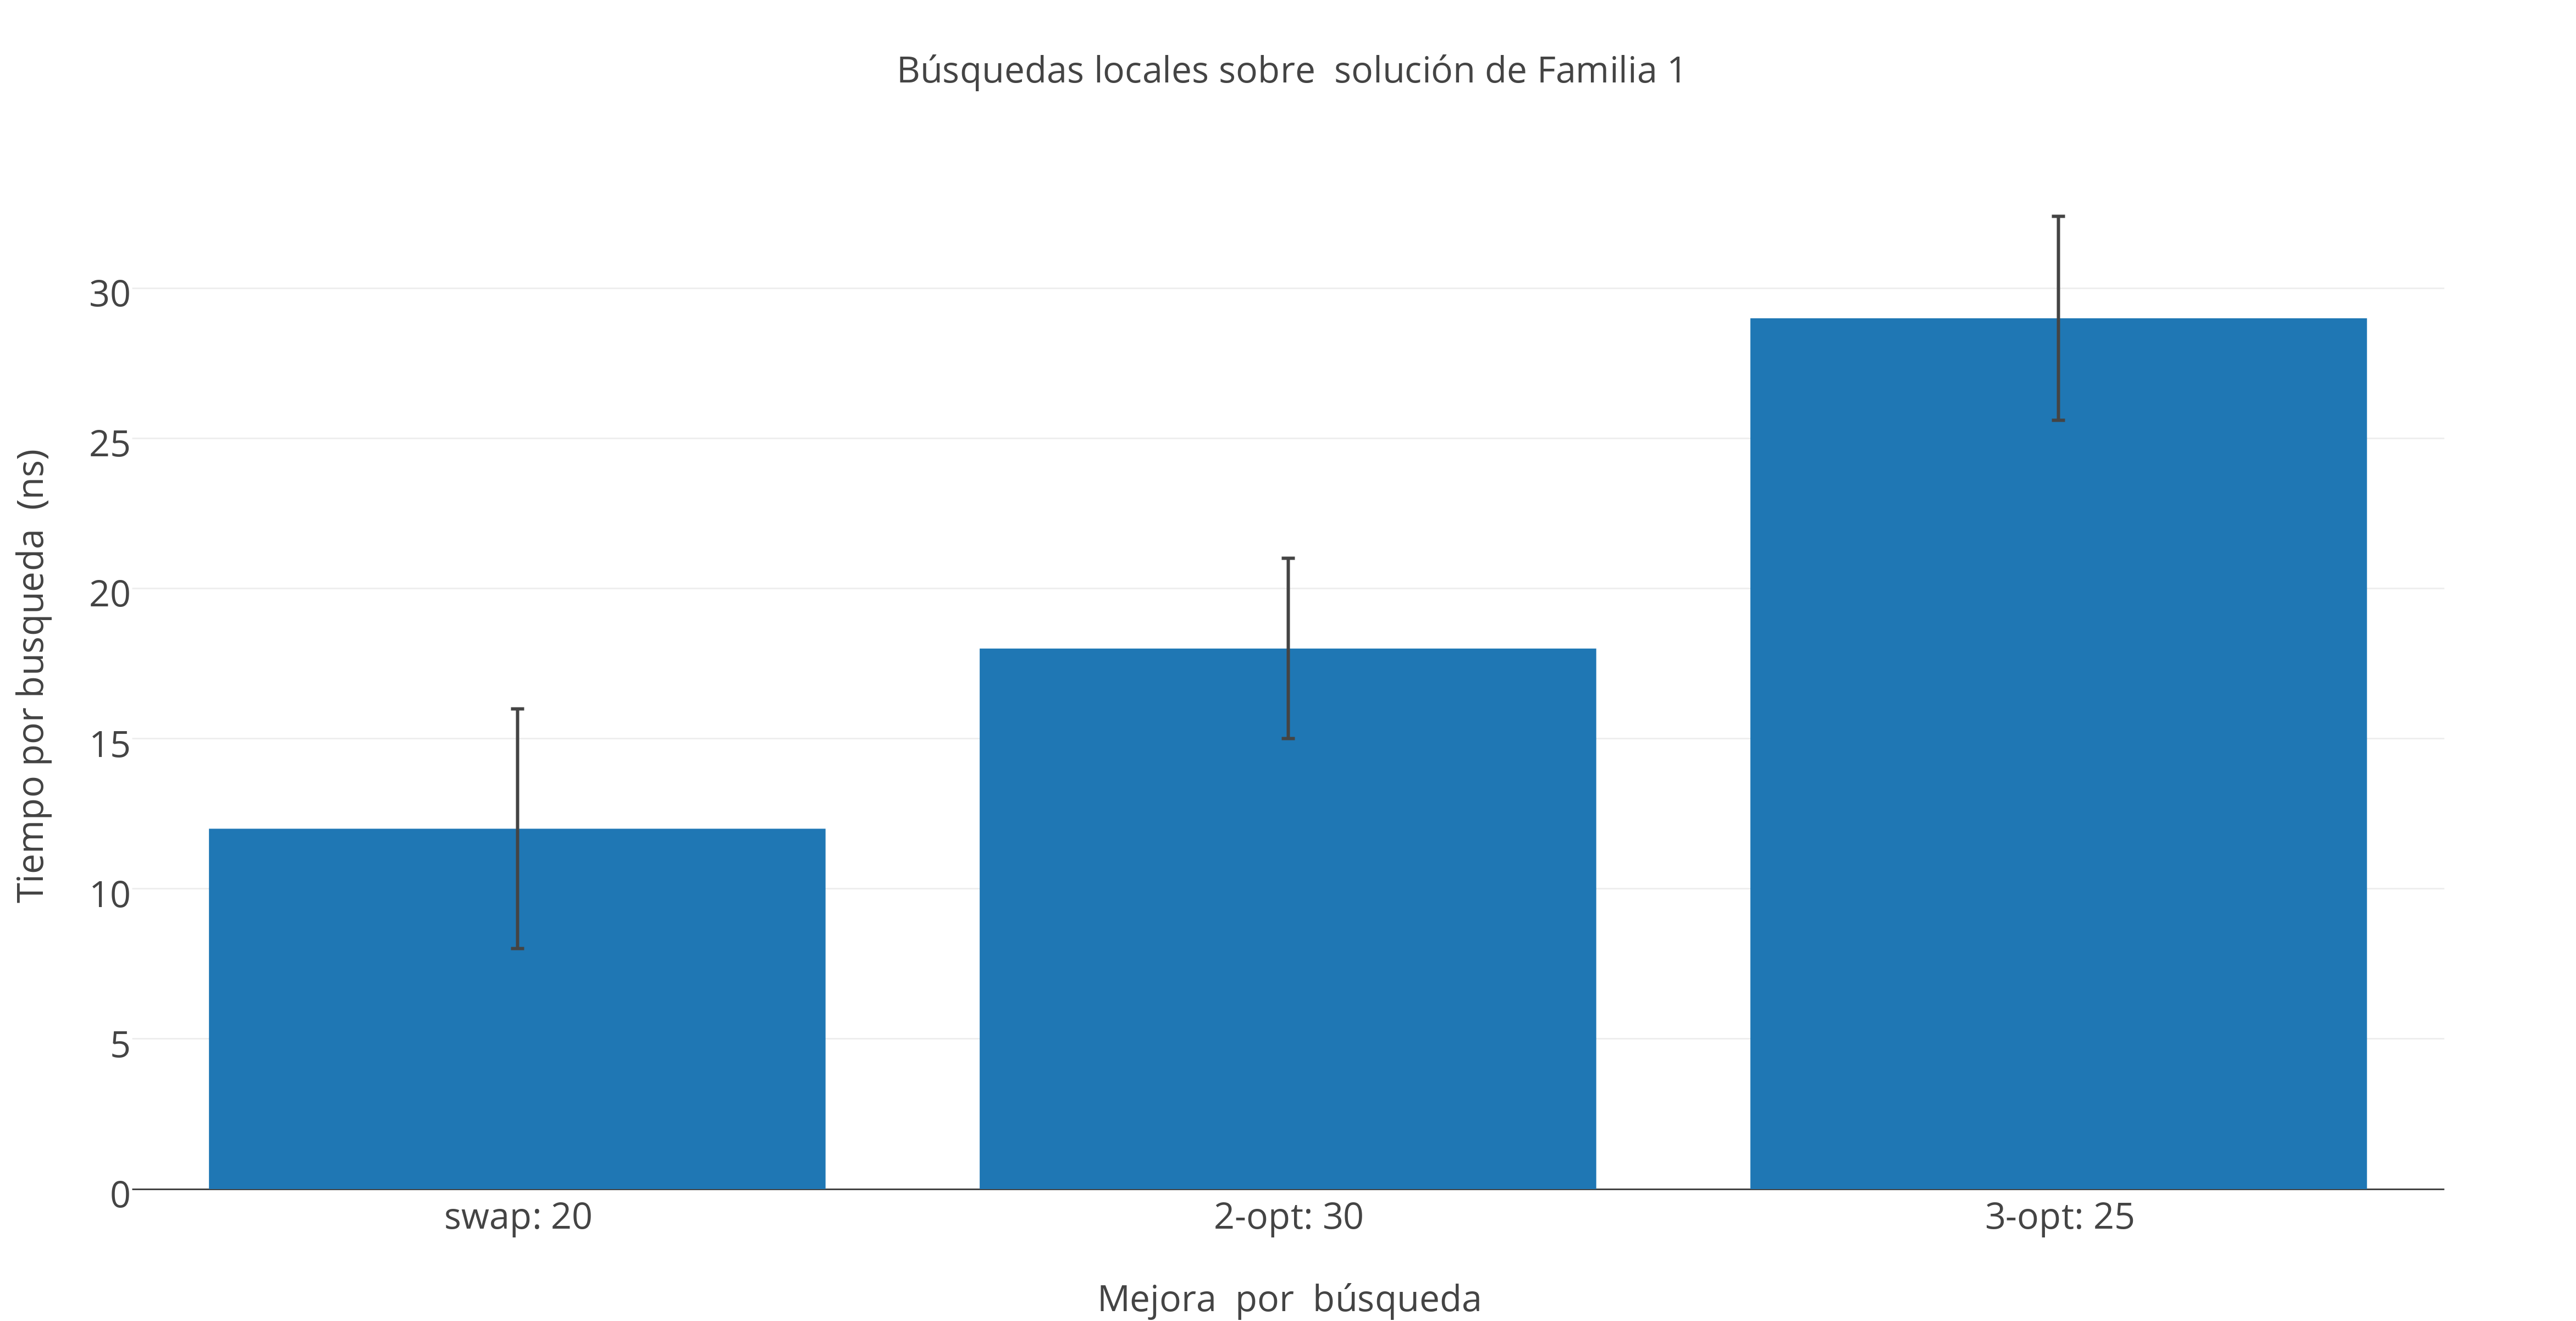
\includegraphics[scale=0.5]{./EJ3/local_search_familia.png}
 {            \textit{Gráfico \ 3.2 - Búsquedas locales sobre Familia 2}}
  \end{center}
  \vspace*{0.3cm}

\subsubsection*{Familia 3}

\vspace*{0.3cm} \vspace*{0.3cm}
  \begin{center}
 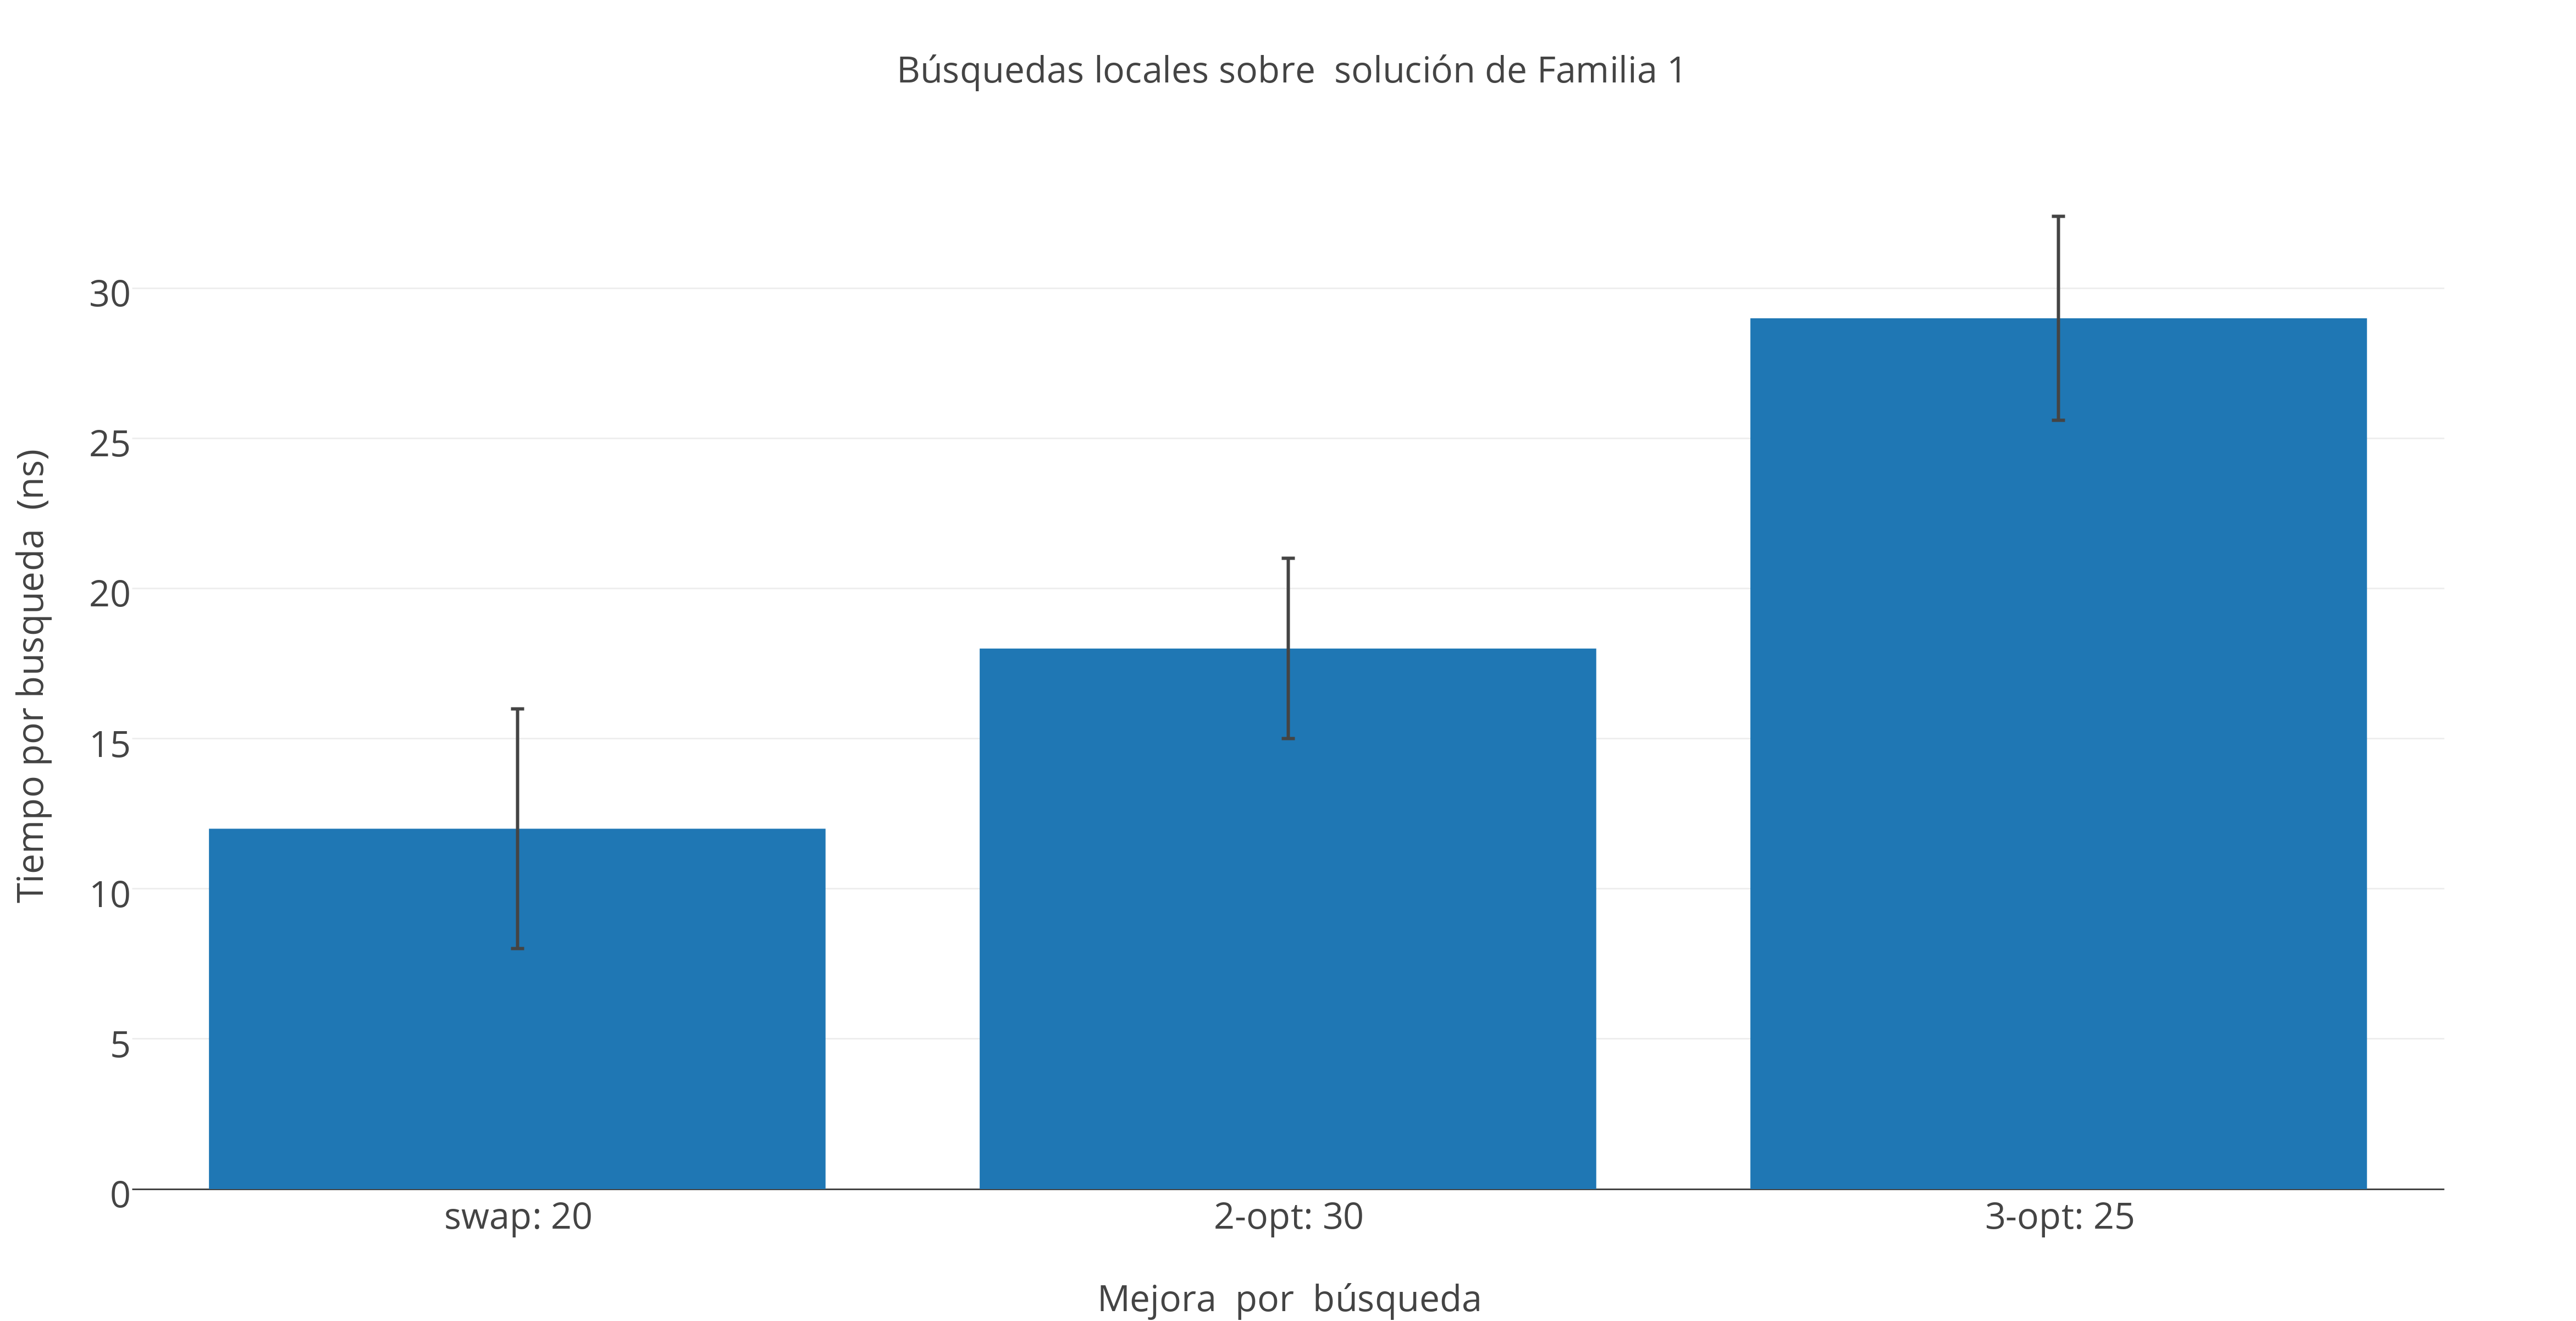
\includegraphics[scale=0.5]{./EJ3/local_search_familia.png}
 {            \textit{Gráfico \ 3.3 - Búsquedas locales sobre Familia 3}}
  \end{center}
  \vspace*{0.3cm}

\subsubsection*{Familia 4}

\vspace*{0.3cm} \vspace*{0.3cm}
  \begin{center}
 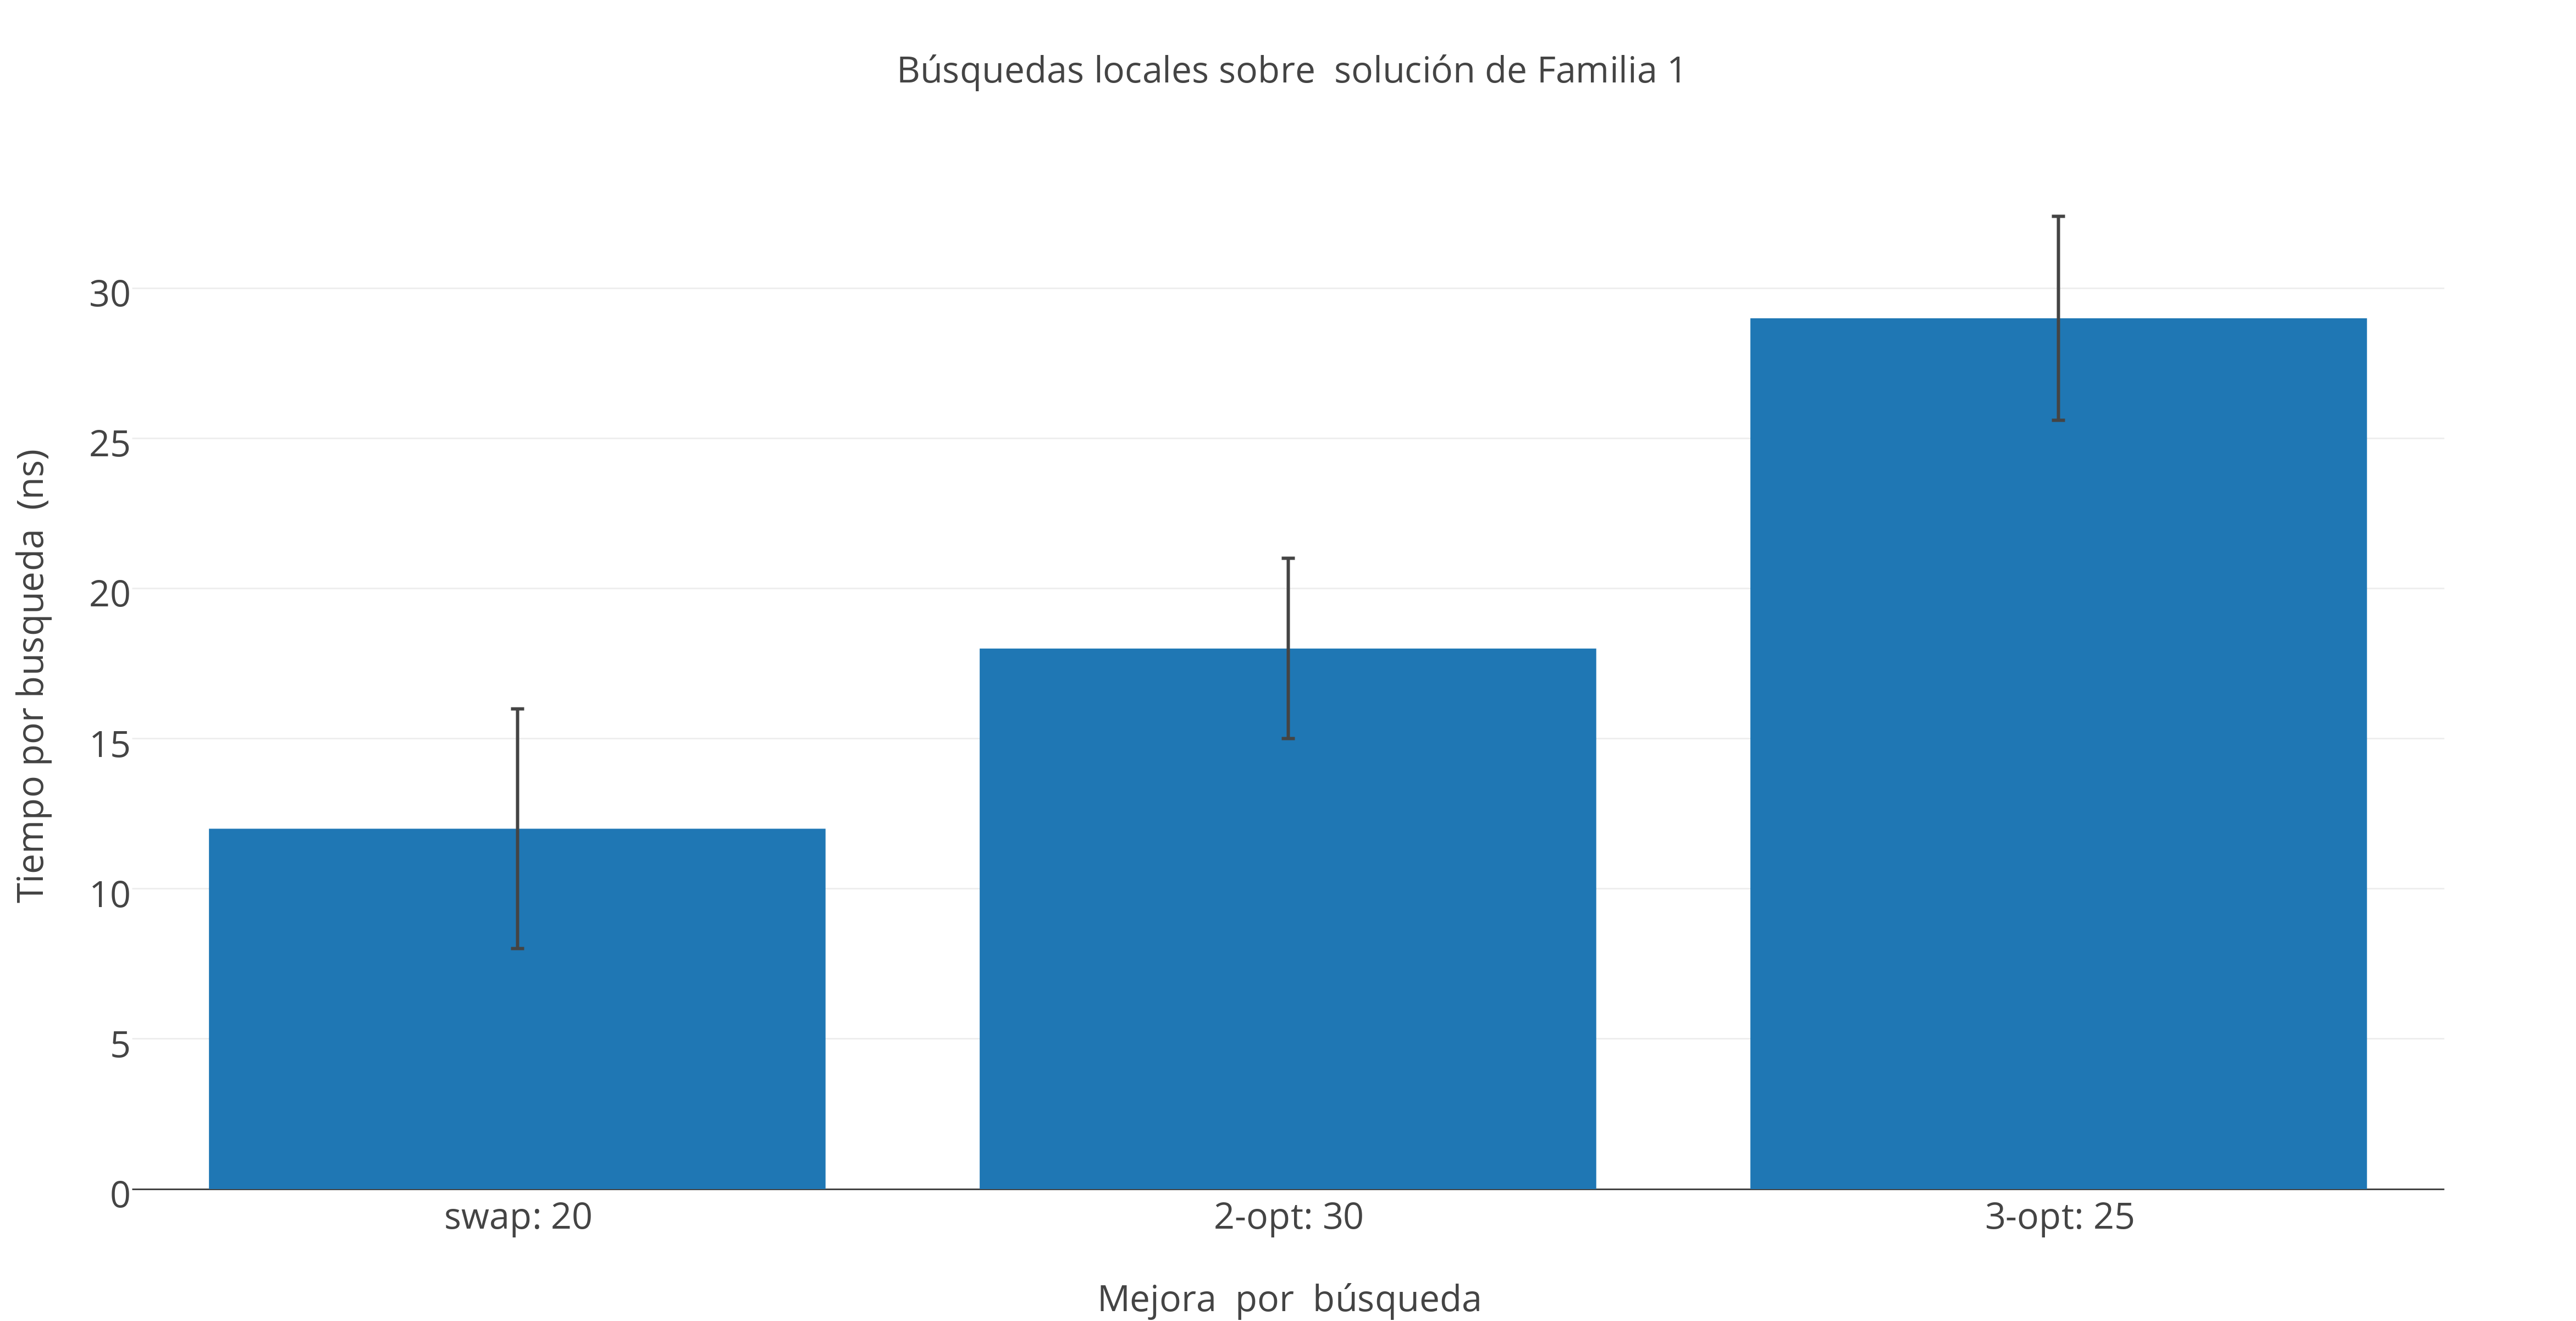
\includegraphics[scale=0.5]{./EJ3/local_search_familia.png}
 {            \textit{Gráfico \ 3.4 - Búsquedas locales sobre Familia 4}}
  \end{center}
  \vspace*{0.3cm}

%\subsubsection[2.5]{Performance de los algorítmos}
%\indent En esta secci\'on, mostraremos buenos y malos casos para nuestro algoritmo, y a su vez, daremos el tiempo estimado 
seg\'un la complejidad del algoritmo calculada anteriormente.

Para el mejor caso (aqu\'el en el que ninguna chica es amiga de otra), el gr\'afico obtenido es el siguiente:

\vspace*{0.3cm} \vspace*{0.3cm}
  \begin{center}
% 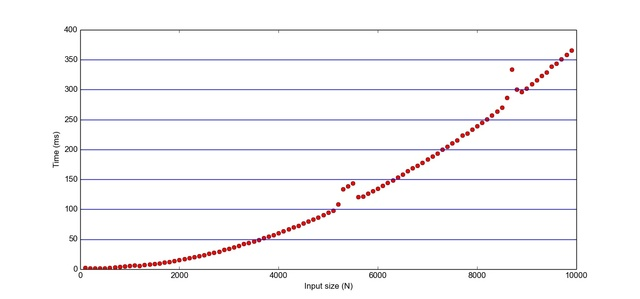
\includegraphics[scale=0.8]{./EJ3/resized2.jpg}
  \end{center}
  \vspace*{0.3cm}



\newpage
\section{Ejercicio 4} 
\subsection{Explicaci\'on de resoluci\'on del problema}
Como su nombre lo indica, búsqueda local analiza una vecindad local a la solución inicial $S_o$. Por lo que generalmente, la mejora obtenida puede no ser global, si no, la mejor solución dentro de la vecindad analizada. 

Para salir de un óptimo local, existen meta heurisiticas que pueden o no proveer una mejor solución observando otras vecindades, y en algunos casos acercarse lo suficiente u obtener el óptimo global. Una de ellas es la elegida para este informe, denominada, \textit{tab\'u search}.\\

La idea de esta meta heuristica es ir moviendose por las vecindades subyacentes a una vecindad analizada. Es decir, las vecindades de las soluciones que conforman una vecindad.
Pero no todas ellas, si no, la vecindad de una solución elegida que cumpla con ciertos atributos, o mejor dicho, que no posea ciertos atributos o caracteristicas. 
Esto es así, dado que se tiene que buscar una manera de descartar soluciones que no se consideren adecuadas para ser analizadas, si no, caeriamos en el problema de backtracking, donde se consideran todas las posibilidades, lo cual, puede ser impracticable.\\

Los atributos elegidos como no adecuados para elegir una solución son los denominados atributos \textit{tab\'u}. Existen muchas posibilidades según el problema estudiado. Para el problema del maestro pokemon eligiremos como atributos \textit{tabú} las aristas que sean modificadas al moverse de una solución a otra. Luego intentaremos ver que sucede al tomar como \textit{tabú} las aristas nuevas en la solución y ver si se obtienen mejores resultados.
Por lo tanto, se define un conjunto que alojará atributos \textit{tabú}.\\

Los métodos para encontrar vecindades serán los mismos analizados en el ejercicio tres. Es decir, a traves de las búsquedas locales estudiadas: $swap$, $2-opt$ y $3-opt$. Solo que para este algoritmo se filtrarán aquellos recorridos que no sean válidos. Luego una vecindad $V(s)$ para una solución $s$, será un conjunto de recorridos de soluciones válidas para el problema.\\

Debido a que la memoria tiene un limite, y los problemas podrian ser extremadamente grandes, se suele definir lo que se denomina \textit{tenor tabú} que es el tamaño máximo que el conjunto \textit{tabú} tiene para alojar atributos. Cuando el tamaño máximo es alcanzado, se tiene que determinar una manera de desalojar atributos para obtener espacio libre que pueda ser usado luego. El mótivo es tener una lista de tamaño acotado, pero que sea dinámica en contenido de atributos a lo largo de una corrida del algoritmo, dado que si no, al alcanzarse el tamaño máximo, la lista dejaria de crecer y los atributos dejarían de cambiar, acotando el universo de posibles soluciónes a la union de algunas vecindades.\\
Los atributos que serán desalojados serán aquellos que tengan más tiempo dentro del conjunto, por lo que además, el conjunto \textit{tabú} tendrá la caracteristica de poder contener esa información y funcionar internamente como pila. 
La cantidad de atributos desalojados será determinada por la cantidad de atributos que se quiera alojar en el conjunto. En el peor caso, todos los atributos serán nuevos.\\

Además, si el tenor definido en el punto anterior es lo suficientemente grande, indefectiblemente, en algún punto tendremos todos los atributos alojados. Por lo cual tendremos que tomar alguna decision para elegir una nueva solución en la vecindad analizada. Esta decision se conoce como función de aspiración $A(V(s)): \rightarrow s^{'}$ que dada una vecindad $V(s)$ a una solución $s$, determina que solución tomar.
La decision puede tomarse en base a la cantidad de atributos \textit{tabú} que posee la solución analizada. Luego puede elegirse la más tabú o la menos tabú.
En este informe estudiarmos ambas metodologias y veremos cual nos ofrece mejores resultados.\\




 
 
\subsection{Pseudoc\'odigo}
Como comentario inicial, se presenta el algoritmo $Tabu$ $Search$ con ambos criterios de parada en el ciclo principal (cantidad de iteraciones límite y cantidad de iteraciones sin mejora) ya que ambos pueden aplicarse a la vez o por separado que es como serán estudiados en la experimentación.

El algoritmo itera sobre una solución inicial $S_o$ que es un vector con los $id$'s de las pokeparadas y gimnasios como fue definido en el ejericio tres. \ref{sec:alg3} 
Se utiliza el vector $solucionActual$ para guardar el recorrido que se utiliza para recorrer vecindades. Mientras que $mejorSolucion$ guarda el mejor recorrido encontrado en todas las vecindades analizadas y será este el encargado de hacer valer la condición de corte de cantidad de iteraciones sin mejora.

El algoritmo procede a calcular la vecindad de $solucionActual$ filtrando aquellos recorridos no válidos para el problema en cuestión (las condiciones de validez de una solución fueron dadas en el ejercicio dos) y luego busca el mejor candidato dentro de esta vecindad, que será aquella con menor costo y que no sea un recorrido marcado como tabú (es decir que previamente ya fue tomado).

Si no obtuvo un candidato, procede a utilizar la función de aspiración, que será elegir aquel recorrido en el vecindario que sea menos tabú.

En cualquier caso, siempre se obtienen las aristas modificadas para llegar a este recorrido dentro de la vecindad (esto depende de la búsqueda local utilizada) y se agregan las mismas a la lista tabú.

Una vez hecho esto se actualiza el $mejorCosto$ y la $mejorSolucion$ si el recorrido encontrado mejora el $mejorCosto$ actual. Si esto no sucede, se aumenta en una unidad la cantidad de iteraciones sin mejora. 

El algoritmo finaliza cuando se alcanza la cantidad de iteraciones límite o la cantidad de iteraciones sin mejora límite. Una u otra dependen de la elección del usuario.

\begin{algorithm}[H] %or another one check
 \Fn{tabuSearch()}{
 %     \SetAlgoLined
 $S_o$ es la solución provista por el algoritmo greedy \\
 ConjuntoTabu attributosTabu \hfill O(n) \\ 
 Recorrido mejorSolucion $\leftarrow$ $S_o$ \hfill O($n$)\\
 Recorrido  solucionActual $\leftarrow$ $S_o$ \hfill O($n$)\\ 
 entero mejorCosto $\leftarrow$ calcularCosto(mejorSolucion) \hfill O($n$)\\
entero iter = 0\\
entero MaxIter = cantidad pokeparadas+cantidad gimnasios \\
entero TenorTabu = MaxIter \\ 
entero MaxNoMejora = 4 \\ 

 \For{iter < MaxIter $\wedge$ entero noMejora < maxNoMejora }{
	 \hfill ciclo: O($Critero Parada$)\\
	Recorrido mejorCandidato \hfill O(1) \\
  	Lista<Arista> aristasModificadas \hfill O(1)\\
  	entero costoMejorCandidato $\leftarrow$ -1 \hfill O(1)\\
  	
	Conjunto<Recorrido, Lista<Arista> > vecindadActual $\leftarrow$ vecindadFiltrada(solucionActual) \hfill O($n^4$)\\
  	
  	\For{par en vecindadActual}{
		\hfill Ciclo: O($n^4$)\\
  		Recorrido candidatoActual $\leftarrow$ par.first \hfill O(n)\\
  		entero costoActual $\leftarrow$ calcularCosto(candidatoActual) \hfill O($n$)\\
		costoMejorCandidato  	$\leftarrow$ calcularCosto(mejorCandidatol) \hfill O($n$)\\
		
		\If{costoActual < costoMejor $\vee$ (!tabuCount(atributosTabu, candidatoActual) $\wedge$ (costoActual < costoMejorCandidato $\vee$ costoMejorVecino = -1)}{
			\hfill Condicion: O($n$)\\
			aristasModificadas $\leftarrow$ par.second \hfill O(1) \\%|par.second|<=4
			mejorCandidato $\leftarrow$ candidatoActual \hfill O($n$)\\
		}
  	}  	
	\hfill Total del ciclo: O($n^5$)

	\If{no se encontro mejorCandidato}{
		\hfill Condicion: O(1)\\
		<Recorrido, Lista<Arista> > menosTabu $\leftarrow$ funcionAspiracion(atributosTabu, vecindadActual) 
		\hfill O($n^5*log(TenorTabu)$)\\%
		
		mejorCandidato $\leftarrow$ menosTabu.first \hfill O($n$)\\
		aristasModificadas $\leftarrow$ menosTabu.second \hfill O(1)\\
	}  	
	
	costoMejorCandidato = calcularCosto(mejorCandidato); \hfill O($n$) \\
	
	solucionActual $\leftarrow$ mejorCandidato \hfill O($n$)\\
		
	\If{costoMejorCandidato $<$ mejorCosto}{
		\hfill Condicion: O(1)\\
		mejorSolucion $\leftarrow$ mejorCandidato \hfill O($n$)\\
		mejorCosto $\leftarrow$ costoMejorCandidato \hfill O(1)\\
		noMejora=0\\
	}\Else{
		noMejora+=1\\
	}
		iter+=1 \\
}
agregarAtributosTabu(AristasModificadas)\\
devolver mejorSolucion \\
}

\end{algorithm}
	
\begin{algorithm}[H]

\Fn{agregarAtributosTabu(aristasModificadas)}{
%     \SetAlgoLined
   \For{Arista a en aristasModificadas}{
	 	\hfill Ciclo: O(1)\\
	   atributosTabu.push(a) \hfill O(l$log(TenorTabu)$)\\
   }
  	
   \While{|atributosTabu| > TenorTabu}{
	   \hfill Ciclo: O(1)\\
	   atributosTabu.pop() \hfill O($log(TenorTabu)$)\\
   }
}


\end{algorithm}

Complejidad final: 
 O($CriterioParada$ * ( $n^5$ $\ast$ $log(TenorTabu)$ + $TenorTabu$)) =  O($CriterioParada$ * ( $(N+M)^5$ $\ast$ $log(TenorTabu)$ + $TenorTabu$)) \\
Siendo $N$ = cantidad pokeparadas y $M$ = cantidad gimnasios.\\

En general a la hora de implementar y experimentar, serán tomados porcentajes de $N+M$ para la cantidad de iteraciones límite y el tenor tabú ya que pueden ser valores muy grandes.\\

\subsubsection*{Detalles del algoritmo}

\begin{itemize}
Justificación de la cota de complejidad del ciclo principal:
\item $CriterioParada$: Este parametro determina cuantas veces ejecuta el ciclo principal de la busqurda tabu. Toma el minimo entre el valor $MaxIter$ y ($maxNoMejora$ - 1) * costoInicial.
\item Este ultimo valor es cota superior de la cantidad de iteraciobnes ya que en peor caso pueden pasar ($maxNoMejora - 1$) iteraciones sin que se mejore la solucion. Y esta mejora es, en peor caso 1. Como el costo es mayor a cero, se itera como mucho ($maxNoMejora$ - 1) * $costoInicial$ veces.
\item Luego, el algoritmo finaliza si se producen $maxNoMejora$ cantidad de iteraciones sin mejora de $costoInicial$ o si se alcanza $MaxIter$. 
\item En el peor caso $n = N+M$ es decir, que la solución inicial del algoritmo tiene todas las pokeparadas y gimnasios del mapa.
\item Arista = < Punto a , Punto b >
\item Punto = < entero x, entero y >
\item La función $calcularCosto$ ya fue definida en el apartado del algoritmo del ejercicio 3.
\item La función $vecindadFiltrada$ devuelve una lista de tuplas. Cada tupla posee una de las soluciones vecinas (obtenida a partir de algún movimiento: 2opt, 3opt o swap) y las aristas que se modificaron para llegar a esa solución. La soluciones han sido previamente "filtradas"; es decir, una solucion solo puede estar en esta lista si es una solución válida para nuestro problema. Generar vecindades 2opt y swap tiene complejidad O($n^3$), en cambio las vecindades 3opt toman O($n^4$).
	La cantidad de soluciones de cada vecindad está acotada de la misma manera que sus complejidades. En peor caso, se encontró una solucion válida en cada iteraci\'on.
\item La función $funcionAspiracion$ devuelve dada una vecindad y los atributos tabú, el recorrido que menos atributos tabú tenga y además las aristas modificadas para obtener ese recorrido. Implica iterar sobre la vecindad y sobre los atributos tabú. 
\item La funcion $tabuCount$ sirve para decidir si una solución es tabú o no y cuenta cuantos atributos tabú posee dando de esta manera una medida de "cuan tabú" es una solución. Se itera por las aristas de la solución en tiempo lineal.
\item $atributosTabu$ está implementado sobre el set proveido por la STL de c++. Se observa una estructura de arbol rojinegro que puede buscar, insertar y borrar en un tiempo O($log(TenorTabu)$), y se mantiene la cantidad de elementos de este por debajo de $TenorTabu$.
\end{itemize}

\subsection{An\'alisis de complejidades}
Con la idea utilizada en la demostración de finalización de nuestro algoritmo podemos generar una cota para la complejidad de los algoritmos planteados en esta sección. \\
Si en nuestro algoritmo realizamos $K$ pasadas, quiere decir que mejoramos la solución en $K - 1$ pasadas, es decir, aumentamos la cantidad de aristas buenas en $K - 1$ pasadas. Como la cantidad de aristas buenas es como mínimo $0$ y como mucho $E$ y en cada pasada aumentamos en al menos $1$ la cantidad de aristas buenas, realizamos como mucho $O(E)$ pasadas. \\
Como en cada pasada, iteramos los $V$ nodos, esto nos da que la complejidad de los algoritmos es $O(E * V * X)$ donde $X$ es lo que cuesta procesar un nodo en particular para intentar mejorar la solución. \\

Para la primer vecindad, en el peor de los casos probamos con todos los colores. Probar con un color hace tantas operaciones como vecinos tenga un nodo, por lo que es $O(E)$, como lo hace para cada color, la complejidad termina siendo $O(E^2 * V * C)$, con  $C$ la cantidad total de colores. La complejidad de una iteración resulta $O(V * E * C)$\\

Para la segunda vecindad, calcular el mejor color y setearlo tiene costo $O(E)$ (hace tantas operaciones como vecinos tenga), por lo que la complejidad termina siendo $O(E^2 * V)$. La complejidad de una iteración resulta $O(V * E)$. \\

\subsection{Experimientos y conclusiones}
\subsubsection[2.5]{Test y performance del algorítmo}
Queremos observar que tan bueno es el algoritmo propuesto en la práctica. Para esto realizaremos una serie de tests utilizando las entradas que se utilizaron en el ejercicio 3.
La idea es tratar de encontrar la configuración ideal para que en promedio el algoritmo resuelva la mayoria de los casos eficientemente. Para lograr esto, experimentamos variando distintos parametros para cada entrada y obtener las respectivas conclusiones de los resultados obtenidos.\\
Los parámetros de estudio fueron:

\begin{enumerate}
\item  \textbf{Cantidad de iteraciones}: Tenemos que observar en promedio, cuantas iteraciones conviene tomar para obtener un buen resutado.
\item \textbf{Tenor tabú}: Tenemos que observar que sucede al aumentar el tenor tabú, y hasta cuanto es conveniente hacerlo para obtener un buen resultado.
\item \textbf{Atributos tabú}: Analizar que sucede al tomar como atributos tabú las aristas que cambiaron o las aristas nuevas
\item \textbf{Función de aspiración}: Elegir la solución más tabú o la menos tabú.
\end{enumerate}

Debemos aclarar, que tenor tabú fué establecido en cantidad de pokeparadas mas gimnasios. Este valor puede ser relativamente grande, pero cuanto más grande, más tiempo de resolución es necesario, con lo cual al final no es una cuestion de memoria, si no, una cuestion de tiempo de computos necesaria para correr el algoritmo.
También se trabajó probando diferentes configuraciones de atributos tabú y función de aspiración, obteniendo en todos los casos los mismos resultados, por lo que al final se decidió dejar prefijado el estandar para tabú search que es aristas viejas como atributos tabú y solución menos tabú para la función de aspiración.\\

Se tomaron 20 mediciones por cada tipo de test y se tomó una media alfa podada de las mismas con $\alpha$ = 0.5 de manera de podar un 25\% de los datos a cada lado.  De esta forma se reduce la posibilidad de outliers en las muestras consideradas.

Como fue enunciado en incisos anteriores de este trabajo las 4 familias en las que la heur\'istica golosa no otorga una soluci\'on \'optima son:

\begin{enumerate}
\item Familia 4
\item Familia 6
\item Familia 7
\item Familia 8
\end{enumerate}

Estas ser\'an las únicas a ser a analizadas, ya que el resto son el resultado exacto o no tienen soluci\'on, con lo cual no aportan mayor relevancia.
 
\subsubsection*{Familia 4}

Veamos algunos resultados de aplicar cada version de tabú search:

\vspace*{0.3cm} \vspace*{0.3cm}
  \begin{center}
 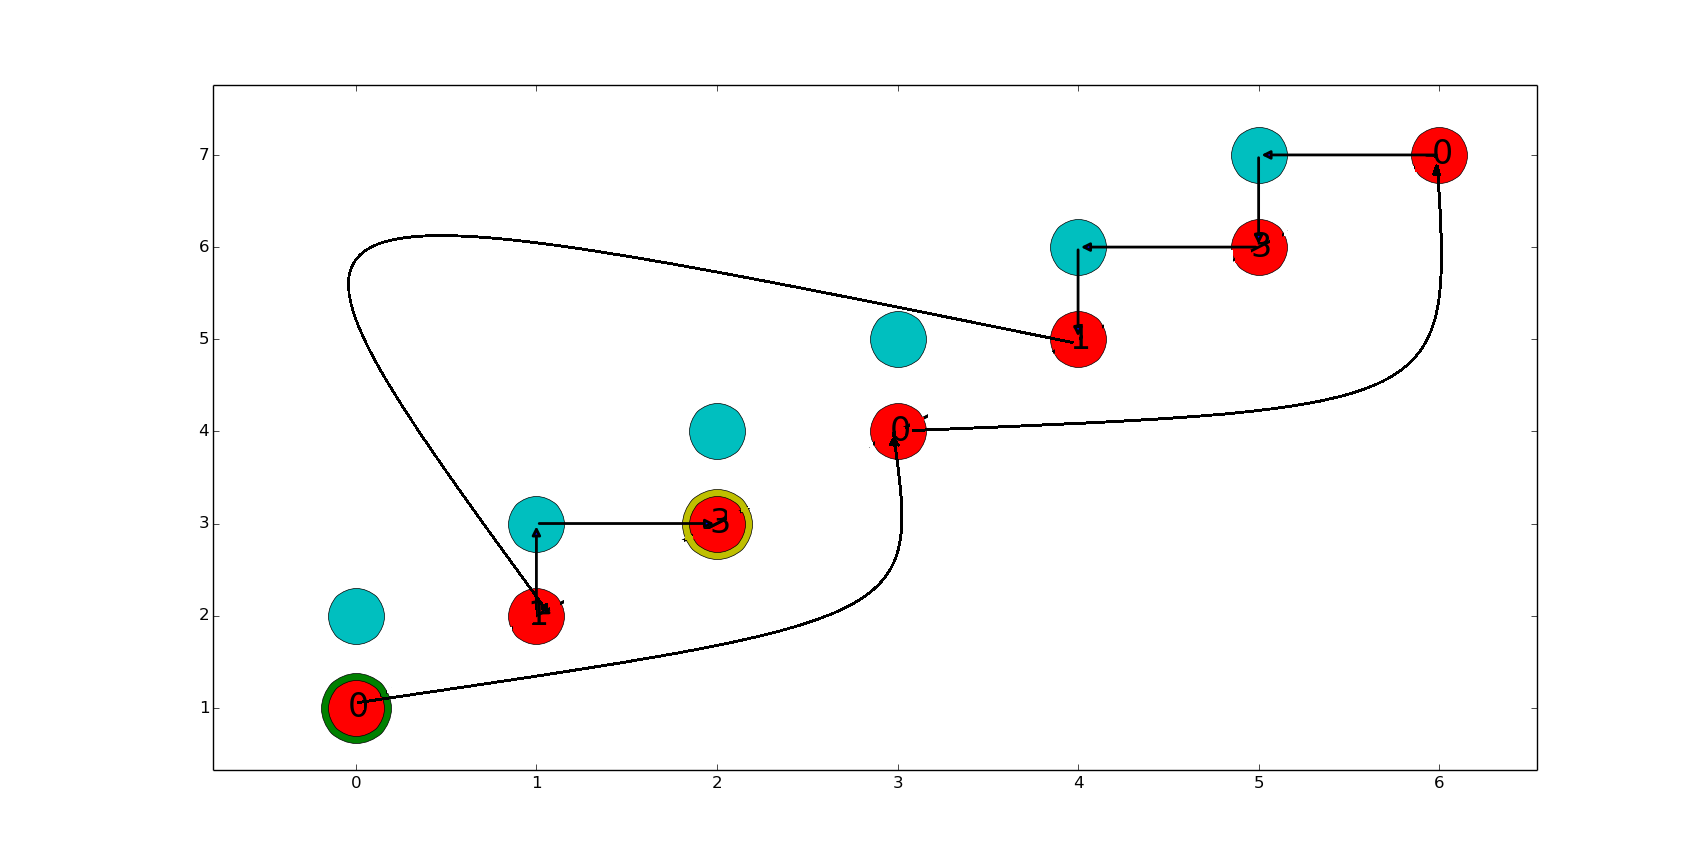
\includegraphics[scale=0.3]{./EJ4/fam4goloso.png}\\
 {            \textit{Soluci\'on Golosa}}
  \end{center}
  \vspace*{0.3cm}

\vspace*{0.3cm} \vspace*{0.3cm}
  \begin{center}
 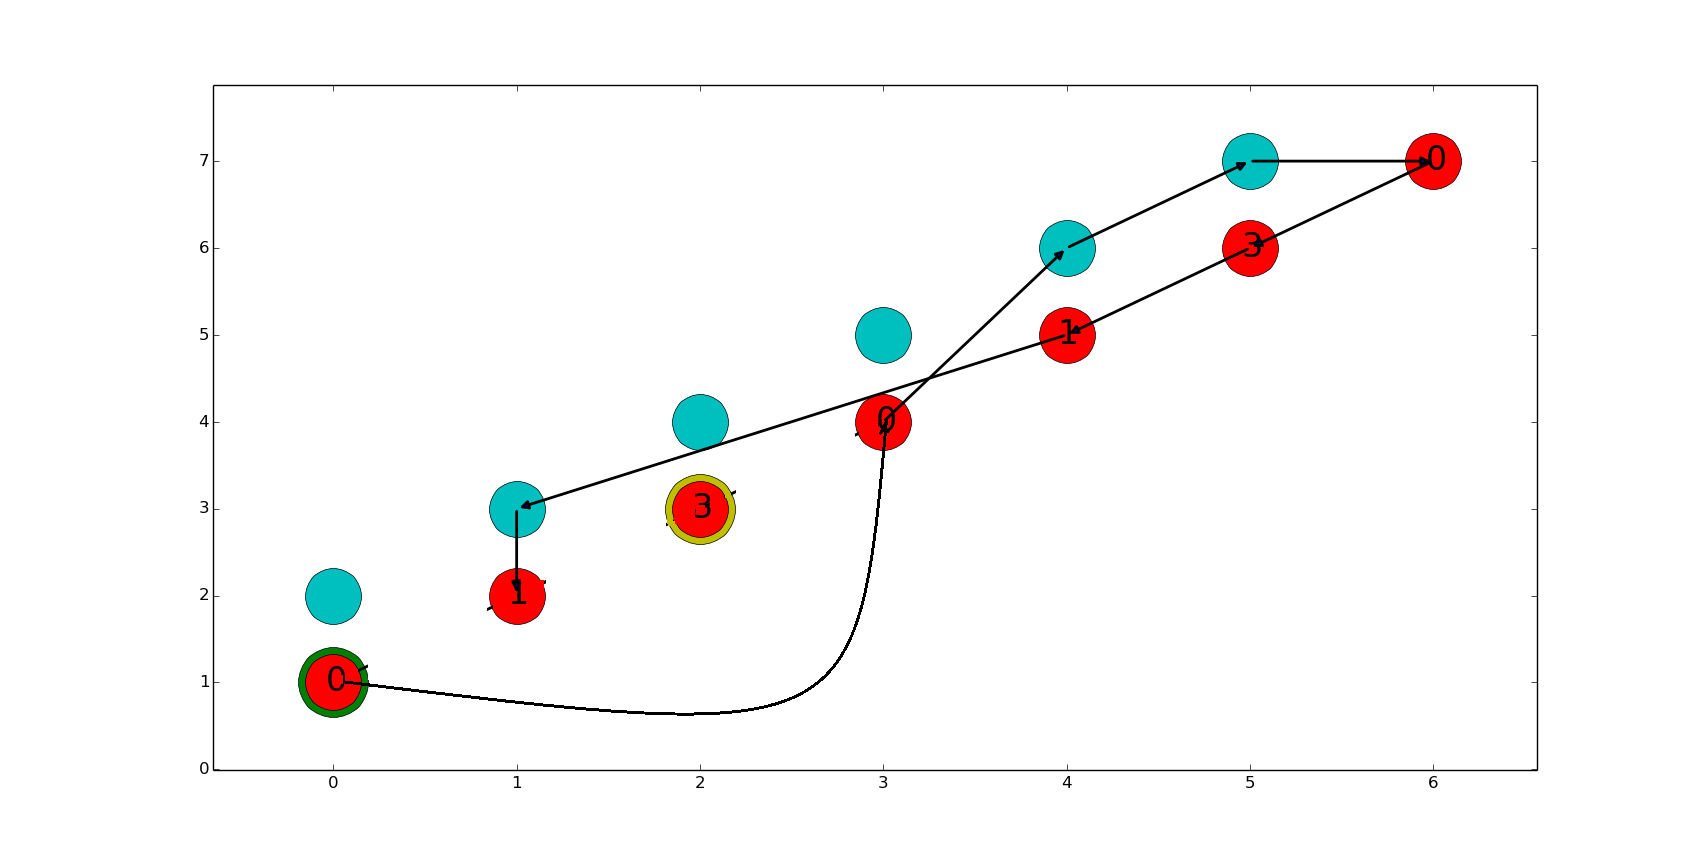
\includegraphics[scale=0.3]{./EJ4/fam42opt.png}\\
 {            \textit{Soluci\'on 2-OPT}}
  \end{center}
  \vspace*{0.3cm}

\vspace*{0.3cm} \vspace*{0.3cm}
  \begin{center}
 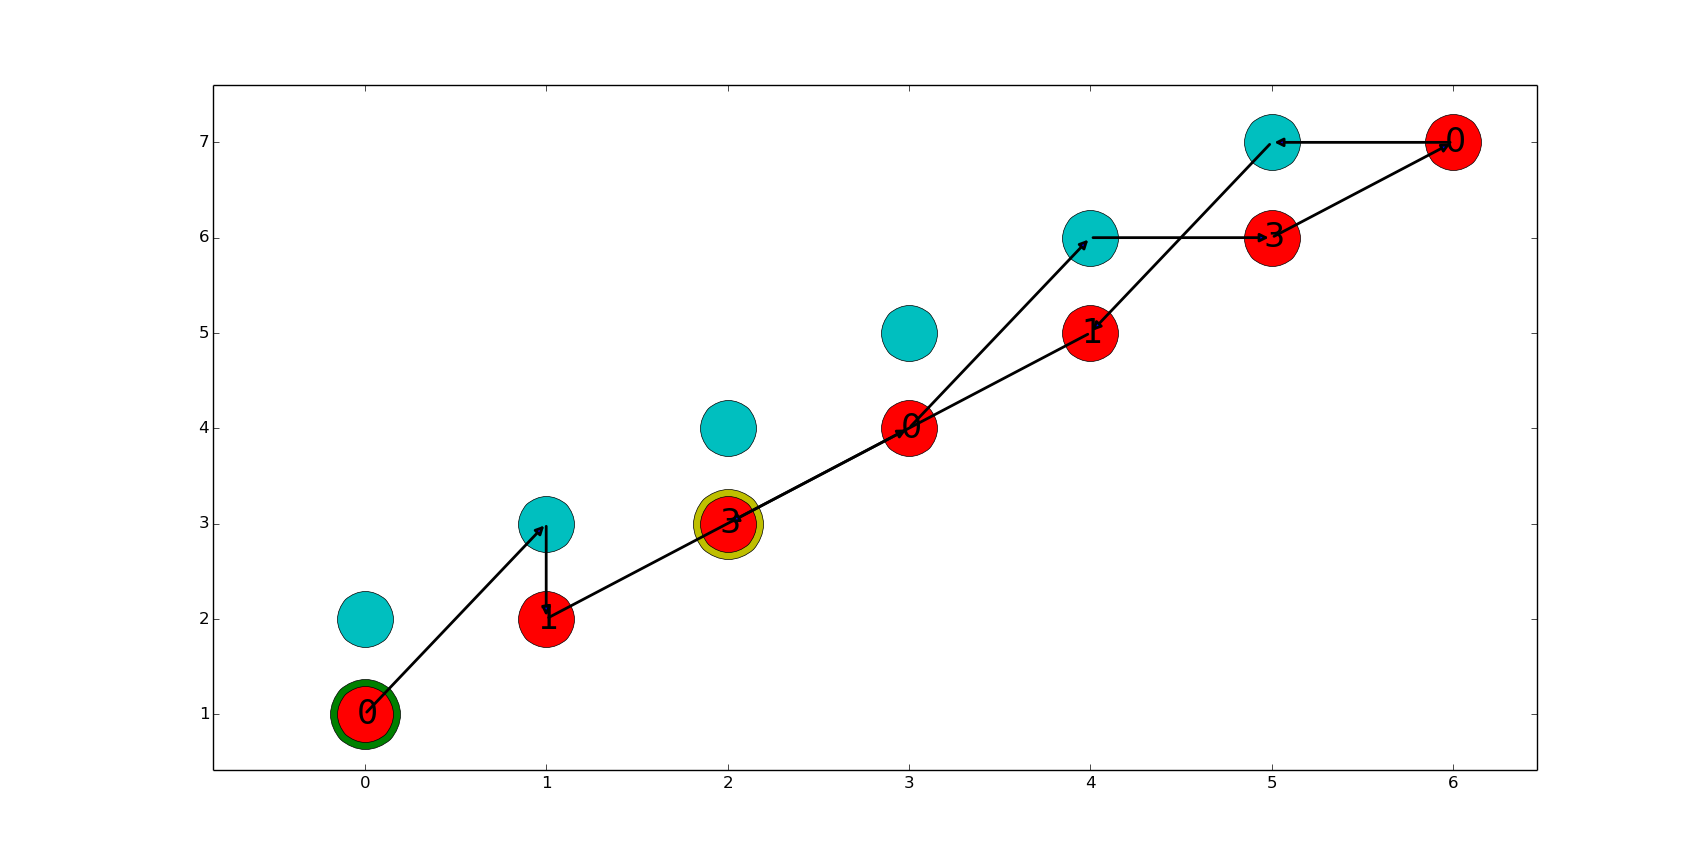
\includegraphics[scale=0.3]{./EJ4/fam43opt.png}\\
 {            \textit{Soluci\'on 3-OPT}}
  \end{center}
  \vspace*{0.3cm}

Nos parece interente comparar los resultados de mejora y tiempo de las búsquedas locales y tabú search que utilicen la misma vecindad, para ver si tabú search mejora lo logrado por la búsqueda local o empeora el resultado. Esto será realizado para cada familia mencionada.\\

Veamos como se comporta tabú 2-OPT con respecto a la heuristica de búsqueda local 2-OPT dentro de la familia 4:

\vspace*{0.3cm} \vspace*{0.3cm}
  \begin{center}
 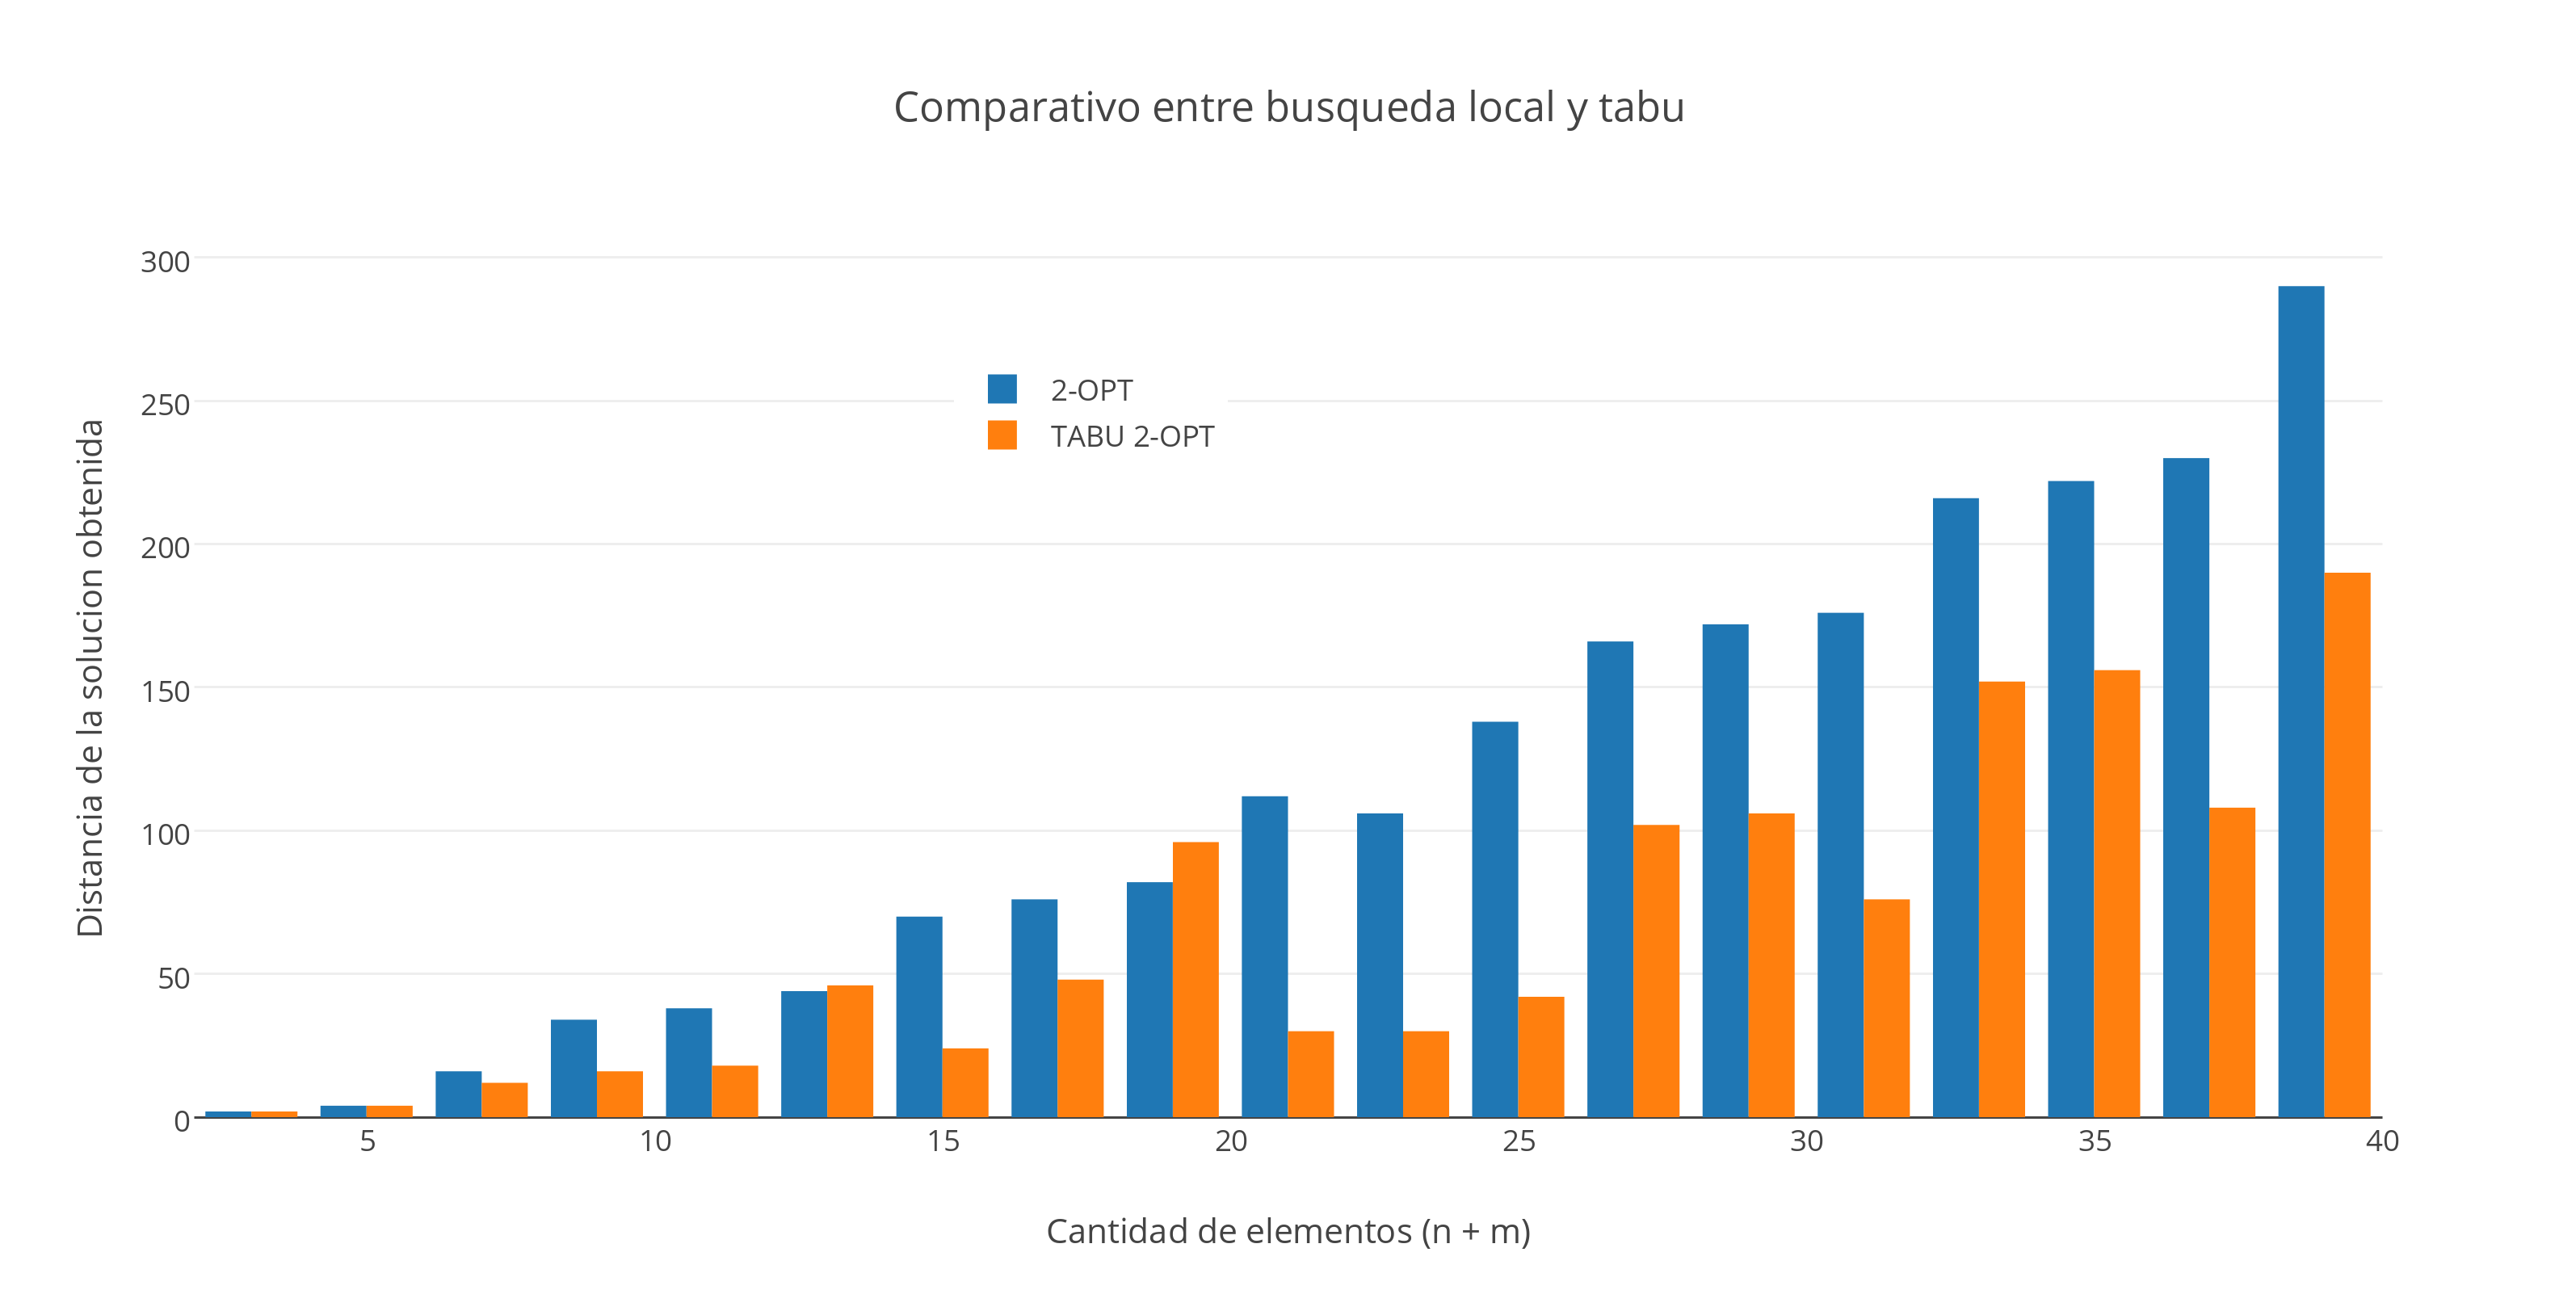
\includegraphics[scale=0.5]{./EJ4/comparativogym02opt.png}\\
 {            \textit{Gráfico \ 4.1 - 2-OPT vs Tabu 2-OPT sobre Familia 4}}
  \end{center}
  \vspace*{0.3cm}

En cuanto a tiempo insumido vemos lo siguiente:

\vspace*{0.3cm} \vspace*{0.3cm}
  \begin{center}
 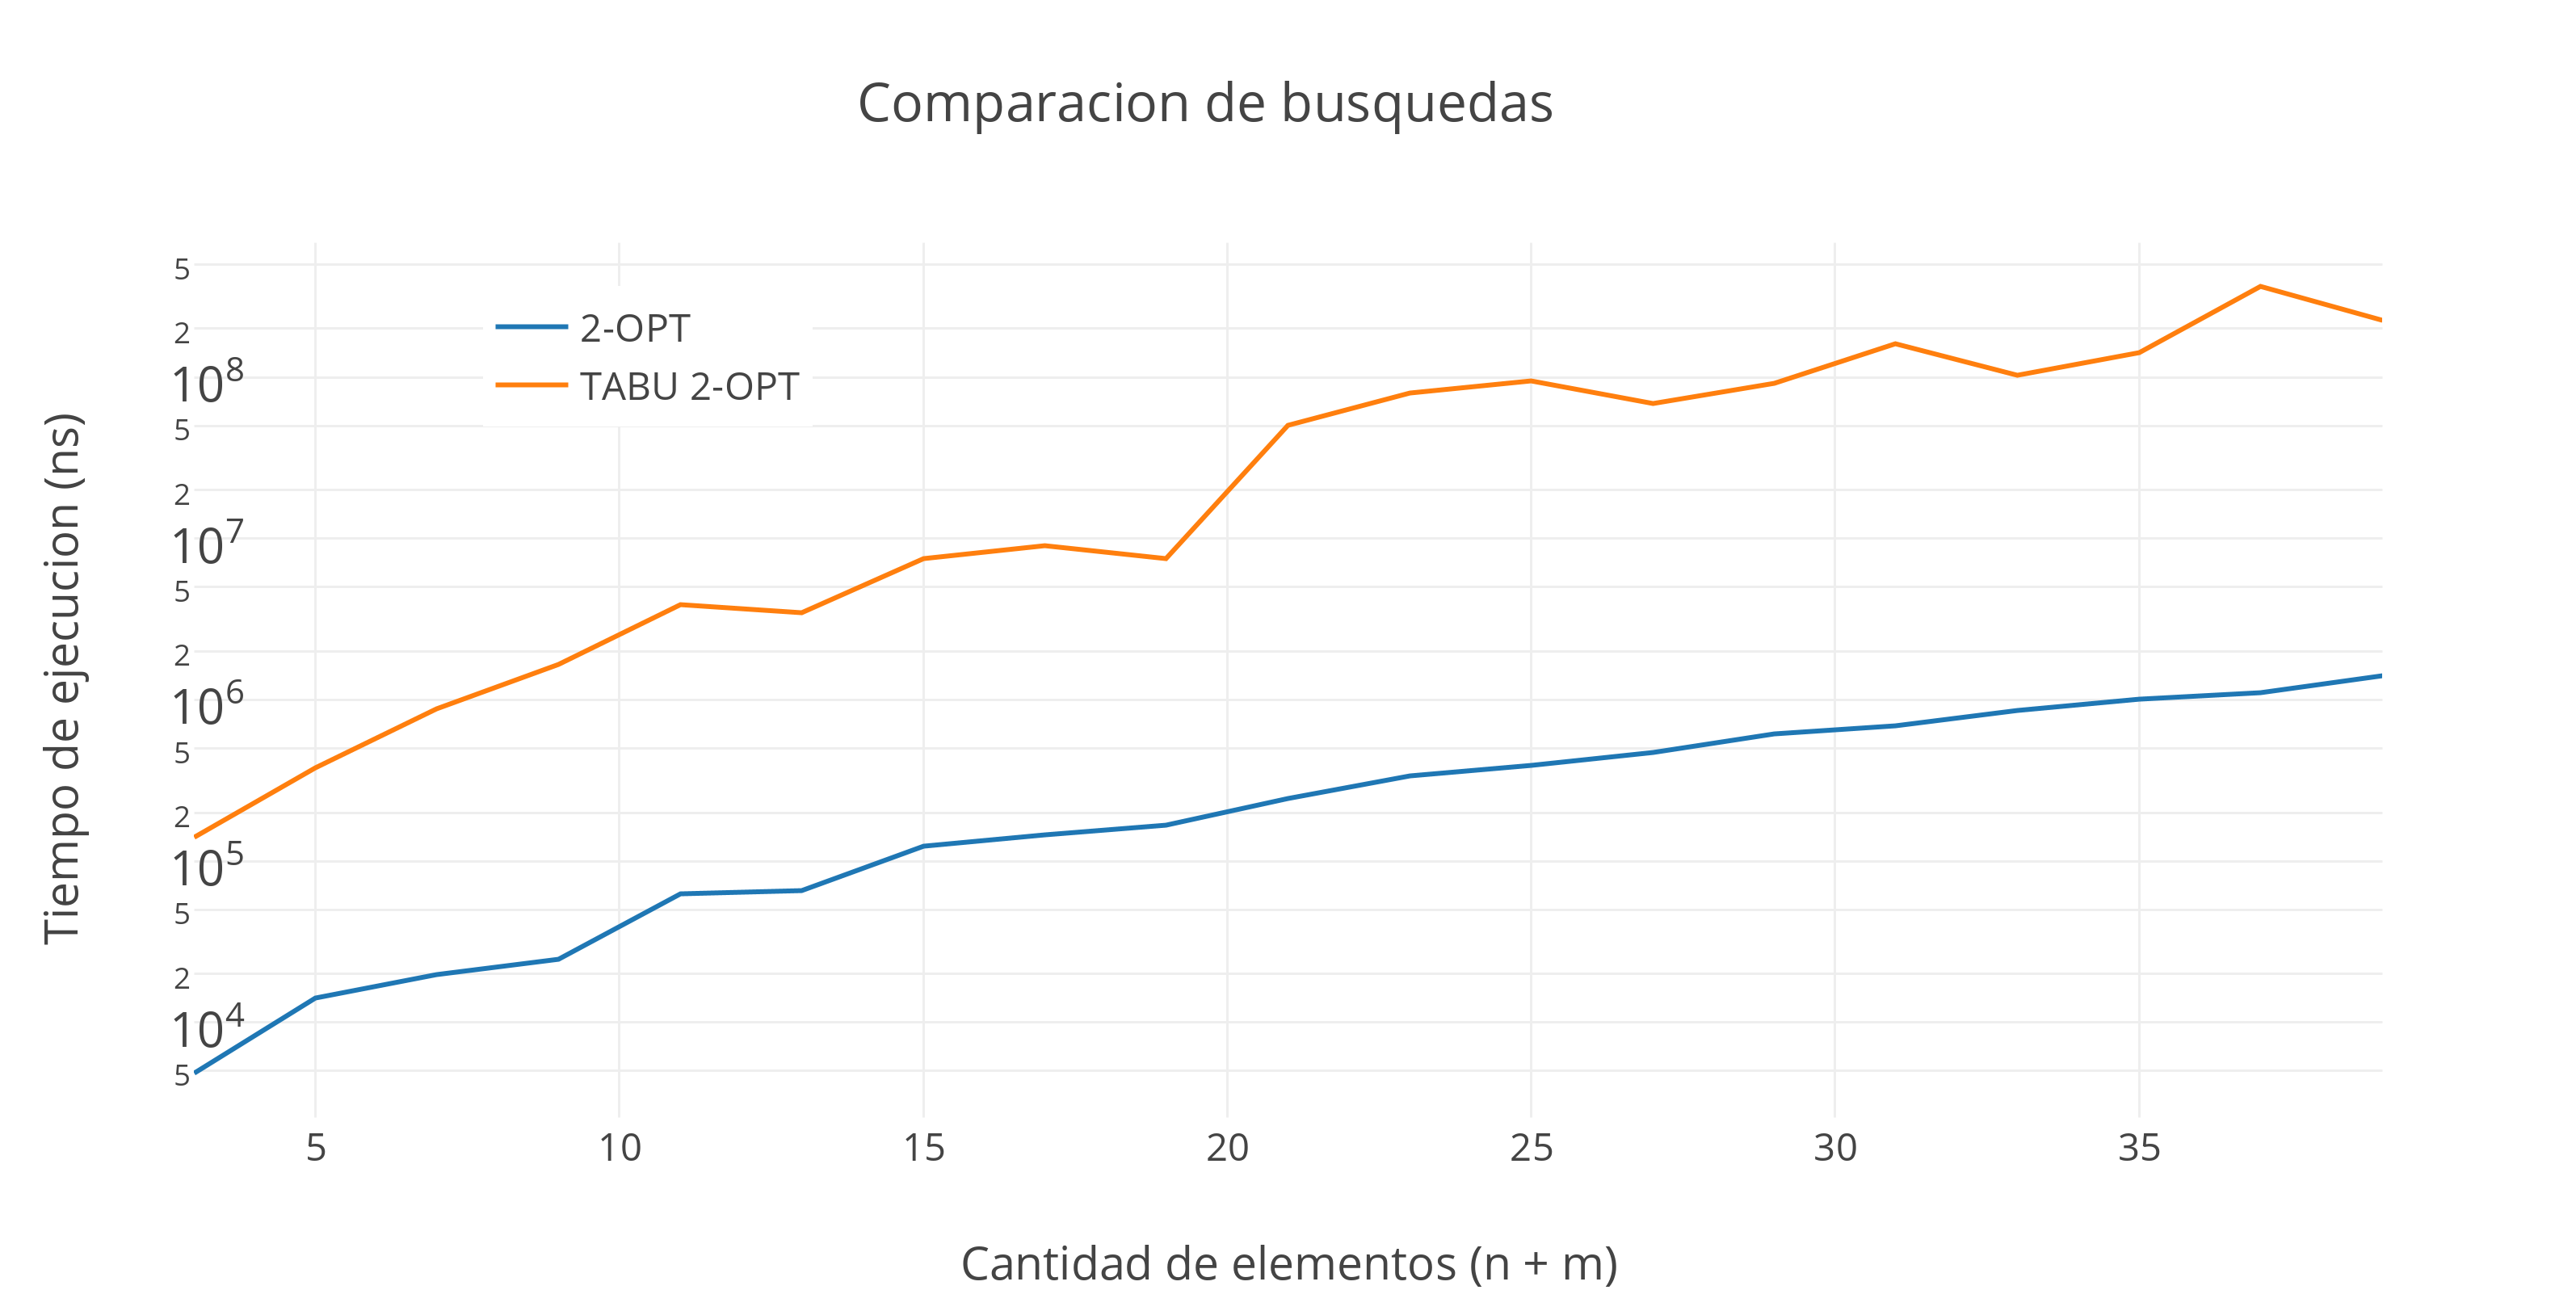
\includegraphics[scale=0.5]{./EJ4/medicion2optgym0.png}\\
 {            \textit{Gráfico \ 4.2 - 2-OPT vs Tabu 2-OPT sobre Familia 4}}
  \end{center}
  \vspace*{0.3cm}
  
 Aplicando 3-OPT:

\vspace*{0.3cm} \vspace*{0.3cm}
  \begin{center}
 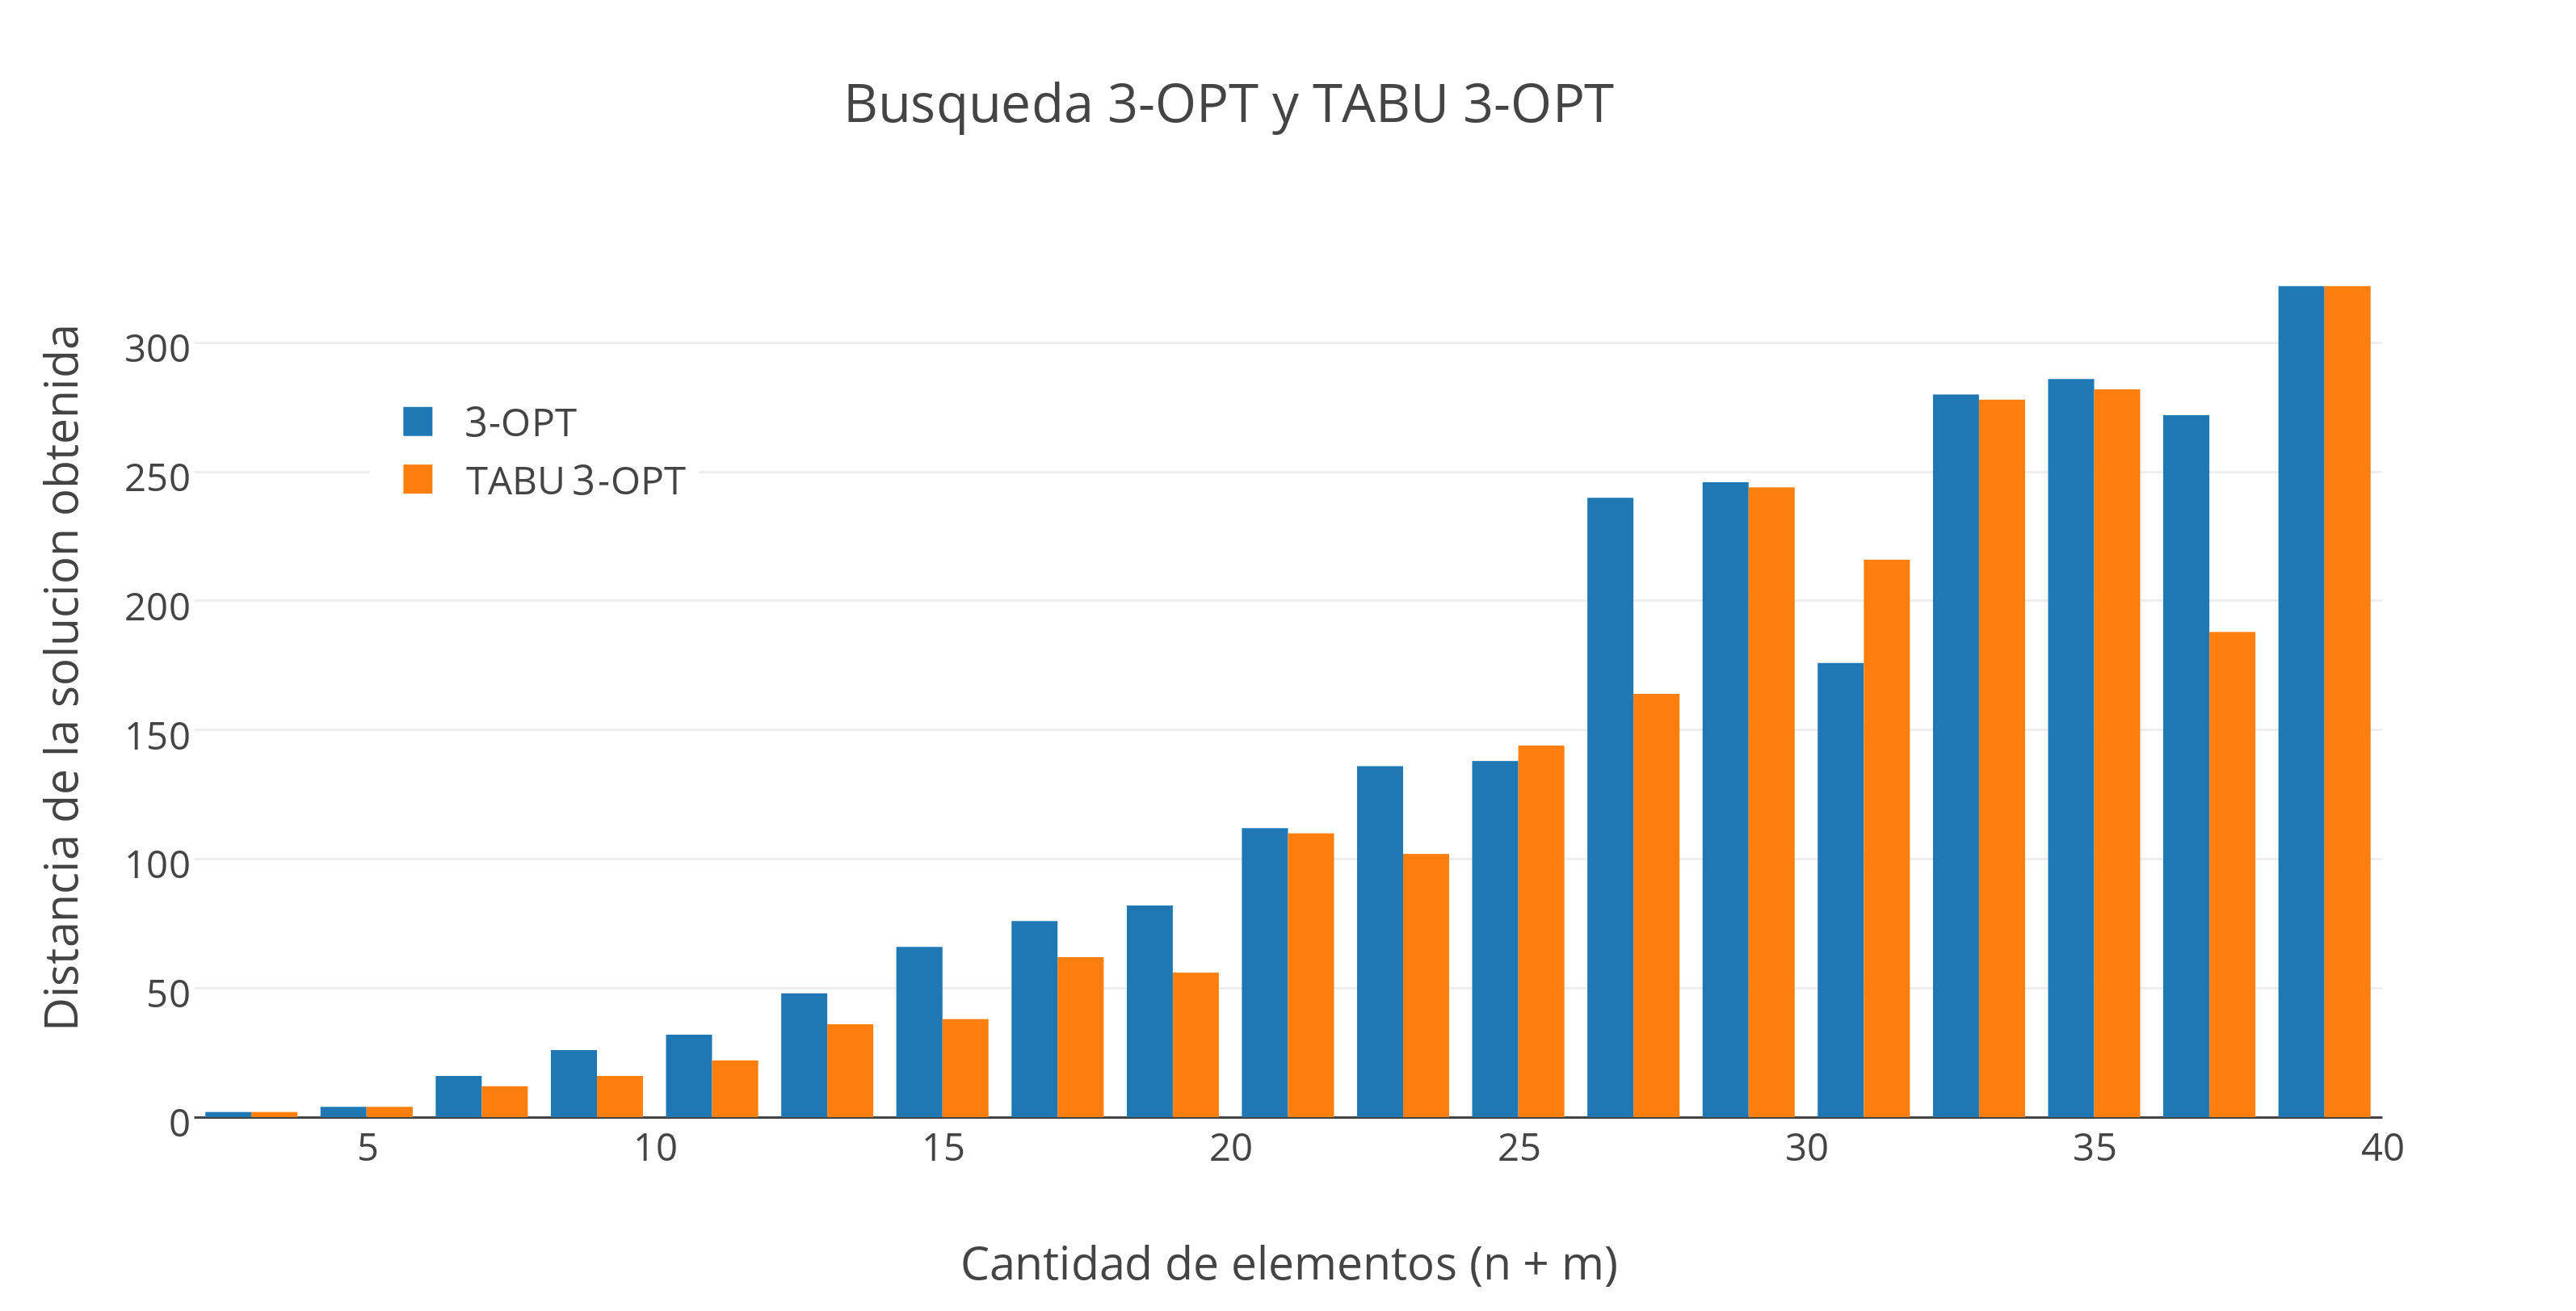
\includegraphics[scale=0.5]{./EJ4/comparativogym03opt.png}\\
 {            \textit{Gráfico \ 4.3 - 3-OPT vs Tabu 3-OPT sobre Familia 4}}
  \end{center}
  \vspace*{0.3cm}

\vspace*{0.3cm} \vspace*{0.3cm}
  \begin{center}
 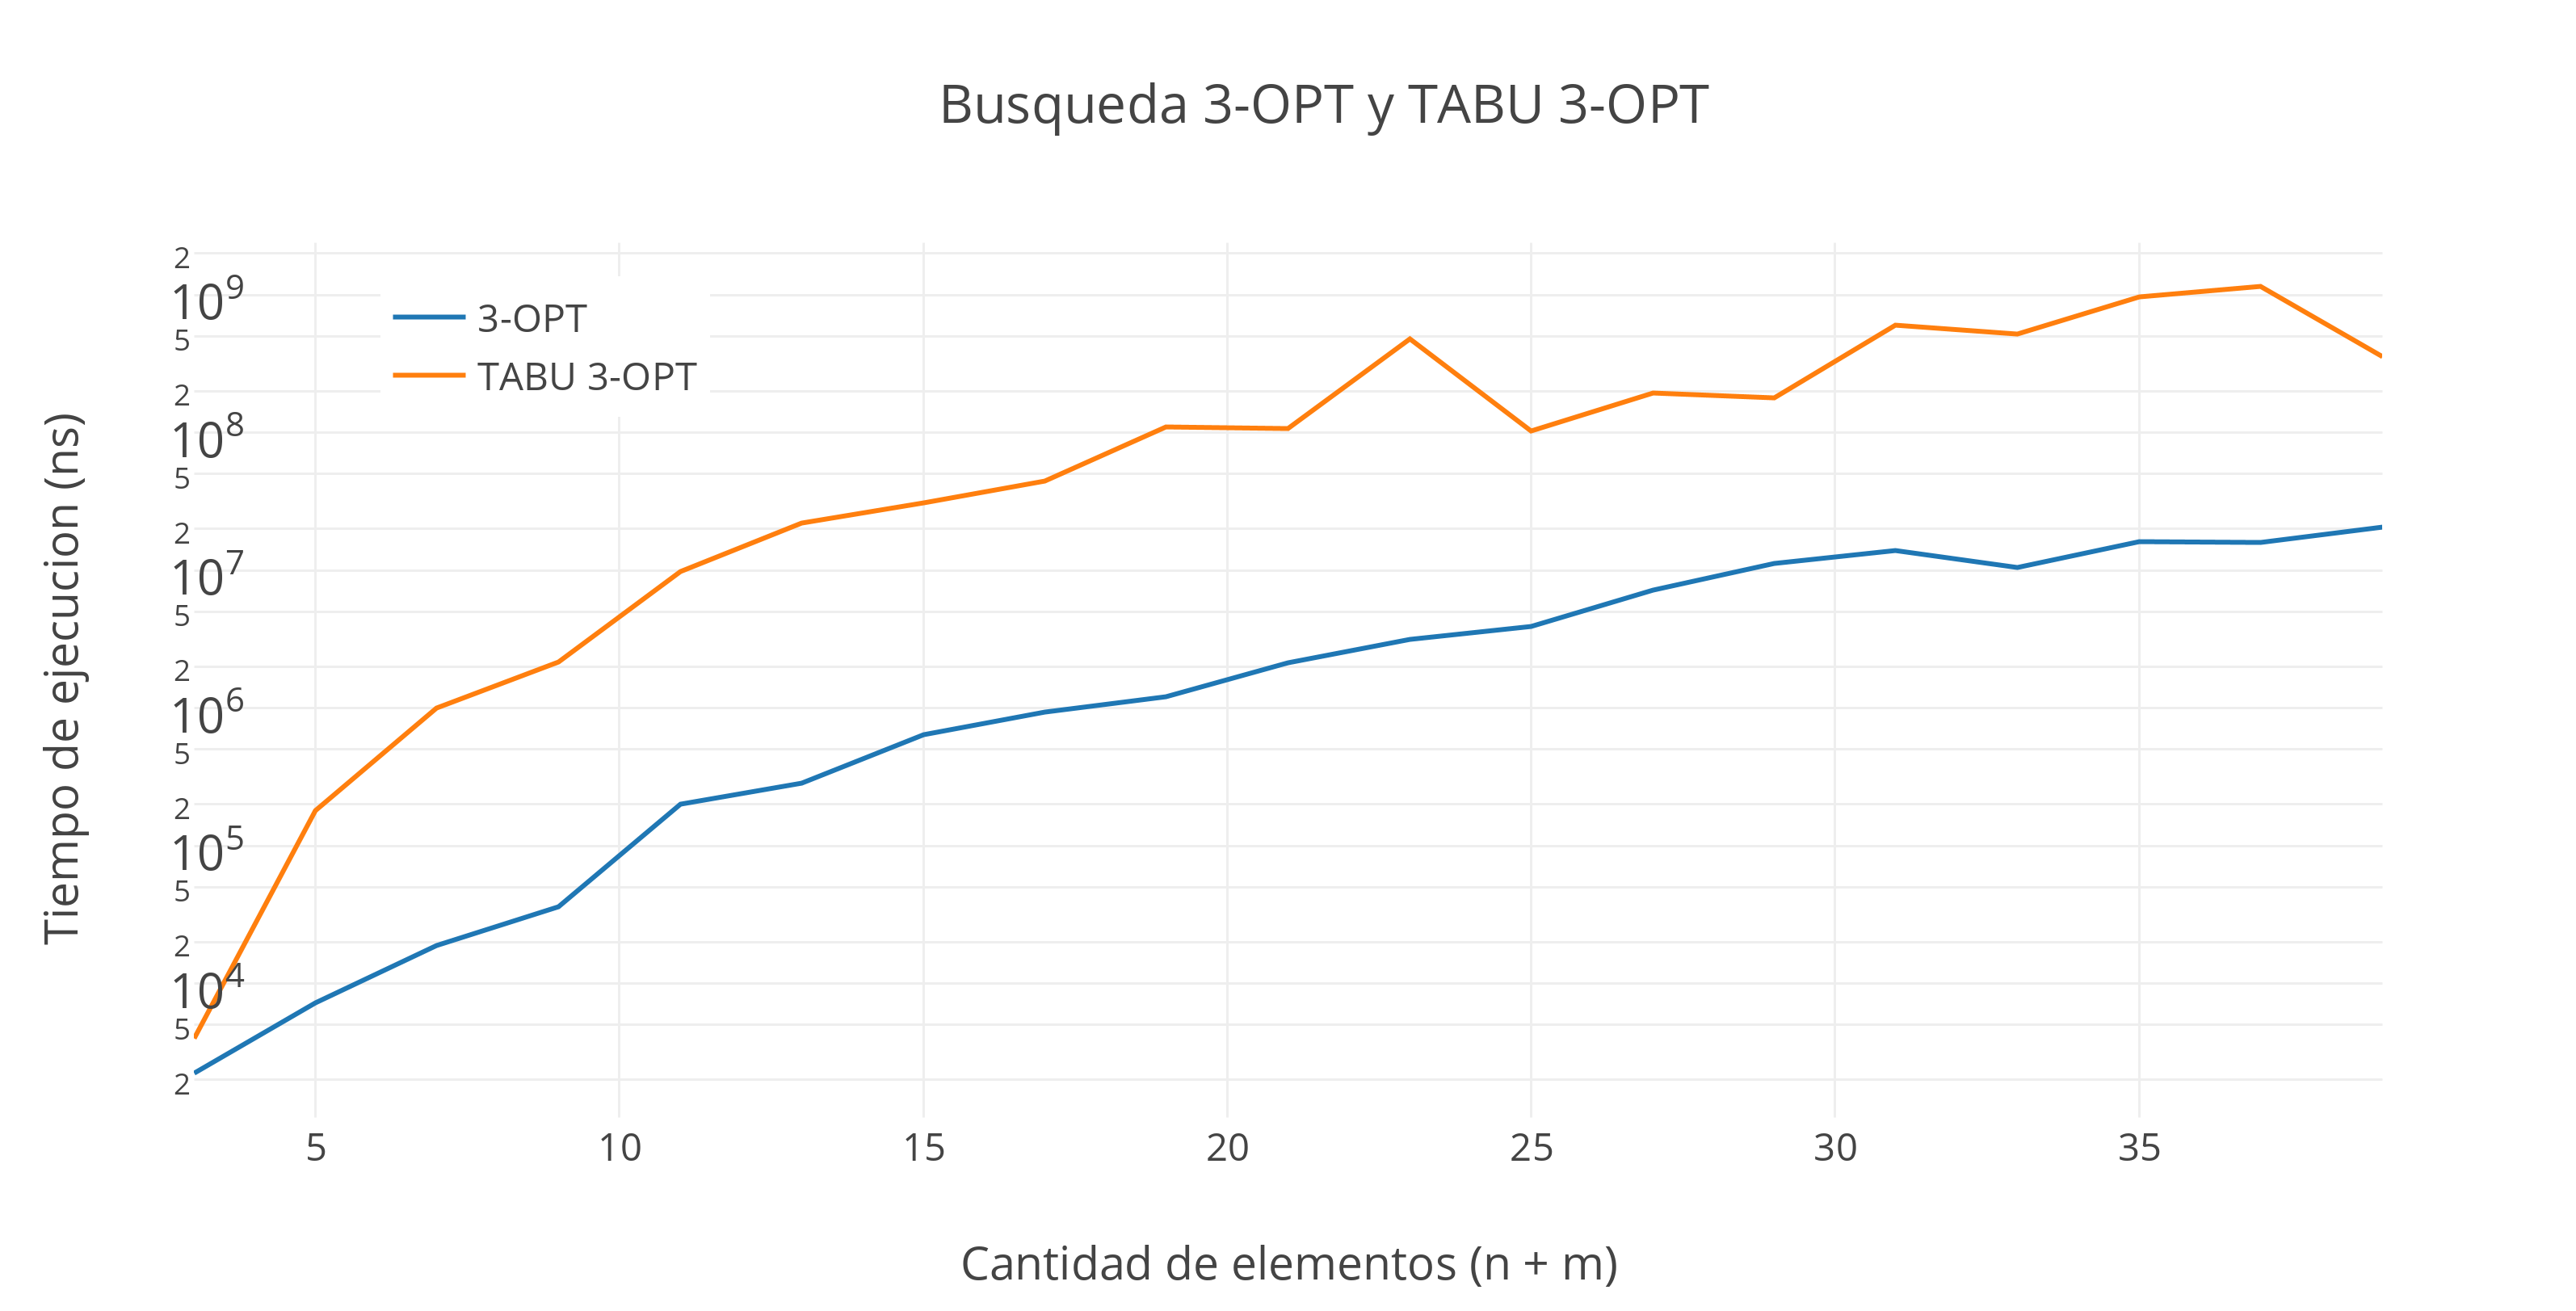
\includegraphics[scale=0.5]{./EJ4/medicion3optgym0.png}\\
 {            \textit{Gráfico \ 4.4 - 3-OPT vs Tabu 3-OPT sobre Familia 4}}
  \end{center}
  \vspace*{0.3cm}
  
Podemos observar que tabú search 2-OPT mejora lo realizado por la heuristica de búsqueda local 2-OPT. Los tiempos insumidos para lograrlo son elevados, pero en relación a la mejora es un resultado aceptable en la práctica. No así tabú search 3-OPT que apenas mejora lo realizado por búsqueda local 3-OPT y requiere tiempos elevados de corrida del algoritmo.\\
  
Para decidir que vecindad es mejor utilizar en tabú search, se comparará conjuntamente el tiempo de ejecución con la calidad de la solución. Para esta última tendremos en cuenta que los algoritmos, de devolver un resultado, serán válidos: esto quiere decir que cuanto menor distancia recorran las soluciones, mejor serán las mismas:

Las soluciones obtenidas fueron las siguientes:

\vspace*{0.3cm} \vspace*{0.3cm}
  \begin{center}
 \includegraphics[scale=0.5]{./EJ4/comparativogym0.png}\\
 {            \textit{Gráfico \ 4.5 - Tabu 2-OPT vs Tabu 3-OPT sobre Familia 4}}
  \end{center}
  \vspace*{0.3cm}

En cuanto a tiempo insumido vemos lo siguiente:

\vspace*{0.3cm} \vspace*{0.3cm}
  \begin{center}
 \includegraphics[scale=0.5]{./EJ4/comparaciongym01.png}\\
 {            \textit{Gráfico \ 4.6 - Tabu 2-OPT vs Tabu 3-OPT sobre Familia 4}}
  \end{center}
  \vspace*{0.3cm}

--> OBTENER CONCLUSIONES

\subsubsection*{Familia 6}

--> PRESENTAR FAMILIA

\vspace*{0.3cm} \vspace*{0.3cm}
  \begin{center}
 \includegraphics[scale=0.3]{./EJ4/fam6goloso.png}\\
 {            \textit{Soluci\'on Golosa}}
  \end{center}
  \vspace*{0.3cm}

\vspace*{0.3cm} \vspace*{0.3cm}
  \begin{center}
 \includegraphics[scale=0.3]{./EJ4/fam62opt.png}\\
 {            \textit{Soluci\'on TABU 2-OPT}}
  \end{center}
  \vspace*{0.3cm}

\vspace*{0.3cm} \vspace*{0.3cm}
  \begin{center}
 \includegraphics[scale=0.3]{./EJ4/fam63opt.png}\\
 {            \textit{Soluci\'on TABU 3-OPT}}
  \end{center}
  \vspace*{0.3cm}

Veamos como se comporta Tabu 2-OPT con respecto a la heuristica de busqueda local 2-OPT:

\vspace*{0.3cm} \vspace*{0.3cm}
  \begin{center}
 \includegraphics[scale=0.5]{./EJ4/comparativosinorden2opt.png}\\
 {            \textit{Gráfico \ 4.7 - 2-OPT vs Tabu 2-OPT sobre Familia 6}}
  \end{center}
  \vspace*{0.3cm}

\vspace*{0.3cm} \vspace*{0.3cm}
  \begin{center}
 \includegraphics[scale=0.5]{./EJ4/medicion2optsinorden.png}\\
 {            \textit{Gráfico \ 4.8 - 2-OPT vs Tabu 2-OPT sobre Familia 6}}
  \end{center}
  \vspace*{0.3cm}

Luego, para 3-OPT:

\vspace*{0.3cm} \vspace*{0.3cm}
  \begin{center}
 \includegraphics[scale=0.5]{./EJ4/comparativogym03opt.png}\\
 {            \textit{Gráfico \ 4.9 - 3-OPT vs Tabu 3-OPT sobre Familia 6}}
  \end{center}
  \vspace*{0.3cm}

\vspace*{0.3cm} \vspace*{0.3cm}
  \begin{center}
 \includegraphics[scale=0.5]{./EJ4/medicion3optsinorden.png}\\
 {            \textit{Gráfico \ 4.10 - 3-OPT vs Tabu 3-OPT sobre Familia 6}}
  \end{center}
  \vspace*{0.3cm}
  
--> OBTENER CONCLUSIONES
  
Comparando las soluciones de cada version de tabú search podemos observar lo siguiente:

\vspace*{0.3cm} \vspace*{0.3cm}
  \begin{center}
 \includegraphics[scale=0.5]{./EJ4/comparativosinorden.png}\\
 {            \textit{Gráfico \ 4.11 - Tabu 2-OPT vs Tabu 3-OPT sobre Familia 6}}
  \end{center}
  \vspace*{0.3cm}

En cuanto a tiempo insumido vemos lo siguiente:

\vspace*{0.3cm} \vspace*{0.3cm}
  \begin{center}
 \includegraphics[scale=0.5]{./EJ4/comparacionsinorden1.png}\\
 {            \textit{Gráfico \ 4.12 - Tabu 2-OPT vs Tabu 3-OPT sobre Familia 6}}
  \end{center}
  \vspace*{0.3cm}
  
--> OBTENER CONCLUSIONES

\subsubsection*{Familia 7}

--> PRESENTAR FAMILIA

\vspace*{0.3cm} \vspace*{0.3cm}
  \begin{center}
 \includegraphics[scale=0.3]{./EJ4/fam7goloso.png}\\
 {            \textit{Soluci\'on Golosa}}
  \end{center}
  \vspace*{0.3cm}

\vspace*{0.3cm} \vspace*{0.3cm}
  \begin{center}
 \includegraphics[scale=0.3]{./EJ4/fam72opt.png}\\
 {            \textit{Soluci\'on TABU 2-OPT}}
  \end{center}
  \vspace*{0.3cm}

\vspace*{0.3cm} \vspace*{0.3cm}
  \begin{center}
 \includegraphics[scale=0.3]{./EJ4/fam73opt.png}\\
 {            \textit{Soluci\'on TABU 3-OPT}}
  \end{center}
  \vspace*{0.3cm}

Veamos como se comporta Tabu 2-OPT con respecto a la heuristica de busqueda local 2-OPT:

\vspace*{0.3cm} \vspace*{0.3cm}
  \begin{center}
 \includegraphics[scale=0.5]{./EJ4/comparativoanillos2opt.png}\\
 {            \textit{Gráfico \ 4.7 - 2-OPT vs Tabu 2-OPT sobre Familia 7}}
  \end{center}
  \vspace*{0.3cm}

\vspace*{0.3cm} \vspace*{0.3cm}
  \begin{center}
 \includegraphics[scale=0.5]{./EJ4/medicionanillos2opt.png}\\
 {            \textit{Gráfico \ 4.8 - 2-OPT vs Tabu 2-OPT sobre Familia 7}}
  \end{center}
  \vspace*{0.3cm}

Luego, para 3-OPT:

\vspace*{0.3cm} \vspace*{0.3cm}
  \begin{center}
 \includegraphics[scale=0.5]{./EJ4/comparativoanillos3opt.png}\\
 {            \textit{Gráfico \ 4.9 - 3-OPT vs Tabu 3-OPT sobre Familia 7}}
  \end{center}
  \vspace*{0.3cm}

\vspace*{0.3cm} \vspace*{0.3cm}
  \begin{center}
 \includegraphics[scale=0.5]{./EJ4/medicionanillos3opt.png}\\
 {            \textit{Gráfico \ 4.10 - 3-OPT vs Tabu 3-OPT sobre Familia 7}}
  \end{center}
  \vspace*{0.3cm}
  
--> OBTENER CONCLUSIONES  
 
Comparando las soluciones de cada version de tabú search podemos observar lo siguiente: 
  
\vspace*{0.3cm} \vspace*{0.3cm}
  \begin{center}
 \includegraphics[scale=0.5]{./EJ4/comparativoanillos1.png}\\
 {            \textit{Gráfico \ 4.11 - Tabu 2-OPT vs Tabu 3-OPT sobre Familia 7}}
  \end{center}
  \vspace*{0.3cm}

\vspace*{0.3cm} \vspace*{0.3cm}
  \begin{center}
 \includegraphics[scale=0.5]{./EJ4/comparativoanillos.png}\\
 {            \textit{Gráfico \ 4.12 - Tabu 2-OPT vs Tabu 3-OPT sobre Familia 7}}
  \end{center}
  \vspace*{0.3cm}

\subsubsection*{Familia 8}

--> PRESENTAR FAMILIA

\vspace*{0.3cm} \vspace*{0.3cm}
  \begin{center}
 \includegraphics[scale=0.3]{./EJ4/fam8goloso.png}\\
 {            \textit{Soluci\'on Golosa}}
  \end{center}
  \vspace*{0.3cm}

\vspace*{0.3cm} \vspace*{0.3cm}
  \begin{center}
 \includegraphics[scale=0.3]{./EJ4/fam82opt.png}\\
 {            \textit{Soluci\'on TABU 2-OPT}}
  \end{center}
  \vspace*{0.3cm}

\vspace*{0.3cm} \vspace*{0.3cm}
  \begin{center}
 \includegraphics[scale=0.3]{./EJ4/fam83opt.png}\\
 {            \textit{Soluci\'on TABU 3-OPT}}
  \end{center}
  \vspace*{0.3cm}

Veamos como se comporta Tabu 2-OPT con respecto a la heuristica de busqueda local 2-OPT:

\vspace*{0.3cm} \vspace*{0.3cm}
  \begin{center}
 \includegraphics[scale=0.5]{./EJ4/comparativorandom2opt.png}\\
 {            \textit{Gráfico \ 4.7 - 2-OPT vs Tabu 2-OPT sobre Familia 8}}
  \end{center}
  \vspace*{0.3cm}

\vspace*{0.3cm} \vspace*{0.3cm}
  \begin{center}
 \includegraphics[scale=0.5]{./EJ4/medicionrandom2opt.png}\\
 {            \textit{Gráfico \ 4.8 - 2-OPT vs Tabu 2-OPT sobre Familia 6}}
  \end{center}
  \vspace*{0.3cm}

Luego, para 3-OPT:

\vspace*{0.3cm} \vspace*{0.3cm}
  \begin{center}
 \includegraphics[scale=0.5]{./EJ4/comparativorandom3opt.png}\\
 {            \textit{Gráfico \ 4.9 - 3-OPT vs Tabu 3-OPT sobre Familia 6}}
  \end{center}
  \vspace*{0.3cm}

\vspace*{0.3cm} \vspace*{0.3cm}
  \begin{center}
 \includegraphics[scale=0.5]{./EJ4/medicionrandom3opt.png}\\
 {            \textit{Gráfico \ 4.10 - 3-OPT vs Tabu 3-OPT sobre Familia 6}}
  \end{center}
  \vspace*{0.3cm}
  
--> OBTENER CONCLUSIONES
  
Comparando las soluciones de cada version de tabú search podemos observar lo siguiente: 

\vspace*{0.3cm} \vspace*{0.3cm}
  \begin{center}
 \includegraphics[scale=0.5]{./EJ4/comparativorandom.png}\\
 {            \textit{Gráfico \ 4.11 - Tabu 2-OPT vs Tabu 3-OPT sobre Familia 6}}
  \end{center}
  \vspace*{0.3cm}

\vspace*{0.3cm} \vspace*{0.3cm}
  \begin{center}
 \includegraphics[scale=0.5]{./EJ4/medicionrandom.png}\\
 {            \textit{Gráfico \ 4.12 - Tabu 2-OPT vs Tabu 3-OPT sobre Familia 6}}
  \end{center}
  \vspace*{0.3cm}
  
--> OBTENER CONCLUSIONES

--> OBTENER CONCLUSIONES GENERALES SOBRE ESTOS TESTS: CUAL VERSION DE TABU CONVIENE MAS? EN QUE CASOS CONVIENE HACER BUSQUEDA LOCAL UNICAMENTE?  
  
--> ANALISIS DEL TRADE OFF: sobre la cantidad de iteraciones y la condicion de corte por producirse limite de no mejoras

\vspace*{0.3cm} \vspace*{0.3cm}
  \begin{center}
 \includegraphics[scale=0.5]{./EJ4/mejora.png}\\
 {            \textit{Gráfico \ 4.12 - Tabu 2-OPT vs Tabu 3-OPT sobre Familia 6}}
  \end{center}
  \vspace*{0.3cm}
  
  \vspace*{0.3cm} \vspace*{0.3cm}
  \begin{center}
 \includegraphics[scale=0.5]{./EJ4/mejora1.png}\\
 {            \textit{Gráfico \ 4.12 - Tabu 2-OPT vs Tabu 3-OPT sobre Familia 6}}
  \end{center}
  \vspace*{0.3cm}
  
  \vspace*{0.3cm} \vspace*{0.3cm}
  \begin{center}
 \includegraphics[scale=0.5]{./EJ4/mejora2.png}\\
 {            \textit{Gráfico \ 4.12 - Tabu 2-OPT vs Tabu 3-OPT sobre Familia 6}}
  \end{center}
  \vspace*{0.3cm}
  
--> OBTENER CONCLUSIONES GENERALES: PORQUE SIRVE? CUANDO CONVIENE ? CUANDO NO ? 
  

%\subsubsection[2.5]{Performance del algorítmo}
%\indent En lo que sigue, mostraremos buenos y malos casos para nuestro algoritmo, y a su vez, daremos el tiempo estimado 
seg\'un la complejidad del algoritmo calculada anteriormente.\\


A continuaci\'on mostraremos un gr\'afico de tiempos comparativo entre distintas familias de casos:\\ 

\vspace*{0.3cm} \vspace*{0.3cm}
  \begin{center}
% \includegraphics[scale=0.4]{./EJ1/comparativo.png}
 {            $Gr$\'a$fico$ \ 1.1 - $Comparativo$}
  \end{center}
  \vspace*{0.3cm}
  
Se puede observar en el gr\'afico, tres funciones las cuales representan el tiempo de ejecuci\'on de las familias de casos:\\
\begin{itemize}
\item Sin soluci\'on o con camino m\'inimo inmediato
\item Rompiendo una cantidad de P-1 paredes
\item M\'ultiples caminos a destino posibles
\end{itemize}


Como se observa en el gr\'afico la funci\'on representativa de la flia n\'umero 1, presenta una mejor performance en relaci\'on a las otras. Esto se debe a que en el primer paso no puede salir por ning\'un camino posible, o su adyacente es el nodo destino por lo tanto chequea solo los nodos adyacentes del origen y finaliza su ejecuci\'on.

Por lo cual, el mejor caso teniendo en cuenta a nivel performance de nuestro algoritmo ser\'a cuando se presente un problema \textbf{Sin soluci\'on o con camino m\'inimo inmediato}

Los grafos que representan lo dicho ser\'ian los siguiente:\\

\vspace*{0.3cm} \vspace*{0.3cm}
  \begin{center}
%\includegraphics[scale=0.65]{./EJ1/ej1grafomejorcaso.jpeg}
{$Ejemplo Grafo$ \ G1.1 - $Mejor$ $Caso$ $Con$ $P=0$ }
  \end{center}
  \vspace*{0.3cm}

\vspace*{0.3cm} \vspace*{0.3cm}
  \begin{center}
%\includegraphics[scale=0.65]{./EJ1/ej1grafomejorcaso2.jpeg}
{$Ejemplo Grafo$ \ G1.1 - $Mejor$ $Caso$ $Con$ $P=0$ }
  \end{center}
  \vspace*{0.3cm}

Para una mayor observaci\'on desarrollamos el siguiente gr\'afico con las instancias:\\

\vspace*{0.3cm} \vspace*{0.3cm}
  \begin{center}
 %\includegraphics[scale=0.65]{./EJ1/mejorcaso.png}
 {$Gr$\'a$fico$ \ 1.1 - $Mejor$ $Caso$}
  \end{center}
  \vspace*{0.3cm}

Como la complejidad que calculamos se basa en la cantidad de nodos posibles que puede haber multiplicado por las paredes contrastaremos nuestras mediciones con los valores de O(F $\times$ C $\times$ P).\\

Luego, dividiendo la funci\'on resultante de nuestro algoritmo sobre el tiempo que demanda realizar O(F $\times$ C $\times$ P) nos da lo siguiente:

\vspace*{0.3cm} \vspace*{0.3cm}
  \begin{center}
 %\includegraphics[scale=0.65]{./EJ1/mejorcaso1.png}
 {$Gr$\'a$fico$ \ 1.2 - $Mejor$ $Caso$ $Sobre$ $Complejidad$ $O(F \times C \times P)$}
  \end{center}
  \vspace*{0.3cm}

 Para obtener dichas instancias nos resulto prudente realizar aproximadamente unas 20 corridas con el mismo input y sacar el promedio de estas 20 corridas para cada instancia para obtener resultados m\'as consisos.\\ 

Se observa en el gr\'afico 1.1 como la funci\'on que representa al tiempo de nuestro algoritmo en el mejor caso es considerablemente mejor que la funci\'on de la cota te\'orica, mientras que al realizar la divisi\'on entre ambas funciones se llega a que la misma nunca supera el valor 0.9 quedando siempre por debajo de 1 mostrando as\'i que para cualquier valor de entrada posible el mejor caso queda siempre en el orden de  O(F $\times$ C $\times$ P).\\

Luego, uno de los peores casos para nuestro algoritmo es en el cual  \textbf{se debe recorrer todos los posibles caminos ya que son todos exactamente iguales}, esto se da as\'i ya que nuestro algoritmo chequea todos los caminos posibles y como todos pueden ser soluci\'on posible avanza por todos y llega al final del laberinto con el mismo valor en todos los posibles caminos\\

\vspace*{0.3cm} \vspace*{0.3cm}
  \begin{center}
%\includegraphics[scale=0.65]{./EJ1/ej1grafopeorcaso.jpeg}
{$Ejemplo Grafo$ \ G1.2 - $Peor$ $Caso$}
  \end{center}
  \vspace*{0.3cm}

Para este grafo realizamos las respectivas mediciones las cuales arrojaron los siguientes resultados:\\


\vspace*{0.3cm} \vspace*{0.3cm}
  \begin{center}
%\includegraphics[scale=0.4]{./EJ1/peorcaso.png}
{$Gr$\'a$fico$ \ 1.3 - $Peor$ $Caso$}
  \end{center}
  \vspace*{0.3cm}

Dividiendo por la complejidad se llego a lo siguiente:\\

\vspace*{0.3cm} \vspace*{0.3cm}
  \begin{center}
%\includegraphics[scale=0.5]{./EJ1/peorcaso1.png}
{$Gr$\'a$fico$ \ 1.4 - $Peor$ $Caso$ $Sobre$ $Complejidad$ $O(F \times C \times P)$}
  \end{center}
  \vspace*{0.3cm}

 Para obtener dichas instancias nos resulto prudente realizar aproximadamente unas 20 corridas con el mismo input y sacar el promedio de estas 20 corridas para cada instancia para obtener resultados m\'as consisos.\\ 

Podemos observar en la figura 1.3 como la funci\'on resultante de nuestro algoritmo en el peor caso se mantiene por debajo de la funci\'on final del tiempo de realizar O(F $\times$ C $\times$ P) operaciones lo cual fue la complejidad precalculada. Y, en el gr\'afico 1.4 es posible observar como la funci\'on obtenida presenta disversos picos los cuales nunca llegan a superar 1, y cuando el tamaño de entrada aumenta la funci\'on queda asintotizada por 0.95.\\

Por \'ultimo mostraremos un gr\'afico comparativo con el mejor, el peor y el caso promedio contra la complejidad precalculada .\\

  
  \vspace*{0.3cm} \vspace*{0.3cm}
  \begin{center}
%\includegraphics[scale=0.4]{./EJ1/comparativo1.png}
{$Gr$\'a$fico$ \ 1.5 - $Comparativo$}
  \end{center}
  \vspace*{0.3cm}
  
 Es visible en este gr\'afico comparativo como las funciones relacionadas a nuestro algoritmo estan acotadas por la funci\'on de la complejidad te\'orica.

Mostraremos a continuaci\'on un caso en el cual se dejaron fijas las variables F y C, ambas en 50 y se trabajo con P movil para ver como se comporta nuestro algoritmo en esta situaci\'on.

\vspace*{0.3cm} \vspace*{0.3cm}
  \begin{center}
%\includegraphics[scale=0.65]{./EJ1/pMovil.png}
{$Gr$\'a$fico$ \ 1.6 - $P$ $movil$ $y$ $F,C$ $Fijos$}
  \end{center}
  \vspace*{0.3cm}

Se puede observar en el gr\'afico 1.6 como al trabajar con este caso en el cual a medida que P aumenta es necesario romper P paredes para llegar a destino, la funci\'on resultante se comporta de la misma manera que O(P), chequeando de esta forma que trabajando con una cantidad fija de nodos nuestro algoritmo realiza O(P) operaciones por cada elemento del grafo.\\

Luego de lo mostrado, se pudo observar que, tanto en el mejor como en el peor caso nuestro algoritmo se encuentra en el orden de la complejidad calculada.

\newpage
\section{Ejercicio 5} 
\subsection{Descripción de nuevas instancias y experimentación}
Para este punto se desarrollaron nuevas instancias random distintas a las anteriores. Se realizaron nuevas experimentaciones para corroborar la performance y calidad de soluci\'on de cada heuristica

Un ejemplo de dichas instancias es el siguiente:

\vspace*{0.3cm} \vspace*{0.3cm}
  \begin{center}
\includegraphics[scale=0.5]{./EJ5/caminoEjGoloso.png}
\\{\textit{Resultado goloso}}
  \end{center}
  \vspace*{0.3cm}
----> PONER UN GRAFICO DE BL Y OTRO DE TABU

\subsubsection{Comparaciones de performance entre heuristicas}

Para corroborar la performance obtenida para este grupo de instancias se tomaron los tiempos que tarda cada algoritmo en obtener soluci\'on.

Dicho conjunto esta formado por un total de 50 instancias que van desde 2 elementos hasta 50 en total.

-----> GRAFICO DE MEDICIONES 






\subsubsection*{Comparacion contra backtraking}
INSERTAR LA HEURISTICA MAS LENTA VS BACKTRACKING
\subsubsection{Comparacion de calidad de solución}
INSERTAR GRAFICOS DE BOXPLOTS ENTRE LOS ERRORES DE CADA HEURISTICA:
	ERROR VS TAMAÑO DE ENTRADA POR CADA HEURISTICA (cada columna que forme un boxplot en el grafico comparativo)
	


\newpage
\section{Aclaraciones} 
\subsection{Aclaraciones para correr las implementaciones}
\subsection{Dificultades afrontadas}

A lo largo del desarrollo del trabajo nos encontramos con ciertos obstáculos que tuvimos que ir sorteando:
El primero de ellos fue el tiempo necesario para correr los tests: Al manejar un algoritmo de tiempo exponencial, como es el backtraking, tuvimos que limitarnos a un pequeño grupo de instancias para obtener las mediciones exactas para las comparaciones con otros algoritmos. La utilización de la optimización en la compilación de nivel 3 (-O3) ayudo en grán medida a correr los casos más grandes y poder agrandar un poco más la muestra.\\
A la hora de tomar las mediciones de los experimentos, nos vimos con el problema de la cantidad de instancias de un mismo tamaño a tomar: siendo que no podemos tomar la misma cantidad por cada tamaño debido a que acarrea un desbalance de exactitud (las instancias más chicas tendrían más datos muestrales que las grandes), tuvimos que adaptar la muestra al n(n+m) evaluado. Esto nos ocasionó un incremento substancial en la cantidad de instancias totales a evaluar, incrementando asi el tiempo de experimetación.\\

\subsection{Aclaraciones para correr las implementaciones}

Cada ejercicio fue implementado con su propio Makefile para un correcto funcionamiento a la hora de utilizar el mismo.\\
El ejecutable para el ejercicio 1 sera ej1 el cual recibir\'a como se solicito entrada por stdin y emitir\'a su respectiva salida por stdout.\\
Tanto el ejercicio 2 como el 3 y 4, compilar\'an de la misma forma y podr\'an ser ejecutados con ej2, ej3 y ej4 respectivamente.\\
A su vez, para poder chequear las mediciones de tiempo y nuestros casos de testeo se creo una carpeta nueva por cada ejercicio. Dentro de cada una se cuenta con el respectivo makefile que compila todos los test pudiendo as\'i probar cada uno por separado.

\end{document}
